%%%%%% Run at command line, run
%%%%%% xelatex grad-sample.tex 
%%%%%% for a few times to generate the output pdf file
\documentclass[12pt,oneside,openright,a4paper]{cpe-thai-project}


\usepackage{polyglossia}
\usepackage{enumitem,lipsum}
\usepackage{graphicx}
\usepackage{placeins}
\usepackage{tabularx}
\usepackage{multirow}
\usepackage{colortbl}
\usepackage{graphicx}
\usepackage[table,xcdraw]{xcolor}

\graphicspath{ {./images/} }
\setdefaultlanguage{thai}
\setotherlanguage{english}
\newfontfamily\thaifont[Script=Thai,Scale=1.23]{TH Sarabun New}
\defaultfontfeatures{Mapping=tex-text,Scale=1.23,LetterSpace=0.0}
\setmainfont[Scale=1.23,LetterSpace=0,WordSpace=1.0,FakeStretch=1.0,Mapping=tex-text]{TH Sarabun New}
\XeTeXlinebreaklocale "th"	
\XeTeXlinebreakskip = 0pt plus 0pt
\emergencystretch=10pt

%%%%%%%%%%%%%%%%%%%%%%%%%%%%%%%%%%%%%%%%%%%%%%%%%%%%%%%%%%%%%%%%%%%
% Customize below to suit your needs 
% The ones that are optional can be left blank. 
%%%%%%%%%%%%%%%%%%%%%%%%%%%%%%%%%%%%%%%%%%%%%%%%%%%%%%%%%%%%%%%%%%%
% First line of title
\def\disstitleone{Will Chain }   
% Second line of title
\def\disstitletwo{Will On Blockchain}   
% Your first name and lastname
\def\dissauthor{MR. THITIPONG BOONTHANAKORN}   % 1st member
%%% Put other group member names here ..
\def\dissauthortwo{MR. NARONGYOT SOONTHARARAK}   % 2nd member (optional)
\def\dissauthorthree{MR. SUBTAWEE NGANRUNGRUANG}   % 3rd member (optional)


% The degree that you're persuing..
\def\dissdegree{Bachelor of Engineering} % Name of the degree
\def\dissdegreeabrev{B.Eng} % Abbreviation of the degree
\def\dissyear{2022}                   % Year of submission
\def\thaidissyear{2565}               % Year of submission (B.E.)

%%%%%%%%%%%%%%%%%%%%%%%%%%%%%%%%%%%%%%%%%%%%
% Your project and independent study committee..
%%%%%%%%%%%%%%%%%%%%%%%%%%%%%%%%%%%%%%%%%%%%
\def\dissadvisor{Asst.Prof. Marong Phadoongsidhi, Ph.D.}  % Advisor
%%% Leave it empty if you have no Co-advisor
\def\disscoadvisor{}  % Co-advisor
\def\disscommitteetwo{Mrs. Piyanit Wepulanon , Ph.D.}  % 3rd committee member (optional)
\def\disscommitteethree{Asst.Prof. Thumrongrat Amornraksa , Ph.D.}
\def\disscommitteefour{Asst.Prof. Surapont Toomnark}    % 5th committee member (optional) 

\def\worktype{Project} %%  Project or Independent study
\def\disscredit{3}   %% 3 credits or 6 credits


\def\fieldofstudy{Computer Engineering} 
\def\department{Computer Engineering} 
\def\faculty{Engineering}

\def\thaifieldofstudy{วิศวกรรมคอมพิวเตอร์} 
\def\thaidepartment{วิศวกรรมคอมพิวเตอร์} 
\def\thaifaculty{วิศวกรรมศาสตร์}
 
\def\appendixnames{Appendix} %%% Appendices or Appendix

\def\thaiworktype{ปริญญานิพนธ์} %  Project or research project % 
\def\thaidisstitleone{Will Chain}
\def\thaidisstitletwo{Will on Blockchain}
\def\thaidissauthor{นายฐิติพงศ์ บุณธนากร}
\def\thaidissauthortwo{นายณรงค์ยศ สุนทรารักษ์} %Optional
\def\thaidissauthorthree{นายทรัพย์ทวี งานรุ่งเรือง} %Optional

\def\thaidissadvisor{ผศ.ดร.มารอง ผดุงสิทธิ์}
%% Leave this empty if you have no co-advisor
\def\thaidisscoadvisor{รศ.ดร.ที่ปรึกษา วิทยานิพนธ์ร่วม} %Optional
\def\thaidissdegree{วิศวกรรมศาสตรบัณฑิต}

% Change the line spacing here...
\linespread{1.15}

%%%%%%%%%%%%%%%%%%%%%%%%%%%%%%%%%%%%%%%%%%%%%%%%%%%%%%%%%%%%%%%%
% End of personal customization.  Do not modify from this part 
% to \begin{document} unless you know what you are doing...
%%%%%%%%%%%%%%%%%%%%%%%%%%%%%%%%%%%%%%%%%%%%%%%%%%%%%%%%%%%%%%%%


%%%%%%%%%%%% Dissertation style %%%%%%%%%%%
%\linespread{1.6} % Double-spaced  
%%\oddsidemargin    0.5in
%%\evensidemargin   0.5in
%%%%%%%%%%%%%%%%%%%%%%%%%%%%%%%%%%%%%%%%%%%
%\renewcommand{\subfigtopskip}{10pt}
%\renewcommand{\subfigbottomskip}{-5pt} 
%\renewcommand{\subfigcapskip}{-6pt} %vertical space between caption
%                                    %and figure.
%\renewcommand{\subfigcapmargin}{0pt}

\renewcommand{\topfraction}{0.85}
\renewcommand{\textfraction}{0.1}

\newtheorem{theorem}{Theorem}
\newtheorem{lemma}{Lemma}
\newtheorem{corollary}{Corollary}

\def\QED{\mbox{\rule[0pt]{1.5ex}{1.5ex}}}
\def\proof{\noindent\hspace{2em}{\itshape Proof: }}
\def\endproof{\hspace*{\fill}~\QED\par\endtrivlist\unskip}
%\newenvironment{proof}{{\sc Proof:}}{~\hfill \blacksquare}
%% The hyperref package redefines the \appendix. This one 
%% is from the dissertation.cls
%\def\appendix#1{\iffirstappendix \appendixcover \firstappendixfalse \fi \chapter{#1}}
%\renewcommand{\arraystretch}{0.8}
%%%%%%%%%%%%%%%%%%%%%%%%%%%%%%%%%%%%%%%%%%%%%%%%%%%%%%%%%%%%%%%%
%%%%%%%%%%%%%%%%%%%%%%%%%%%%%%%%%%%%%%%%%%%%%%%%%%%%%%%%%%%%%%%%

\usepackage{ragged2e}
\begin{document}

\pdfstringdefDisableCommands{%
\let\MakeUppercase\relax
}

\begin{center}
  
\includegraphics[width=2.8cm]{logo02.jpg}
\end{center}
\vspace*{-1cm}

\maketitlepage
\makesignaturepage 

%%%%%%%%%%%%%%%%%%%%%%%%%%%%%%%%%%%%%%%%%%%%%%%%%%%%%%%%%%%%%%
%%%%%%%%%%%%%%%%%%%%%% English abstract %%%%%%%%%%%%%%%%%%%%%%%
%%%%%%%%%%%%%%%%%%%%%%%%%%%%%%%%%%%%%%%%%%%%%%%%%%%%%%%%%%%%%%
\abstract

Will Chain is a platform developed with the aim of studying how Blockchain networks work and managing wills in real-world assets. and digital assets. Will Chain will include features for managing and keeping current wills. that can meet both real-life assets and digital assets There will be a feature that will support the addition of a will, namely a feature for delivering assets to beneficiary. If the conditions are the same as in the will Makes wills more secure It is also convenient to make wills. and will have even greater coverage.

\begin{flushleft}
\begin{tabular*}{\textwidth}{@{}lp{0.8\textwidth}}
\textbf{Keywords}: & Asset / Blockchain / Cryptocurrency / Digital Asset / Non-Fungible Token (NFT) /  Smart Contract / Will 
\end{tabular*}
\end{flushleft}
\endabstract

%%%%%%%%%%%%%%%%%%%%%%%%%%%%%%%%%%%%%%%%%%%%%%%%%%%%%%%%%%%%%%
%%%%%%%%%% Thai abstract here %%%%%%%%%%%%%%%%%%%%%%%%%%%%%%%%%
%%%%%%%%%%%%%%%%%%%%%%%%%%%%%%%%%%%%%%%%%%%%%%%%%%%%%%%%%%%%%%
% {\newfontfamily\thaifont{TH Sarabun New:script=thai}[Scale=1.3]
% \XeTeXlinebreaklocale "th_TH"	
% \thaifont
\newcommand\tab[1][1cm]{\hspace*{#1}}
\thaiabstract

\tab Will Chain เป็นแพลตฟอร์มที่ถูกพัฒนาขึ้นมาโดยมีวัตถุประสงค์เพื่อศึกษาการทำงานของเครือข่าย Blockchain  และจัดการเกี่ยวกับพินัยกรรมในด้านของสินทรัพย์ในโลกความเป็นจริง และสินทรัพย์ดิจิทัล โดยที่ Will Chain นั้นจะมีฟีเจอร์ในการจัดการและเก็บรักษาพินัยกรรมที่มีอยู่ในปัจจุบัน ที่จะสามารถตอบโจทย์ได้ทั้งสินทรัพย์ในชีวิตจริงและสินทรัพย์ดิจิทัล โดยจะมีฟีเจอร์ที่จะรองรับการทำพินัยกรรมเพิ่มเติมคือฟีเจอร์สำหรับการส่งมอบสินทรัพย์ให้กับทายาท ถ้ามีเงื่อนไขตรงกับในพินัยกรรม ทำให้การทำพินัยกรรมนั้นมีความปลอดภัยมากขึ้น อีกทั้งสะดวกในการทำพินัยกรรม และจะมีความครอบคลุมที่มากยิ่งขึ้น
\begin{flushleft}
\begin{tabular*}{\textwidth}{@{}lp{0.8\textwidth}}
 & \\

\textbf{คำสำคัญ}: & Asset / Blockchain / Cryptocurrency / Digital Asset / Non-Fungible Token (NFT) /  Smart Contract / Will 
\end{tabular*}
\end{flushleft}
\endabstract

%}

%%%%%%%%%%%%%%%%%%%%%%%%%%%%%%%%%%%%%%%%%%%%%%%%%%%%%%%%%%%%
%%%%%%%%%%%%%%%%%%%%%%% Acknowledgments %%%%%%%%%%%%%%%%%%%%
%%%%%%%%%%%%%%%%%%%%%%%%%%%%%%%%%%%%%%%%%%%%%%%%%%%%%%%%%%%%
\preface
\tab การทําโครงงานครั้งนี้สําเร็จลงได้ด้วยความช่วยเหลือของ ผู้ช่วยศาสตราจารย์ ดร. มารอง ผดุงสิทธิ์ ที่ปรึกษาโครงงาน ซึ่งได้ให้ความกรุณา สละเวลาให้คําปรึกษา คําแนะนํา ข้อเสนอแนะอันมีประโยชน์อย่างมาก และความช่วยเหลือตลอดการทําโครงงานนี้จนสําเร็จลุล่วงได้ด้วยดี ผู้จัดทําโครงงานจึงขอกราบขอบพระคุณเป็นอย่างสูง

\tab ขอขอบพระคุณวราณัฐ สุทธิการณ ซึ่งได้ให้ความกรุณาสละเวลาให้คําแนะนําการออกแบบ Smart Contract และความช่วยเหลือตลอดการทำโครงการนี้

\tab ขอขอบพระคุณ ผ.ศ.สุรพนธ์ ตุ้มนาค , ดร.ปิยนิตย์ เวปุลานนท์ และ รศ.ดร.ธํารงรัตน์ อมรรักษา ที่ได้สละเวลา
ร่วมเป็นคณะกรรมการตรวจสอบโครงงานในครั้งนี้ 

\tab ท้ายที่สุดนี้ โครงงานนี้อาจจะไม่สําเร็จเลยหากไม่มีเพื่อนในภาควิชาวิศวกรรมคอมพิวเตอร์ มหาวิทยาลัยเทคโนโลยีพระจอมเกล้าธนบุรีที่ให้ 
ความช่วยเหลือ การสนับสนุน รวมทั้งคอยเป็นกําลังใจสําคัญเสมอมา 

\tab ทีมผู้จัดทำหวังว่าโครงงานนี้จะก่อให้เกิดประโยชน์ต่อการทำพินัยกรรมในปัจจุบัน และสามารถครอบคลุมไปถึงพินัยกรรมของสินทรัพย์ดิจิทัลที่ยังไม่มีเทคโนโลยีรองรับในตอนนี้ และเกิดการเปลี่ยนแปลงที่ดีขึ้นในอนาคต

%%%%%%%%%%%%%%%%%%%%%%%%%%%%%%%%%%%%%%%%%%%%%%%%%%%%%%%%%%%%%
%%%%%%%%%%%%%%%% ToC, List of figures/tables %%%%%%%%%%%%%%%%
%%%%%%%%%%%%%%%%%%%%%%%%%%%%%%%%%%%%%%%%%%%%%%%%%%%%%%%%%%%%%
% The three commands below automatically generate the table 
% of content, list of tables and list of figures
\tableofcontents                    
\listoftables
\listoffigures                      

%%%%%%%%%%%%%%%%%%%%%%%%%%%%%%%%%%%%%%%%%%%%%%%%%%%%%%%%%%%%%%
%%%%%%%%%%%%%%%%%%%%% List of symbols page %%%%%%%%%%%%%%%%%%%
%%%%%%%%%%%%%%%%%%%%%%%%%%%%%%%%%%%%%%%%%%%%%%%%%%%%%%%%%%%%%%
% You have to add this manually..
%\listofsymbols
%
%%%%%%%%%%%%%%%%%%%%%%%%%%%%%%%%%%%%%%%%%%%%%%%%%%%%%%%%%%%%%%
%%%%%%%%%%%%%%%%%%%%% List of vocabs & terms %%%%%%%%%%%%%%%%%
%%%%%%%%%%%%%%%%%%%%%%%%%%%%%%%%%%%%%%%%%%%%%%%%%%%%%%%%%%%%%%
% You also have to add this manually..
\listofvocab
\begin{flushleft}
\begin{tabular}{@{}p{1in}@{=\extracolsep{0.5in}}l}
Asset & ทรัพย์สินที่เรามีอยู่ทั้งหมด  เงินที่อยู่ในบัญชีทั้งหมดอยู่ในกระเป๋าทั้งหมดรวมทั้งหนี้สินที่เรามีอยู่ทั้งหมด \\
Blockchain & ระบบโครงข่ายในการเก็บบัญชีธุรกรรมออนไลน์ \\
Cryptocurrency & สกุลเงินเข้ารหัส เป็นสินทรัพย์ดิจิทัล \\
Digital Asset & สิ่งที่มีมูลค่าและเราสามารถเป็นเจ้าของได้ แต่ไม่สามารถแตะต้องได้ทางกายภาพ\\
Non-Fungible Token(NFT) & สิ่งของที่มีความแตกต่างเฉพาะตัวไม่สามารถทดแทนกันได้หรือซื้อเป็นหน่วยย่อยได้\\
Smart Contract & กระบวนการทางดิจิทัล ที่กำหนดขั้นตอนการทำธุรกรรมโดยอัตโนมัติไว้ล่วงหน้า โดยไม่ต้องอาศัยตัวกลาง\\
Will  & พินัยกรรมที่เก็บคำสั่งเสียสุดท้ายในการทำกิจการต่าง ๆ \\
\end{tabular}
\end{flushleft}

%\setlength{\parskip}{1.2mm}

%%%%%%%%%%%%%%%%%%%%%%%%%%%%%%%%%%%%%%%%%%%%%%%%%%%%%%%%%%%%%%%
%%%%%%%%%%%%%%%%%%%%%%%% Main body %%%%%%%%%%%%%%%%%%%%%%%%%%%%
%%%%%%%%%%%%%%%%%%%%%%%%%%%%%%%%%%%%%%%%%%%%%%%%%%%%%%%%%%%%%%%


\chapter{บทนำ}

\section{ที่มาและความสำคัญ}

\tab ในปัจจุบันนั้นเทคโนโลยีเข้ามามีบทบาทในการใช้ชีวิตของผู้คนเป็นอย่างมาก ไม่ว่าจะเป็นในด้านของ การเงิน สินทรัพย์ เป็นต้น แต่ว่าจะมีในด้านของพินัยกรรมที่นับว่าเป็นเอกสารที่ไม่มีการใช้เทคโนโลยีเข้ามาช่วยเหลือในปัจจุบัน โดยยังที่จะต้องทำการเก็บรักษาไว้ที่ตัวเองหรือไม่ก็เก็บไว้ที่ทนายของตนเองทำให้บางครั้งพินัยกรรมนั้น ๆ อาจเกิดการเสียหายหรือสูญหายได้ หรือแม้กระทั่งอาจเกิดโอกาสเปลี่ยนแปลงจากบุคคลที่สามได้ ทำให้การทำพินัยกรรมในแต่ละครั้งมีความยุ่งยากและไม่ปลอดภัยสำหรับผู้ที่จะทำพินัยกรรม รวมถึงพินัยกรรมในส่วนนี้ยังครอบคลุมในด้านของการสืบทอดสินทรัพย์ดิจิทัล อย่างเช่น Cryptocurrency ได้ เนื่องจากยังไม่มีเทคโนโลยีที่รองรับในปัจจุบัน

\tab จึงเกิดแนวคิดที่จะสร้าง แพลตฟอร์มสำหรับจัดการพินัยกรรมทั้งสินทรัพย์ในโลกความเป็นจริง และสินทรัพย์ดิจิทัลผ่านระบบ Blockchain\ ที่สามารถนำพินัยกรรมที่มีอยู่ในปัจจุบันนั้นเอาขึ้นระบบ Blockchain เพื่อเก็บรักษาพินัยกรรมนั้น และสามารถทำการสืบทอดสินทรัพย์ไปยังผู้รับพินัยกรรมได้ รวมไปถึงสินทรัพย์ดิจิทัลอีกด้วย โดยคำนึงถึงความปลอดภัยและความสะดวกสบายของผู้ใช้งาน


\section{วัตถุประสงค์}

\begin{itemize}
\item เพื่อศึกษาเทคโนโลยี Blockchain
\item เพื่อสร้างแพลตฟอร์มสำหรับจัดการพินัยกรรมทั้งสินทรัพย์ในโลกความเป็นจริง และสินทรัพย์ดิจิทัล
\item เพื่อให้พินัยกรรมในปัจจุบันสามารถครอบคลุมถึงสินทรัพย์ดิจิทัล
\item เพื่อเก็บรักษาพินัยกรรมให้มีความปลอดภัยมากขึ้น
\item เพื่ออำนวยความสะดวกในการเก็บพินัยกรรม
\end{itemize}

\section{ขอบเขตของโครงงาน}

\begin{itemize}
\item พัฒนาแพลตฟอร์มพินัยกรรมที่สามารถใช้งานได้บน Ethereum chain (Test-network) เท่านั้น
\item พัฒนาแพลตฟอร์มสำหรับจัดการพินัยกรรมทั้งสินทรัพย์ในโลกความเป็นจริง และสินทรัพย์ดิจิทัล
\item ใช้ภาษา Solidity ในการพัฒนา Smart Contract
\end{itemize}

\section{ประโยชน์ที่คาดว่าจะได้่รับ}
\tab Will Chain เป็นการใช้เทคโนโลยี Blockchain เพื่อการทำพินัยกรรมโดยจะสามารถถ่ายทอดมรดกที่เป็นสินทรัพย์ที่ระบบรองรับจากผู้ที่ทำการเขียนพินัยกรรม ไปหาผู้รับสินทรัพย์ได้ด้วยรูปแบบของ NFT
\section{เนื้อหาทางวิศวกรรมที่เป็นต้นฉบับ}
\tab โครงงานนี้พัฒนาขึ้นมาจากการใช้ความรู้ในด้าน Blockchain Technology (Ethereum chain โดยใช้เครื่องมือพัฒนา Smart Contract ด้วยภาษา Solidity ในการพัฒนา)  และใช้ความรู้เรื่อง NFT เพื่อใช้ในการเก็บข้อมูลพินัยกรรมของตัวโปรเจคของเรา รวมถึงการทำ Decentralize  Application ที่ใช้ Next Typescript Framework ในการพัฒนาส่วนติดต่อกับผู้ใช้รวมไปถึงความรู้ด้าน วิศวกรรมซอฟแวร์ และ ด้านพินัยกรรม เพื่อที่จะสามารถทำการถ่ายทอดพินัยกรรมได้ภายใน Decentralize  Application
\clearpage
\section{การแยกย่อยงาน และร่างแผนคำแนะนำจากอาจารย์ที่ปรึกษา}
\begin{enumerate}
\item ศึกษาค้นคว้าที่มาและความสำคัญของปัญหา
\item เสนอหัวข้อโครงการให้กับอาจารย์ที่ปรึกษา
\item ทำการสำรวจหรือศึกษาค้นคว้าข้อมูลที่เกี่ยวข้องกับโครงงาน
	\begin{itemize}
		\item ศึกษาเรื่องพินัยกรรม
		\item ศึกษาเรื่องกฎหมาย
		\item ศึกษาเรื่องสินทรัพย์
	\end{itemize}
\item นำเสนอโครงการและข้อมูลทึ่ศึกษาค้นคว้าให้กับอาจารย์ที่ปรึกษา
\item จัดทำข้อเสนอโครงการ
\item นำเสนอข้อเสนอโครงการ
\item จัดทำรายงาน
	\begin{itemize}
		\item รายงานบทที่ 1 จากข้อมูลข้อเสนอโครงงาน
		\item รายงานบทที่ 2 จากข้อมูลการศึกษาค้นคว้าเกี่ยวกับทฤษฎีที่เกี่ยวข้อง
		\item รายงานบทที่ 3 รายงานการออกแบบการทำงานของระบบเบื้องต้น
	\end{itemize}
\item วิเคราะห์และออกแบบระบบ
	\begin{itemize}
		\item ออกแบบการทำงาน Algorithms ของ Smart Contract ที่ใช้งานในระบบ
		\item ออกแบบรูปแบบพินัยกรรมที่จะใช้ในระบบ
		\item ออกแบบส่วนของผู้ใช้งาน (UX/UI)
	\end{itemize}
\item ศึกษาและพัฒนา Blockchain และ Smart Contract
	\begin{itemize}
		\item ศึกษาการทำงานของ Blockchain ด้วย Ethereum chain
		\item ศึกษาและพัฒนาส่วนของ Smart Contract ที่ใช้ในการควบคุมระบบด้วยภาษา Solidity
		\item ศึกษาและพัฒนา NFT ในระบบ
	\end{itemize}
\item ศึกษาและพัฒนา Web application
	\begin{itemize}
		\item ศึกษาและพัฒนาส่วนของผู้ใช้งานด้วย Next.js Typescript และ User Interface Framework อื่น ๆ 
		\item ศึกษาเกี่ยวกับ API ของหน่วยงานรัฐ
	\end{itemize}
\item นำเสนอโครงงาน 3 บท
\item ศึกษาและพัฒนา Blockchain และ Smart Contract (ต่อจากภาคการศึกษาที่ 1)
\item ทดสอบการทำงานของ Ethereum chain
\item ปรับปรุงและแก้ไข Ethereum chain
\item ศึกษาและพัฒนา Web application (ต่อจากภาคการศึกษาที่ 1)
\item ทดสอบการทำงานของ Web application
\item ปรับปรุงและแก้ไข Web application
\item จัดทำรายงงานโครงงานฉบับสมบูรณ์
\item นำเสนอโครงงาน
\end{enumerate}
\clearpage
\section{ตารางการดำเนินงาน}

\begin{table}[h]
	\centering
	\caption{ตารางการดำเนินงาน ประจำภาคการศึกษาที่ 1/2565}
	\resizebox{\linewidth}{!}{%
		\begin{tabular}{|l|l|l|l|l|l|l|l|l|l|l|l|l|l|l|l|l|l|l|l|l|l|} 
		\hline
		\multicolumn{22}{|c|}{ตารางการดำเนินงาน ประจำภาคการศึกษาที่ 1/2565}                                                                                                                                                                                                                                                                                                                                                                                                                                                                                                                                                                                                                                                                                                                                                                                                                                                   \\ 
		\hline
		\multicolumn{1}{|c|}{\multirow{3}{*}{ที่}} & \multicolumn{1}{c|}{\multirow{3}{*}{หัวข้อการดำเนินงาน}}    & \multicolumn{20}{c|}{ระยะเวลา}                                                                                                                                                                                                                                                                                                                                                                                                                                                                                                                                                                                                                                                                                                                                                                             \\ 
		\cline{3-22}
		\multicolumn{1}{|c|}{}                     & \multicolumn{1}{c|}{}                                       & \multicolumn{4}{c|}{สิงหาคม}                                                                                                                              & \multicolumn{4}{c|}{กันยายน}                                                                                                                              & \multicolumn{4}{c|}{ตุลาคม}                                                                                                                               & \multicolumn{4}{c|}{พฤศจิกายน}                                                                                                                            & \multicolumn{4}{c|}{ธันวาคม}                                                                                                                               \\ 
		\cline{3-22}
		\multicolumn{1}{|c|}{}                     & \multicolumn{1}{c|}{}                                       & \multicolumn{1}{c|}{1}               & \multicolumn{1}{c|}{2}               & \multicolumn{1}{c|}{3}               & \multicolumn{1}{c|}{4}               & \multicolumn{1}{c|}{1}               & \multicolumn{1}{c|}{2}               & \multicolumn{1}{c|}{3}               & \multicolumn{1}{c|}{4}               & \multicolumn{1}{c|}{1}               & \multicolumn{1}{c|}{2}               & \multicolumn{1}{c|}{3}               & \multicolumn{1}{c|}{4}               & \multicolumn{1}{c|}{1}               & \multicolumn{1}{c|}{2}               & \multicolumn{1}{c|}{3}               & \multicolumn{1}{c|}{4}               & \multicolumn{1}{c|}{1}               & \multicolumn{1}{c|}{2}               & \multicolumn{1}{c|}{3}               & \multicolumn{1}{c|}{4}                \\ 
		\hline
		1                                          & ศึกษาค้นคว้าที่มาของและ ความสำคัญของปัญหา                   & {\cellcolor[rgb]{0.176,0.549,0.624}} &                                      &                                      &                                      &                                      &                                      &                                      &                                      &                                      &                                      &                                      &                                      &                                      &                                      &                                      &                                      &                                      &                                      &                                      &                                       \\ 
		\hline
		2                                          & เสนอหัวข้อโครงการให้กับอาจารย์
		ที่ปรึกษา~ ~                 &                                      & {\cellcolor[rgb]{0.176,0.549,0.624}} &                                      &                                      &                                      &                                      &                                      &                                      &                                      &                                      &                                      &                                      &                                      &                                      &                                      &                                      &                                      &                                      &                                      &                                       \\ 
		\hline
		3                                          & ทำการสำรวจหรือศึกษาค้นขว้า
		ข้อมูลที่เกี่ยวข้องกับโครงงาน    & {\cellcolor[rgb]{0.176,0.549,0.624}} & {\cellcolor[rgb]{0.176,0.549,0.624}} & {\cellcolor[rgb]{0.176,0.549,0.624}} & {\cellcolor[rgb]{0.176,0.549,0.624}} &                                      &                                      &                                      &                                      &                                      &                                      &                                      &                                      &                                      &                                      &                                      &                                      &                                      &                                      &                                      &                                       \\ 
		\hline
		4                                          & นำเสนอโครงการและข้อมูลทึ่ศึกษาค้นคว้าให้กับอาจารย์ที่ปรึกษา & {\cellcolor[rgb]{0.176,0.549,0.624}} & {\cellcolor[rgb]{0.176,0.549,0.624}} & {\cellcolor[rgb]{0.176,0.549,0.624}} & {\cellcolor[rgb]{0.176,0.549,0.624}} & {\cellcolor[rgb]{0.176,0.549,0.624}} & {\cellcolor[rgb]{0.176,0.549,0.624}} & {\cellcolor[rgb]{0.176,0.549,0.624}} & {\cellcolor[rgb]{0.176,0.549,0.624}} & {\cellcolor[rgb]{0.176,0.549,0.624}} & {\cellcolor[rgb]{0.176,0.549,0.624}} & {\cellcolor[rgb]{0.176,0.549,0.624}} & {\cellcolor[rgb]{0.176,0.549,0.624}} & {\cellcolor[rgb]{0.176,0.549,0.624}} & {\cellcolor[rgb]{0.176,0.549,0.624}} & {\cellcolor[rgb]{0.176,0.549,0.624}} & {\cellcolor[rgb]{0.176,0.549,0.624}} & {\cellcolor[rgb]{0.176,0.549,0.624}} & {\cellcolor[rgb]{0.176,0.549,0.624}} & {\cellcolor[rgb]{0.176,0.549,0.624}} & {\cellcolor[rgb]{0.176,0.549,0.624}}  \\ 
		\hline
		5                                          & จัดทำข้อเสนอโครงการ~ ~                                      &                                      &                                      &                                      &                                      & {\cellcolor[rgb]{0.176,0.549,0.624}} & {\cellcolor[rgb]{0.176,0.549,0.624}} &                                      &                                      &                                      &                                      &                                      &                                      &                                      &                                      &                                      &                                      &                                      &                                      &                                      &                                       \\ 
		\hline
		6                                          & นำเสนอข้อเสนอโครงการ                                        &                                      &                                      &                                      &                                      &                                      & {\cellcolor[rgb]{0.176,0.549,0.624}} &                                      &                                      &                                      &                                      &                                      &                                      &                                      &                                      &                                      &                                      &                                      &                                      &                                      &                                       \\ 
		\hline
		7                                          & จัดทำรายงาน~ ~                                              &                                      &                                      &                                      &                                      &                                      & {\cellcolor[rgb]{0.176,0.549,0.624}} & {\cellcolor[rgb]{0.176,0.549,0.624}} & {\cellcolor[rgb]{0.176,0.549,0.624}} & {\cellcolor[rgb]{0.176,0.549,0.624}} & {\cellcolor[rgb]{0.176,0.549,0.624}} & {\cellcolor[rgb]{0.176,0.549,0.624}} & {\cellcolor[rgb]{0.176,0.549,0.624}} & {\cellcolor[rgb]{0.176,0.549,0.624}} & {\cellcolor[rgb]{0.176,0.549,0.624}} & {\cellcolor[rgb]{0.176,0.549,0.624}} & {\cellcolor[rgb]{0.176,0.549,0.624}} &                                      &                                      &                                      &                                       \\ 
		\hline
		8                                          & วิเคราะห์และออกแบบระบบ                                      &                                      &                                      &                                      &                                      &                                      & {\cellcolor[rgb]{0.176,0.549,0.624}} & {\cellcolor[rgb]{0.176,0.549,0.624}} & {\cellcolor[rgb]{0.176,0.549,0.624}} & {\cellcolor[rgb]{0.176,0.549,0.624}} & {\cellcolor[rgb]{0.176,0.549,0.624}} & {\cellcolor[rgb]{0.176,0.549,0.624}} & {\cellcolor[rgb]{0.176,0.549,0.624}} & {\cellcolor[rgb]{0.176,0.549,0.624}} & {\cellcolor[rgb]{0.176,0.549,0.624}} & {\cellcolor[rgb]{0.176,0.549,0.624}} & {\cellcolor[rgb]{0.176,0.549,0.624}} & {\cellcolor[rgb]{0.176,0.549,0.624}} & {\cellcolor[rgb]{0.176,0.549,0.624}} & {\cellcolor[rgb]{0.176,0.549,0.624}} & {\cellcolor[rgb]{0.176,0.549,0.624}}  \\ 
		\hline
		9                                          & ศึกษาและพัฒนา Blockchain และ Smart Contract                 &                                      &                                      &                                      &                                      &                                      & {\cellcolor[rgb]{0.176,0.549,0.624}} & {\cellcolor[rgb]{0.176,0.549,0.624}} & {\cellcolor[rgb]{0.176,0.549,0.624}} & {\cellcolor[rgb]{0.176,0.549,0.624}} & {\cellcolor[rgb]{0.176,0.549,0.624}} & {\cellcolor[rgb]{0.176,0.549,0.624}} & {\cellcolor[rgb]{0.176,0.549,0.624}} & {\cellcolor[rgb]{0.176,0.549,0.624}} & {\cellcolor[rgb]{0.176,0.549,0.624}} & {\cellcolor[rgb]{0.176,0.549,0.624}} & {\cellcolor[rgb]{0.176,0.549,0.624}} & {\cellcolor[rgb]{0.176,0.549,0.624}} & {\cellcolor[rgb]{0.176,0.549,0.624}} & {\cellcolor[rgb]{0.176,0.549,0.624}} & {\cellcolor[rgb]{0.176,0.549,0.624}}  \\ 
		\hline
		10                                         & ศึกษาและพัฒนา Web application~ ~                            &                                      &                                      &                                      &                                      &                                      & {\cellcolor[rgb]{0.176,0.549,0.624}} & {\cellcolor[rgb]{0.176,0.549,0.624}} & {\cellcolor[rgb]{0.176,0.549,0.624}} & {\cellcolor[rgb]{0.176,0.549,0.624}} & {\cellcolor[rgb]{0.176,0.549,0.624}} & {\cellcolor[rgb]{0.176,0.549,0.624}} & {\cellcolor[rgb]{0.176,0.549,0.624}} & {\cellcolor[rgb]{0.176,0.549,0.624}} & {\cellcolor[rgb]{0.176,0.549,0.624}} & {\cellcolor[rgb]{0.176,0.549,0.624}} & {\cellcolor[rgb]{0.176,0.549,0.624}} & {\cellcolor[rgb]{0.176,0.549,0.624}} & {\cellcolor[rgb]{0.176,0.549,0.624}} & {\cellcolor[rgb]{0.176,0.549,0.624}} & {\cellcolor[rgb]{0.176,0.549,0.624}}  \\ 
		\hline
		11                                         & นำเสนอโครงงาน 3 บท                                          &                                      &                                      &                                      &                                      &                                      &                                      &                                      &                                      &                                      &                                      &                                      &                                      &                                      &                                      &                                      &                                      & {\cellcolor[rgb]{0.176,0.549,0.624}} &                                      &                                      &                                       \\
		\hline
		\end{tabular}
		}
\end{table}

\begin{table}[h]
\centering
\caption{ตารางการดําเนินงาน ประจําภาคการศึกษาที่ 2/2565}
\label{tab:my-table}
\resizebox{\textwidth}{!}{%
\begin{tabular}{|llllllllllllllllll|}
\hline
\multicolumn{18}{|c|}{ตารางการดำเนินงาน ประจำภาคการศึกษาที่ 2/2565}                                                                                                                                                                                                                                                                                                                                                                                                                                                                                                                                                                                                                                                                                                                                                                                                                                                \\ \hline
\multicolumn{1}{|c|}{}                      & \multicolumn{1}{c|}{}                                                                     & \multicolumn{16}{c|}{ระยะเวลา}                                                                                                                                                                                                                                                                                                                                                                                                                                                                                                                                                                                                                                                                                                                                           \\ \cline{3-18} 
\multicolumn{1}{|c|}{}                      & \multicolumn{1}{c|}{}                                                                     & \multicolumn{4}{c|}{มกราคม}                                                                                                                                                                   & \multicolumn{4}{c|}{กุมภาพันธ์}                                                                                                                                                               & \multicolumn{4}{c|}{มีนาคม}                                                                                                                                                                   & \multicolumn{4}{c|}{เมษายน}                                                                                                                                              \\ \cline{3-18} 
\multicolumn{1}{|c|}{\multirow{-3}{*}{ที่}} & \multicolumn{1}{c|}{\multirow{-3}{*}{หัวข้อการดำเนินงาน}}                                 & \multicolumn{1}{c|}{1}                        & \multicolumn{1}{c|}{2}                        & \multicolumn{1}{c|}{3}                        & \multicolumn{1}{c|}{4}                        & \multicolumn{1}{c|}{1}                        & \multicolumn{1}{c|}{2}                        & \multicolumn{1}{c|}{3}                        & \multicolumn{1}{c|}{4}                        & \multicolumn{1}{c|}{1}                        & \multicolumn{1}{c|}{2}                        & \multicolumn{1}{c|}{3}                        & \multicolumn{1}{c|}{4}                        & \multicolumn{1}{c|}{1}                        & \multicolumn{1}{c|}{2}                        & \multicolumn{1}{c|}{3}                        & \multicolumn{1}{c|}{4}   \\ \hline
\multicolumn{1}{|l|}{12}                    & \multicolumn{1}{l|}{ศึกษาและพัฒนา Blockchain และ Smart Contract (ต่อจากภาคการศึกษาที่ 1)} & \multicolumn{1}{l|}{\cellcolor[HTML]{2D8C9F}} & \multicolumn{1}{l|}{\cellcolor[HTML]{2D8C9F}} & \multicolumn{1}{l|}{\cellcolor[HTML]{2D8C9F}} & \multicolumn{1}{l|}{\cellcolor[HTML]{2D8C9F}} & \multicolumn{1}{l|}{\cellcolor[HTML]{2D8C9F}} & \multicolumn{1}{l|}{\cellcolor[HTML]{2D8C9F}} & \multicolumn{1}{l|}{\cellcolor[HTML]{2D8C9F}} & \multicolumn{1}{l|}{\cellcolor[HTML]{2D8C9F}} & \multicolumn{1}{l|}{\cellcolor[HTML]{2D8C9F}} & \multicolumn{1}{l|}{\cellcolor[HTML]{2D8C9F}} & \multicolumn{1}{l|}{\cellcolor[HTML]{2D8C9F}} & \multicolumn{1}{l|}{\cellcolor[HTML]{2D8C9F}} & \multicolumn{1}{l|}{\cellcolor[HTML]{2D8C9F}} & \multicolumn{1}{l|}{\cellcolor[HTML]{2D8C9F}} & \multicolumn{1}{l|}{\cellcolor[HTML]{2D8C9F}} & \cellcolor[HTML]{2D8C9F} \\ \hline
\multicolumn{1}{|l|}{13}                    & \multicolumn{1}{l|}{ทดสอบการทำงานของ Ethereum chain}                                      & \multicolumn{1}{l|}{\cellcolor[HTML]{2D8C9F}} & \multicolumn{1}{l|}{\cellcolor[HTML]{2D8C9F}} & \multicolumn{1}{l|}{\cellcolor[HTML]{2D8C9F}} & \multicolumn{1}{l|}{\cellcolor[HTML]{2D8C9F}} & \multicolumn{1}{l|}{\cellcolor[HTML]{2D8C9F}} & \multicolumn{1}{l|}{\cellcolor[HTML]{2D8C9F}} & \multicolumn{1}{l|}{\cellcolor[HTML]{2D8C9F}} & \multicolumn{1}{l|}{\cellcolor[HTML]{2D8C9F}} & \multicolumn{1}{l|}{\cellcolor[HTML]{2D8C9F}} & \multicolumn{1}{l|}{\cellcolor[HTML]{2D8C9F}} & \multicolumn{1}{l|}{\cellcolor[HTML]{2D8C9F}} & \multicolumn{1}{l|}{\cellcolor[HTML]{2D8C9F}} & \multicolumn{1}{l|}{\cellcolor[HTML]{2D8C9F}} & \multicolumn{1}{l|}{\cellcolor[HTML]{2D8C9F}} & \multicolumn{1}{l|}{\cellcolor[HTML]{2D8C9F}} & \cellcolor[HTML]{2D8C9F} \\ \hline
\multicolumn{1}{|l|}{14}                    & \multicolumn{1}{l|}{ปรับปรุงและแก้ไข Ethereum chain}                                      & \multicolumn{1}{l|}{\cellcolor[HTML]{2D8C9F}} & \multicolumn{1}{l|}{\cellcolor[HTML]{2D8C9F}} & \multicolumn{1}{l|}{\cellcolor[HTML]{2D8C9F}} & \multicolumn{1}{l|}{\cellcolor[HTML]{2D8C9F}} & \multicolumn{1}{l|}{\cellcolor[HTML]{2D8C9F}} & \multicolumn{1}{l|}{\cellcolor[HTML]{2D8C9F}} & \multicolumn{1}{l|}{\cellcolor[HTML]{2D8C9F}} & \multicolumn{1}{l|}{\cellcolor[HTML]{2D8C9F}} & \multicolumn{1}{l|}{\cellcolor[HTML]{2D8C9F}} & \multicolumn{1}{l|}{\cellcolor[HTML]{2D8C9F}} & \multicolumn{1}{l|}{\cellcolor[HTML]{2D8C9F}} & \multicolumn{1}{l|}{\cellcolor[HTML]{2D8C9F}} & \multicolumn{1}{l|}{\cellcolor[HTML]{2D8C9F}} & \multicolumn{1}{l|}{\cellcolor[HTML]{2D8C9F}} & \multicolumn{1}{l|}{\cellcolor[HTML]{2D8C9F}} & \cellcolor[HTML]{2D8C9F} \\ \hline
\multicolumn{1}{|l|}{15}                    & \multicolumn{1}{l|}{ศึกษาและพัฒนา Web application (ต่อจากภาคการศึกษาที่ 1)}               & \multicolumn{1}{l|}{\cellcolor[HTML]{2D8C9F}} & \multicolumn{1}{l|}{\cellcolor[HTML]{2D8C9F}} & \multicolumn{1}{l|}{\cellcolor[HTML]{2D8C9F}} & \multicolumn{1}{l|}{\cellcolor[HTML]{2D8C9F}} & \multicolumn{1}{l|}{\cellcolor[HTML]{2D8C9F}} & \multicolumn{1}{l|}{\cellcolor[HTML]{2D8C9F}} & \multicolumn{1}{l|}{\cellcolor[HTML]{2D8C9F}} & \multicolumn{1}{l|}{\cellcolor[HTML]{2D8C9F}} & \multicolumn{1}{l|}{\cellcolor[HTML]{2D8C9F}} & \multicolumn{1}{l|}{\cellcolor[HTML]{2D8C9F}} & \multicolumn{1}{l|}{\cellcolor[HTML]{2D8C9F}} & \multicolumn{1}{l|}{\cellcolor[HTML]{2D8C9F}} & \multicolumn{1}{l|}{\cellcolor[HTML]{2D8C9F}} & \multicolumn{1}{l|}{\cellcolor[HTML]{2D8C9F}} & \multicolumn{1}{l|}{\cellcolor[HTML]{2D8C9F}} & \cellcolor[HTML]{2D8C9F} \\ \hline
\multicolumn{1}{|l|}{16}                    & \multicolumn{1}{l|}{ทดสอบการทำงานของ Web application}                                     & \multicolumn{1}{l|}{\cellcolor[HTML]{2D8C9F}} & \multicolumn{1}{l|}{\cellcolor[HTML]{2D8C9F}} & \multicolumn{1}{l|}{\cellcolor[HTML]{2D8C9F}} & \multicolumn{1}{l|}{\cellcolor[HTML]{2D8C9F}} & \multicolumn{1}{l|}{\cellcolor[HTML]{2D8C9F}} & \multicolumn{1}{l|}{\cellcolor[HTML]{2D8C9F}} & \multicolumn{1}{l|}{\cellcolor[HTML]{2D8C9F}} & \multicolumn{1}{l|}{\cellcolor[HTML]{2D8C9F}} & \multicolumn{1}{l|}{\cellcolor[HTML]{2D8C9F}} & \multicolumn{1}{l|}{\cellcolor[HTML]{2D8C9F}} & \multicolumn{1}{l|}{\cellcolor[HTML]{2D8C9F}} & \multicolumn{1}{l|}{\cellcolor[HTML]{2D8C9F}} & \multicolumn{1}{l|}{\cellcolor[HTML]{2D8C9F}} & \multicolumn{1}{l|}{\cellcolor[HTML]{2D8C9F}} & \multicolumn{1}{l|}{\cellcolor[HTML]{2D8C9F}} & \cellcolor[HTML]{2D8C9F} \\ \hline
\multicolumn{1}{|l|}{17}                    & \multicolumn{1}{l|}{ปรับปรุงและแก้ไข Web application}                                     & \multicolumn{1}{l|}{\cellcolor[HTML]{2D8C9F}} & \multicolumn{1}{l|}{\cellcolor[HTML]{2D8C9F}} & \multicolumn{1}{l|}{\cellcolor[HTML]{2D8C9F}} & \multicolumn{1}{l|}{\cellcolor[HTML]{2D8C9F}} & \multicolumn{1}{l|}{\cellcolor[HTML]{2D8C9F}} & \multicolumn{1}{l|}{\cellcolor[HTML]{2D8C9F}} & \multicolumn{1}{l|}{\cellcolor[HTML]{2D8C9F}} & \multicolumn{1}{l|}{\cellcolor[HTML]{2D8C9F}} & \multicolumn{1}{l|}{\cellcolor[HTML]{2D8C9F}} & \multicolumn{1}{l|}{\cellcolor[HTML]{2D8C9F}} & \multicolumn{1}{l|}{\cellcolor[HTML]{2D8C9F}} & \multicolumn{1}{l|}{\cellcolor[HTML]{2D8C9F}} & \multicolumn{1}{l|}{\cellcolor[HTML]{2D8C9F}} & \multicolumn{1}{l|}{\cellcolor[HTML]{2D8C9F}} & \multicolumn{1}{l|}{\cellcolor[HTML]{2D8C9F}} & \cellcolor[HTML]{2D8C9F} \\ \hline
\multicolumn{1}{|l|}{18}                    & \multicolumn{1}{l|}{จัดทำรายงงานโครงงานฉบับสมบูรณ์}                                       & \multicolumn{1}{l|}{}                         & \multicolumn{1}{l|}{}                         & \multicolumn{1}{l|}{}                         & \multicolumn{1}{l|}{}                         & \multicolumn{1}{l|}{}                         & \multicolumn{1}{l|}{}                         & \multicolumn{1}{l|}{}                         & \multicolumn{1}{l|}{}                         & \multicolumn{1}{l|}{\cellcolor[HTML]{2D8C9F}} & \multicolumn{1}{l|}{\cellcolor[HTML]{2D8C9F}} & \multicolumn{1}{l|}{\cellcolor[HTML]{2D8C9F}} & \multicolumn{1}{l|}{\cellcolor[HTML]{2D8C9F}} & \multicolumn{1}{l|}{\cellcolor[HTML]{2D8C9F}} & \multicolumn{1}{l|}{\cellcolor[HTML]{2D8C9F}} & \multicolumn{1}{l|}{\cellcolor[HTML]{2D8C9F}} & \cellcolor[HTML]{2D8C9F} \\ \hline
\multicolumn{1}{|l|}{19}                    & \multicolumn{1}{l|}{นำเสนอโครงงาน}                                                        & \multicolumn{1}{l|}{}                         & \multicolumn{1}{l|}{}                         & \multicolumn{1}{l|}{}                         & \multicolumn{1}{l|}{}                         & \multicolumn{1}{l|}{}                         & \multicolumn{1}{l|}{}                         & \multicolumn{1}{l|}{}                         & \multicolumn{1}{l|}{}                         & \multicolumn{1}{l|}{}                         & \multicolumn{1}{l|}{}                         & \multicolumn{1}{l|}{}                         & \multicolumn{1}{l|}{}                         & \multicolumn{1}{l|}{}                         & \multicolumn{1}{l|}{}                         & \multicolumn{1}{l|}{}                         & \cellcolor[HTML]{2D8C9F} \\ \hline
\end{tabular}
}
\end{table}
\FloatBarrier
\textbf{หมายเหตุ} : ขั้นตอนการพัฒนา ปรับปรุง แก้ไข และทดสอบ Application ใช้การทำงานแบบ Agile Methodology
\clearpage
\section{ผลการดำเนินงานในภาคการศึกษาที่ 1}
\begin{enumerate}
\item รูปเล่มรายงานโครงงาน 3 บท
\item ออกแบบการทำงานของ Smart contact
	\begin{itemize}
		\item แบบจำลองโครงสร้างของ Smart Contract
		\item แบบจำลองการทำงานของ Smart Contract
	\end{itemize}
\item ออกแบบโครงสร้างของ Application
	\begin{itemize}
		\item แผนผังภาพรวมของระบบ
		\item แผนผังการทำงานของ Application
		\item แบบจำลองส่วนติดต่อผู้ใช้งาน
	\end{itemize}
\end{enumerate}
\section{ผลการดำเนินงานในภาคการศึกษาที่ 2}
\begin{enumerate}
\item พัฒนา Blockchain
\item พัฒนา Web application (Will Chain)
\item เชื่อมต่อส่วนผู้ใช้งาน และ Smart Contract
\item ผลการทดสอบการใช้งาน
\item ทดสอบการใช้งาน
\item รายงานโครงงานฉบับสมบูรณ์
\end{enumerate}
%%%%%%%%%%%%%%%%%%%%%%%%%%%%%%%%%%%%%%%%%%%%%%%%%%%%%%%%%%%%
%%%%%%%%%%%%%%  Literature Review %%%%%%%%%%%%%%%%%%%%%%%%%%
%%%%%%%%%%%%%%%%%%%%%%%%%%%%%%%%%%%%%%%%%%%%%%%%%%%%%%%%%%%%

\chapter{ทฤษฎีความรู้และงานที่เกี่ยวข้อง}

\section{ทฤษฎีที่เกี่ยวข้อง}
\subsection{Blockchain \cite{blockchain}} 
\tab Blockchain คือเทคโนโลยีการประมวลผลและจัดเก็บข้อมูลแบบกระจายศูนย์ หรือที่เรียกว่า Distributed Ledger Technology (DLT) ซึ่งเป็นรูปแบบการบันทึกข้อมูลที่ใช้หลักการ Cryptography ร่วมกับกลไก Consensus โดยข้อมูลที่ถูกบันทึกในระบบ Blockchain นั้นจะสามารถทำการแก้ไขเปลี่ยนแปลงได้ยาก ช่วยเพิ่มความถูกต้อง และความน่าเชื่อถือของข้อมูล โดยไม่ต้องอาศัยคนกลาง

\tab Blockchain สามารถแบ่งออกได้เป็น 3 ประเภท โดยพิจารณาจากข้อกำหนดในการ เข้าร่วมเป็นสมาชิกของเครือข่ายคือ Blockchain แบบเปิดสาธารณะ (Public Blockchain) Blockchain แบบปิด (Private Blockchain) และ Blockchain แบบเฉพาะกลุ่ม (Consortium Blockchain) 
\begin{enumerate}[label=\thesubsection.\arabic*,leftmargin=0pt,itemindent=2cm]
\item Public Blockchain คือ Blockchain วงเปิดที่อนุญาตให้ทุกคนสามารถเข้าใช้งานไม่ว่า จะเป็นการอ่าน หรือการทำธุรกรรมต่าง ๆ ได้อย่างงอิสระโดย ไม่จำเป็นต้องขออนุญาต หรือรู้จักกันในอีกชื่อ คือ Permissionless Blockchain
\item Private Blockchainคือ Blockchain วงปิดที่เข้าใช้งานได้เฉพาะผู้ที่ได้รับ อนุญาตนั้นซึ่งส่วนใหญ่ถูกสร้างขึ้นเพื่อใช้งานภายในองค์กร ดังนั้นข้อมูลการทำธุรกรรมต่าง ๆ จะถูกจํากัดอยู่เฉพาะภายในเครือข่าย
\item Consortium Blockchain คือ Blockchain ที่ เปิดให้ใช้งานได้เฉพาะกลุ่ม เท่านั้น โดยเป็นการผสมผสานแนวคิดระหว่าง Public Blockchain และ Private Blockchain ซึ่งส่วนมากเป็นการรวมตัวกันขององค์กรที่มีลักษณะธุรกิจ เหมือนกัน และต้องมีการแลกเปลี่ยนข้อมูลระหว่างกันอย่างสม่ำเสมออยู่แล้วมารวมตัวกันตั้ง Blockchain ขึ้นมา ทั้งนี้เนื่องจาก ธุรกรรมและข้อมูลที่จัดเก็บ เป็นข้อมูลที่ เป็นความลับหรือข้อมูลส่วนตัววภายในองค์กร ส่งผลให้ไม่สามารถเปิดเผยข้อมูลดังกล่าวทั้งหมดแก่สาธารณชนได้ ดั้งนั้นผู้เข้าร่วม Blockchain เฉพาะกลุ่ม จำเป็นต้องได้รับ การอนุญาตจากตัวแทนเสียก่อน จึงจะสามารถเขา้ใช้งานได้ ยกตัวอย่าง เช่น เครือข่ายระหว่างธนาคาร ที่ใช้ในการ แลกเปลี่ยนข้อมูลการทำธุรกรรม หรือแลกเปลี่ยนสินทรัพย์ภายในกลุ่ม
\end{enumerate}

\subsection{ERC-20 \cite{erc20}}
\tab ERC-20 เป็น Protocol มาตรฐานสําหรับการสร้างโทเคนบน Ethereum blockchain โดยมีชื่อเต็มคือ Ethereum Request for Comments ซึ่งมาตรฐาน ERC-20 ถูกนํามาใช้ตั้งแต่ปี 2015 และในปัจจุบันมีโทเคนจํานวนมากที่รองรับ ERC-20

\subsection{ERC-721  \cite{erc721}}
\tab ERC-721 คือมาตรฐานที่ทำให้ข้อมูลที่เป็นดิจิทัลหรือโทเคนนั้นมีความเฉพาะตัว (Non-Fungible) โดยส่วนมากมักจะถูกนำไปใช้กับของสะสมต่าง ๆ ที่อยู่ในรูปแบบดิจิทัล ที่ต้องการให้มีความหายากและไม่เหมือนใคร ไม่สามารถทำซ้ำได้ เพราะว่ามันมีโค้ดที่สามารถระบุได้ว่าใครเป็นเจ้าของอย่างชัดเจน ในทางกลับกัน ERC-20 นั้นเป็นมาตรฐานที่จะทำให้ทุก ๆ โทเคนที่ถูกสร้างขึ้นมาภายใต้มาตรฐานดังกล่าวมีความเหมือนกัน

\subsection{Assets Tokenization  \cite{tokenization}}
\tab Asset tokenization คือการเปลี่ยนสินทรัพย์ในโลกจริงให้เป็นสินทรัพย์ดิจิทัล หรือโทเคน โดยใช้เทคโนโลยีบล็อกเชน ทำให้เราสามารถแปลงสินทรัพย์อย่าง ทอง อสังหาริมทรัพย์ หรืองานศิลปะให้เป็นโทเคนดิจิทัลได้

\subsection{Ethereum Chain and ETH\cite{eth}}
\tab Ethereum คือแพลตฟอร์มบน Blockchain Network ที่่ทํางานด้วย Smart Contract มีลักษณะแพลตฟอร์มเป็นรูปแบบ Decentralized Platform แบบ Open Source ทําให้นักพัฒนาสามารถเข้ามาพัฒนา แก้ไข หรือดัดแปลงโค้ดได้ทุกคน พร้อมทั้งกําหนดเงื่อนไขต่าง ๆ สําหรับนําไปใช้งานบน Blockchain โดยมี Smart Contract ดําเนินการและระบบจะทํางานตามเงื่อนไขโปรแกรมที่กําหนดมา ทําให้ผู้ใช้งาน Blockchain ของ Ethereum ทําธุรกรรมได้ โดยไม่ต้องผ่านตัวกลางอื่น นอกจากนี้ การประยุกต์ใช้ Smart Contract และศักยภาพประมวลโดยรวมของแพลตฟอร์มที่สูงกว่า Bitcoin และเหรียญ Ether หรือเหรียญ ETH คือ สกุลเงินดิจิทัลอย่างหนึ่ง ที่ถูกพัฒนาขึ้นมาบน Blockchain Ethereum มีส่วนช่วยขับเคลื่อนการทํางานในระบบนิเวศของ Ethereum

\subsection{Soulbound Token (SBTs)\cite{sbts}}
\tab คือ token การระบุตัวตนดิจิทัลที่แสดงถึงคุณลักษณะ และความสำเร็จที่ประกอบขึ้นเป็นบุคคลหรือนิติบุคคลภายในระบบ blockchain ได้โดย soulbound token จะไม่สามารถโอนได้ไปหาผู้อื่นได้

\subsection{Software Engineering \cite{softeng1, softeng2}}
\begin{enumerate}[label=\thesubsection.\arabic*,leftmargin=0pt,itemindent=2.5cm]
\item Software Development Methodology
	\begin{itemize}[leftmargin=0pt,itemindent=2.5cm]
		\item Agile Software Development เป็นกระบวนการที่ช่วยลดการทำงานที่เป็นขั้นตอนและงานด้านการทำเอกสารลง’ แต่จะไปมุ่งเน้นในเรื่องการสื่อสารของทีมมากขึ้น เพื่อให้เกิดการพัฒนาสินค้าและบริการใหม่ๆ ได้รวดเร็วขึ้น แล้วจึงนำสิ่งที่ได้ไปให้ผู้ใช้กลุ่มตัวอย่าง (Target group) ทดสอบใช้งานจริง จากนั้นจึงรวมรวมผลทดสอบมาประเมินดูอีกครั้ง เพื่อใช้เป็นแนวทางในการแก้ไขปรับปรุงสินค้าและบริการนั้นๆ ให้ดีขึ้นทีละนิด ด้วยแนวทางนี้จะทำให้องค์กรสามารถพัฒนาสินค้าและบริการได้อย่างรวดเร็วและตอบโจทย์ผู้ใช้งานได้มากขึ้นอย่างสม่ำเสมอ
		\begin{figure}[h]
		\centering
		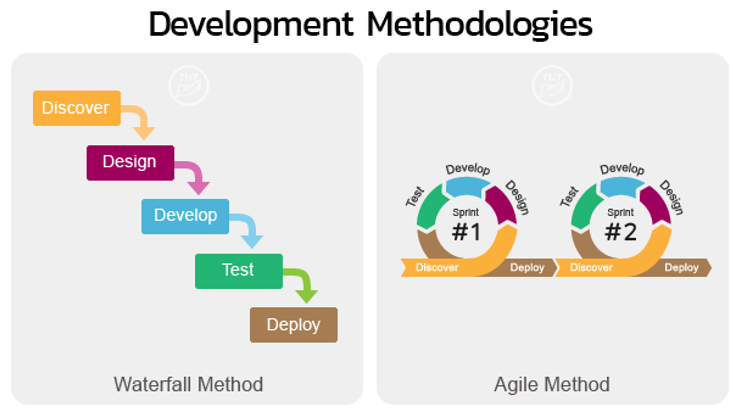
\includegraphics[scale=0.6]{agile}
		\caption{ความแตกต่างระหว่าง Waterfall Method กับ Agile Method}
		\end{figure}
	\FloatBarrier
	\item Scrum (สกรัม) คือการนำแนวคิดในการทำงานแบบ Agile (อไจล์) มาปฏิบัติตามขั้นตอนของสกรัม เพื่อระบุปัญหาที่มีความซับซ้อน เปลี่ยนแปลงบ่อย เพื่อให้สามารถส่งมอบผลิตภัณฑ์ที่ตอบสนองต่อการเปลี่ยนแปลงที่เกิดขึ้นได้อย่างรวดเร็ว
ช่วยให้การพัฒนาผลิตภัณฑ์แบบ Agile มีขั้นตอนการการดำเนินงานและผลลัพธ์ที่ชัดเจน โปร่งใส สามารถตรวจสอบประสิทธิภาพของแต่ละขั้นตอนการดำเนินงาน สามารถปรับปรุงและวัดผลการปรับปรุงที่เกิดขึ้นได้
	\item Kanban ที่มาเริ่มต้นมาจากระบบการทำงานของ Toyota ซึ่งประสบความสำเร็จอย่างมากจนทำให้สามารถผลิตรถออกมาได้ไวกว่าคู่แข่งทั่วโลกจนครองตลาดไปได้มาก สำหรับวงการ Software ได้ถูก David J. Anderson จับนำมาปรับปรุงให้เข้ากับ Software Development เพื่อการพัฒนา Software ได้อย่างรวดเร็วที่สุดด้วยเช่นกัน และสุดท้ายถูกนำไปเป็นส่วนหนึ่งของ Lean Software Development รวมไปถึงถูกจัดให้เป็น Agile อีกแบบหนึ่งนอกเหนือไปจาก Scrum อีกด้วย
Kanban มีกฎอยู่แค่ 3 ข้อ 
	\begin{itemize}[leftmargin=0pt,itemindent=3cm]
		\item Visualize the workflow – แสดง flow การทำงานของระบบให้ออกมาให้เห็นภาพอย่างชัดเจน สามารถบอกได้ว่าขณะนี้งานไปติดขัดที่จุดไหน 			อย่างไรให้ชัดเจน
		\item Limit Work In Progress (WIP) – จุดหลักของ Kanban เลยคือการ limit งานต่อหนึ่งหน่วยย่อย เช่นงานสำหรับ Development ห้ามถือเกิน	 			2 งานเพื่อป้องกันไม่ให้งาน Overload มากเกินไป และจะทำให้สูญเสียเวลาไปมากกว่าที่ควรจะเป็น
		\item Measure the lead time – วัดผลการทำงานและปรับปรุงให้ดียิ่งขึ้นไปอีก ตรงนี้จะเรียกว่า Cycle time หรือค่าเฉลี่ยที่ Card 1 							อันจะอยู่บนบอร์ดตั้งแต่เริ่มต้นไปจนถึงขึ้นบน production จริง
		\end{itemize}
	\end{itemize}
\end{enumerate}

\subsection{Smart Contract \cite{smartcontract}}
\tab Smart Contract หมายถึง กระบวนการทางดิจิทัล ที่กำหนดขั้นตอนการทำธุรกรรมโดยอัตโนมัติไว้ล่วงหน้า โดยไม่ต้องอาศัยตัวกลาง อย่างเช่น ธนาคาร ซึ่งการสร้าง Smart Contract ที่เป็นระบบอัตโนมัติอย่างเต็มรูปแบบ โดยคู่สัญญาทั้งสองฝ่ายจะมีการตกลงกันก่อนหน้านี้ ถึงขั้นตอน กลไก ในการทำรายการธุรกรรมดังกล่าว ซึ่งการพัฒนานี้ส่งผลกระทบต่อรูปแบบธุรกิจแบบดั้งเดิมของธนาคาร

\subsection{Non-Fungible Token (NFT) \cite{nft}}
\tab NFT ย่อมาจาก Non-Fungible Token เป็นชื่อเรียกของ Cryptocurrency ประเภทหนึ่ง เป็นสินทรัพย์ดิจิทัลที่มีเพียงชิ้นเดียวในโลก ไม่สามารถทำซ้ำหรือคัดลอกได้ ต่อให้มีการก๊อบปี้ไป แต่ต้นฉบับของจริงจะมีอยู่เพียงหนึ่งเดียวเท่านั้น ส่วนโทเคน NFT ก็เป็นเหมือนโฉนด เพื่อแสดงความเป็นเจ้าของสินทรัพย์ชิ้นนั้น

\subsection{Asset (สินทรัพย์)  \cite{asset}}
\tab Asset หมายถึง ทรัพยากรที่มีและอยู่ในการควบคุมของกิจการ สินทรัพย์นี้อาจจะเป็นสิ่งที่มีตัวตนหรือไม่มีตัวตนก็ได้ ซึ่งสามารถตีราคามูลค่าเป็นเงินได้ ทรัพยากรดังกล่าวเป็นผล ของ เหตุการณ์ในอดีต ซึ่งกิจการคาดว่าจะได้รับประโยชน์เชิงเศรษฐกิจจากทรัพยากรนั้นในอนาคต

\subsection{Digital Asset (สินทรัพย์ดิจิทัล)  \cite{digital-asset}}
\tab คือ "สิ่งที่มีมูลค่าและเราสามารถเป็นเจ้าของได้ แต่ไม่สามารถแตะต้องได้ทางกายภาพ" สิ่งเหล่านั้นถูกสร้างขึ้นในระบบดิจิทัล และเก็บไว้ในอุปกรณ์อิเล็กทรอนิกส์อย่าง คอมพิวเตอร์ ฮาร์ดแวร์ แล็ปท็อป หรือ อุปกรณ์เก็บข้อมูลต่าง ๆ เป็นต้น

\subsection{พินัยกรรม  \cite{will}}
\tab พินัยกรรม หมายถึง การแสดงเจตนากำหนดการเผื่อตายซึ่งให้มีผลบังคับได้เมื่อถึงแก่ความตาย หรือถ้าเป็นภาษาพูดก็ได้แก่คำสั่งเสียของผู้ตาย โดยในการทำพินัยกรรม กฎหมายกำหนดรูปแบบไว้ 5 แบบด้วยกัน ดังนี้
\begin{enumerate}[label=\thesubsection.\arabic*,leftmargin=0pt,itemindent=2.5cm]
\item พินัยกรรมแบบธรรมดา ผู้ทำต้องทำเป็นหนังสือ คือการพิมพ์ข้อความพินัยกรรมลงในกระดาษ มากน้อยหรือจำนวนกี่แผ่นก็ต้องแล้วแต่เนื้อหาหรือจำนวนทรัพย์สิน   ลงวัน เดือน ปี ที่ทำให้ชัดเจน และผู้ทำต้องลงลายมือชื่อไว้ต่อหน้าพยานอย่างน้อย 2 คน และพยานต้องลงลายมือชื่อรับรองการทำพินัยกรรมในขณะทำด้วย
\item พินัยกรรมแบบเขียนเองทั้งฉบับ ผู้ทำพินัยกรรมจะทำเป็นเอกสารเขียนเองทั้งฉบับก็ได้ แต่ผู้ทำนั้นต้องเขียนพินัยกรรมนั้นด้วยลายมือตนเอง   ลงวัน เดือน ปีที่ทำ และที่สำคัญต้องลงลายมือชื่อผู้ทำด้วย กรณีนี้จะมีพยานมารับรู้การทำพินัยกรรมด้วยหรือไม่มีก็ได้
\item พินัยกรรมแบบเอกสารฝ่ายเมือง เป็นแบบพินัยกรรมที่ต้องอาศัยกระบวนการโดยเฉพาะที่มีเจ้าหน้าที่รัฐเข้ามาเกี่ยวข้อง   ผู้ทำพินัยกรรมต้องไปแจ้งความประสงค์โดยให้ถ้อยคำข้อความของตนแก่เจ้าพนักงานที่เขตหรืออำเภอพร้อมพยานอย่างน้อย 2 คน   เจ้าพนักงานจะอ่านข้อความให้ผู้ทำพินัยกรรมและพยานฟัง เมื่อเห็นว่าถูกต้องครบถ้วนแล้ว ผู้ทำพินัยกรรมพร้อมพยานทั้งสองต้องลงลายมือชื่อไว้   ต่อจากนั้น เจ้าพนักงานจะลงลายมือชื่อ วัน เดือน ปี ที่ทำ พร้อมประทับตราตำแหน่ง
\item พินัยกรรมแบบเอกสารลับ ผู้ทำพินัยกรรมทำพินัยกรรมแล้วปิดผนึก และนำไปที่ที่ทำการอำเภอหรือเขต   ผู้ทำพินัยกรรมต้องลงลายมือชื่อและพยานอีกอย่างน้อย 2 คน และให้ถ้อยคำต่อบุคคลเหล่านั้นว่าเป็นพินัยกรรมของตน   เจ้าหน้าที่จะบันทึกถ้อยคำลง วัน เดือน ปี ที่ทำพินัยกรรมแสดงไว้บนซองและประทับตราตำแหน่งไว้เป็นสำคัญโดยผู้ทำพินัยกรรม   พยานและเจ้าหน้าที่ต้องลงลายมือชื่อไว้หน้าซองตรงที่ปิดผนึก
\item พินัยกรรมแบบทำด้วยวาจา กรณีมีพฤติการณ์พิเศษที่บุคคลไม่สามารถทำพินัยกรรมแบบอื่นที่กล่าวมาข้างต้น เช่น การตกอยู่ในภยันตรายใกล้ความตาย หรืออยู่ในระหว่างสงคราม หรือเกิดมีโรคระบาด   เราสามารถทำพินัยกรรมแบบทำด้วยวาจาก็ได้ โดยผู้ทำพินัยกรรมต้องแสดงเจตนาทำพินัยกรรมต่อหน้าพยานอย่างน้อย 2 คนพร้อมกัน   พยานต้องรับฟังข้อความนั้นแล้วไปแจ้งต่อทางราชการโดยเร็วที่สุด ทั้งยังต้องแจ้งวัน เดือน ปี สถานที่ทำพินัยกรรมและพฤติการณ์พิเศษนั้นด้วย   เจ้าพนักงานต้องจดข้อความที่พยานแจ้งไว้ และพยาน 2 คนนั้นต้องลงลายมือชื่อไว้
\end{enumerate}
ข้อจำกัดและข้อควรระวังในการทำพินัยกรรม
\begin{enumerate}[label=\arabic*.,leftmargin=0pt,itemindent=2.5cm]
\item พินัยกรรมเป็นนิติกรรมที่ต้องทำตามแบบที่กำหนดเท่านั้น
\item ต้องเขียน วัน เดือน ปี ลงลายมือชื่อทั้งผู้ทำพินัยกรรมและผู้ที่เป็นพยาน
\item ผู้ที่เป็นพยานจะต้องไม่เป็นผู้เยาว์หรือผู้หย่อนความสามารถ และต้องไม่เป็นผู้มีส่วนได้เสียในกองมรดกนั้นด้วย
\item ผู้ทำพินัยกรรมต้องมีอายุ 15 ปีบริบูรณ์ขึ้นไป
\item พินัยกรรมควรจะตั้งผู้จัดการมรดกโดยสามารถระบุผู้ทำหน้าที่ผู้จัดการมรดกที่เจ้ามรดกไว้ใจลงในพินัยกรรมไปได้เลย
\item สิทธิ หน้าที่ และความรับผิดชอบ ก็สามารถกำหนดในพินัยกรรมได้
\item ทรัพย์สินที่ระบุในพินัยกรรมต้องเป็นทรัพย์สินหรือสิทธิของผู้ทำพินัยกรรมเท่านั้น ทั้งต้องแยกสินส่วนตัวออกจากสินสมรสด้วย
\item เงินประกันชีวิต เงินบำเหน็จตกทอด เงินมีบำนาญตกทอด เงินฌาปนกิจสงเคราะห์ตกทอด ไม่อาจเป็นมรดกที่ระบุลงในพินัยกรรมได้ เพราะไม่ใช่ทรัพย์ที่เจ้ามรดกมีอยู่ก่อนตาย
\section{งานวิจัยที่เกี่ยวข้อง}
\tab ในส่วนนี้เป็นการสรุปเนื้อหาโดยรวมของงานวิจัยที่เกี่ยวข้องกับการพัฒนาโครงงาน Will Chain Web application ที่มีการใช้งานในส่วนของ Digital Asset คือ CryptoWill
\subsection{CryptoWill  \cite{cryptowill}}
\tab โปรเจคนี้ได้อธิบายวิธีการทำระบบ CryptoWill ด้วยการให้ user ทำการเลือกเหรียญที่ต้องการทำ Smart Contract ที่ต้องการส่งให้ทายาทและหลังจากนั้นตัวระบบจะทำการให้กำหนดเวลาของการ contract นี้จะส่งต่อเมื่อไหร่ อย่างเช่น ถ้าตั้ง 2 ปี ผู้ใช้งานจะต้องมาก่อนเวลาที่จะเกิด contract นี้ โดยรูปแบบของการทำจะมีวิธีการดำเนินการดังรูป

\begin{figure}[h]
	\centering
	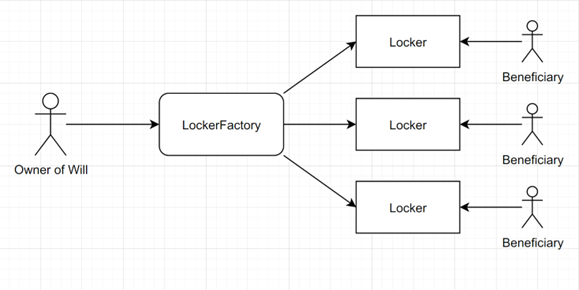
\includegraphics[scale=0.6]{CryptoWill}
	\caption{ภาพแสดงหลักการทำงานของโปรเจค CryptoWill}
\end{figure}

โดยเจ้าของพินัยกรรมจะทำพินัยกรรมและจะเก็บสินทรัพย์ไว้ใน blockchain และหลังจากนั้นจะส่งต่อให้ทายาทไปเมื่อถึงเวลาของพินัยกรรม
\end{enumerate}
\section{เทคนิคและเทคโนโลยีที่ใช้}

\subsection{Ethereum Chain  \cite{eth}} 
\tab Ethereum คือแพลตฟอร์มบน Blockchain Network ที่่ทํางานด้วย Smart Contract มีลักษณะแพลตฟอร์มเป็นรูปแบบ Decentralized Platform แบบ Open Source ทําให้นักพัฒนาสามารถเข้ามาพัฒนา แก้ไข หรือดัดแปลงโค้ดได้ทุกคน พร้อมทั้งกําหนดเงื่อนไขต่าง ๆ สําหรับนําไปใช้งานบน Blockchain โดยมี Smart Contract ดําเนินการและระบบจะทํางานตามเงื่อนไขโปรแกรมที่กําหนดมา ทําให้ผู้ใช้งาน Blockchain ของ Ethereum ทําธุรกรรมได้ โดยไม่ต้องผ่านตัวกลางอื่น

\subsection{GitHub  \cite{github}}
\tab Git คือ Version Control ที่ถูกพัฒนาขึ้นมาเพื่อใช้ใ้นกระบวนการพัฒนาซอฟต์แวร์ คือ ระบบที่ถูกพัฒนาขึ้นมาเพื่อใช้สำหรับการติิดตาม ตรวจสอบ การพัฒนา แก้ไข Source Code ไฟล์ต่าง ๆ ในขั้นตอนการพัฒนา ที่สามารถตรวจสอบ ได้ทุกตัวอักษร ทุกบรรทัด ทุกไฟล์์ที่มีีการแก้ไข และยังมีคุณณลักษณะที่สนับสนุนการทำงานแบบ Agile อีกด้วย จึงทำให้เราสามารถทำงานได้อย่างมีประสิทธิภาพมากยิ่งขึ้น

\subsection{MetaMask \cite{metamask}}
\tab MetaMask หรือ MetaMask Wallet กระเป๋าเงินสินทรัพย์ดิจิทัล เป็น Wallet สำหรับเก็บ Cryptocurrency บนระบบนิเวศของ Ethereum ทุกชนิด ในกลุ่ม ERC-20 ซึ่ง Metamask พัฒนาโดยบริษัท ConsenSys โดยมีผู้ก่อตั้งคือ Joseph Lubin เมื่อปี 2016 (Joseph Lubin ยังเป็นผู้ร่วมก่อตั้ง Ethereum และ เคยยังเคยเป็น Speaker ในงาน Techsauce Global Summit)

\subsection{NestJS \cite{nestjs}}
\tab NestJS เป็น Framework สำหรับ Build Node.js ในฝั่ง Server-side Applications โดยสนันสนุนการทำงานแบบ
	\begin{itemize}[leftmargin=0pt,itemindent=2.5cm]
		\item TypeScript เต็มรูปแบบ
		\item OOP (Object Oriented Programming)
		\item FP (Functional Programming)
		\item FRP (Functional Reactive Programming)
	\end{itemize}

\subsection{Next.js \cite{nextjs}}
\tab Next.js คือ JavaScript webapps framework ถูกสร้างขึ้น on top จาก library ดัง ๆ อย่าง React, Webpack, และ Babel และมีจุดเด่นที่ server-side rendering ที่สามารถ render หน้าเว็บบน server แทนที่จะ render บน browser ได้ จึงทำให้ข้อมูลที่ส่งให้ฝั่ง client นั้นถูก render เสร็จเรียบร้อยแล้ว ทำให้ฝั่ง client สามารถนำไปแสดงผลได้ทันที

\subsection{Solidity \cite{solidity}}
\tab Solidity คือภาษาสำหรับการสร้าง Smart Contract เป็นภาษาที่ได้รับอิทธิพลมาจาก C ++, Python และ JavaScript ที่สำคัญเลยก็คือเป็นภาษาชนิดที่ statically typed และเป็นภาษาแบบ Object Oriented (OO) เพราะว่ามีคุณสมบัติของการสืบทอดและการทำ struct เป็นต้น

\subsection{TypeScript \cite{typescript}}
\tab TypeScript เป็นภาษาโปรแกรมที่รวมความสามารถที่ ES2015 เองมีอยู่ สิ่งที่เพิ่มขึ้นมาคือสนับสนุน Type System รวมถึงคุณสมบัติอื่นๆที่เพิ่มมากขึ้น เช่น Enum และความสามารถที่เพิ่มขึ้นของการโปรแกรมเชิงวัตถุ TypeScript นั้นเป็น transpiler เหมือน Babel นั่นหมายความว่าตัวแปลภาษาของ TypeScript จะแปลโค๊ดที่เราเขียนให้เป็น JavaScript อีกทีนึง จึงมั่นใจได้ว่าผลลัพธ์สุดท้ายจะสามารถใช้งานได้บนเว็บเบราเซอร์ทั่วไป

\subsection{Web3.js \cite{web3js}}
\tab Web3.js เป็น JavaScript API ที่ทําให้ส่วนติดต่อผู้ใช้งานสามารถติดต่อและเรียกใช้ฟังก์ชันจากฝั่งของ Ethereum ได้ โดย Web3.js สามารถส่ง API ไปติดต่อกับฝั่ง Smart Contract ให้สร้าง Transaction สําหรับเรียกใช้ Methods หรือ Get ค่าตัวแปรต่าง ๆ บน Smart Contract ที่อยู่บน Ethereum Blockchain ได้
\clearpage

\subsection{Hardhat \cite{hardhat}}
\tab Hardhat เป็น Development Environment ที่ทำให้เราสามารถพัฒนาตัว Smart Contract ได้โดย Hardhat สามารถทำ Compile, Deploy, Test, Debug ของตัว Smart contract และ สามารถ Test ตัว Smart Contract ได้บน Local Network ตัวเองได้

\subsection{Pinata \cite{pinata}}
\tab Pinata เป็น Development Environment ที่ทำให้เราสามารถพัฒนาตัว Smart Contract ได้โดย Hardhat สามารถทำ Compile, Deploy, Test, Debug ของตัว Smart contract และ สามารถ Test ตัว Smart Contract ได้บน Local Network ตัวเองได้

\subsection{IPFS \cite{ipfs}}
\tab IPFS เป็นเครือข่ายกระจายอำนาจแบบเพียร์ทูเพียร์ที่ช่วยให้ผู้ใช้สำรองไฟล์และเว็บไซต์โดยการโฮสต์ไว้บนโหนดจำนวนมาก ถูกสร้างขึ้นโดย Protocol Labs เป็นบริการที่อาศัยเครือข่ายคอมพิวเตอร์แบบกระจายที่โฮสต์เนื้อหา เช่น หน้าเว็บ ไฟล์ และแอปที่มิเรอร์ ซึ่งทั้งหมดนี้คุณสามารถดึงขึ้นมาได้โดยการป้อนลิงก์
Pinatas เป็นบริการโฮสต์ NFT ที่ใช้ IPFS เพื่อสำรองข้อมูลของสะสม crypto สำหรับคู่ค้าเช่น Rarible และ Sorare


\chapter{การออกแบบและวิธีการดำเนินงาน}
\tab เอกสารรายงานบทนี้จะกล่าวถึงระบบการทำงานของโครงงาน รวมถึงแผนภาพต่าง ๆ ที่ใช้อธิบายการทำงานในส่วนต่าง ๆ ของระบบ การออกแบบส่วนติดต่อผู้ใช้งาน (User Interface) ไดอะแกรมของระบบ รวมถึงขั้นตอนและวิธีการดำเนินงาน
\section{ระบบการทำงาน}
\subsection{ภาพรวมของระบบ}
\tab โดยภาพรวมของ Will Chain (Web application) จะประกอบไปด้วย 3 ส่วนหลักดังนี้
	\begin{figure}[h]
		\centering
		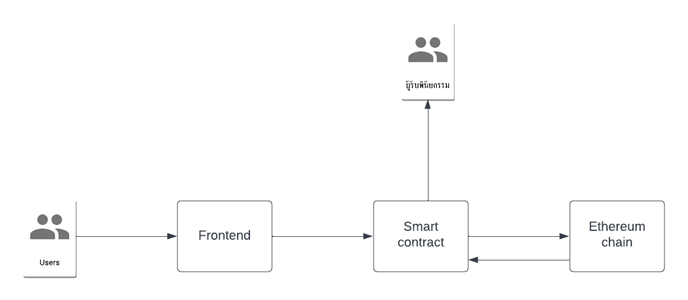
\includegraphics[scale=0.8]{Overall_system}
		\caption{ภาพรวมแสดงการทำงานของระบบ}
	\end{figure}
	\begin{itemize}[leftmargin=0pt,itemindent=2.5cm]
		\item ส่วนติดต่อผู้ใช้งานหรือ Frontend จะเป็นส่วนที่ผู้ใช้งานเห็น และใช้งาน
		\item Smart Contract จะเป็นส่วนที่ควบคุมการทำงานของระบบทั้งหมด โดยที่ผู้ใช้งานจะเข้าใช้งานผ่านทาง Frontend และจะส่งชุดคำสั่งมาเพื่อที่จะสั่งให้ Smart Contract นั้นทำงาน และจะส่งข้อมูลไปเก็บใน Blockchain ต่อไป
		\item Ethereum chain สำหรับเก็บข้อมูลการใช้งานของผู้ใช้งาน
	\end{itemize}

\subsection{User Journey}
	\begin{figure}[h]
		\centering
		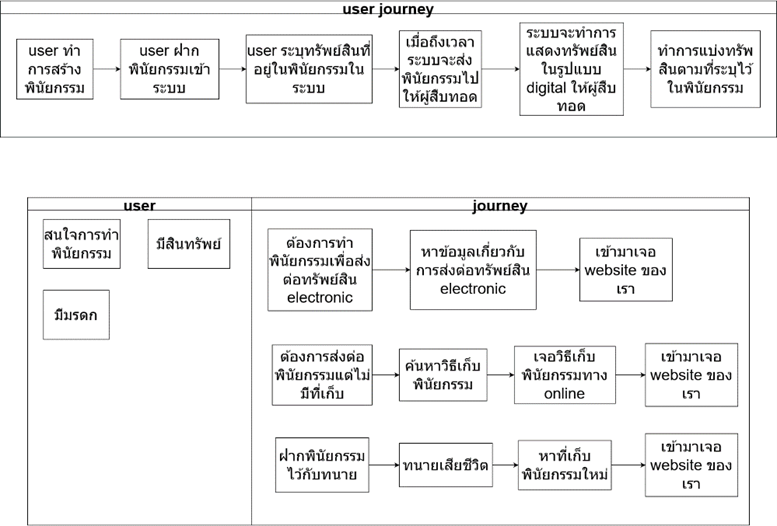
\includegraphics[scale=0.8]{UserJourney}
		\caption{แสดง User Journey}
	\end{figure}
\FloatBarrier
\hfill\\
\hfill\\
\hfill\\
\section{Cryptocurrency Wallet}
\tab ในการออกแบบระบบการทํางานของ Will Chain web application ได้เลือกใช้งาน Cryptocurrency Wallet ที่สามารถเชื่อมต่อกับ
Ethereum chain ได้ เพื่อที่จะทําให้สามารถทดสอบ และใช้งานจริงได้บน Ethereum chain โดย Cryptocurrency Wallet โดยเลือกใช้เป็น Metamask Wallet

\section{Diagram Unified Modelling Language (UML)}
\tab หลังจากได้เขียนความต้องการ และฟังก์ชันแล้ว จึงทำการออกแบบและเขียนแผนภาพไดอะแกรมต่าง ๆ เพื่อให้สามารถเข้าใจระบบการทำงานมากยิ่งขึ้น โดยมีรายละเอียดดังนี้

\subsection{แผนภาพ Use Case Diagram}
	\begin{figure}[!htb]
		\centering
		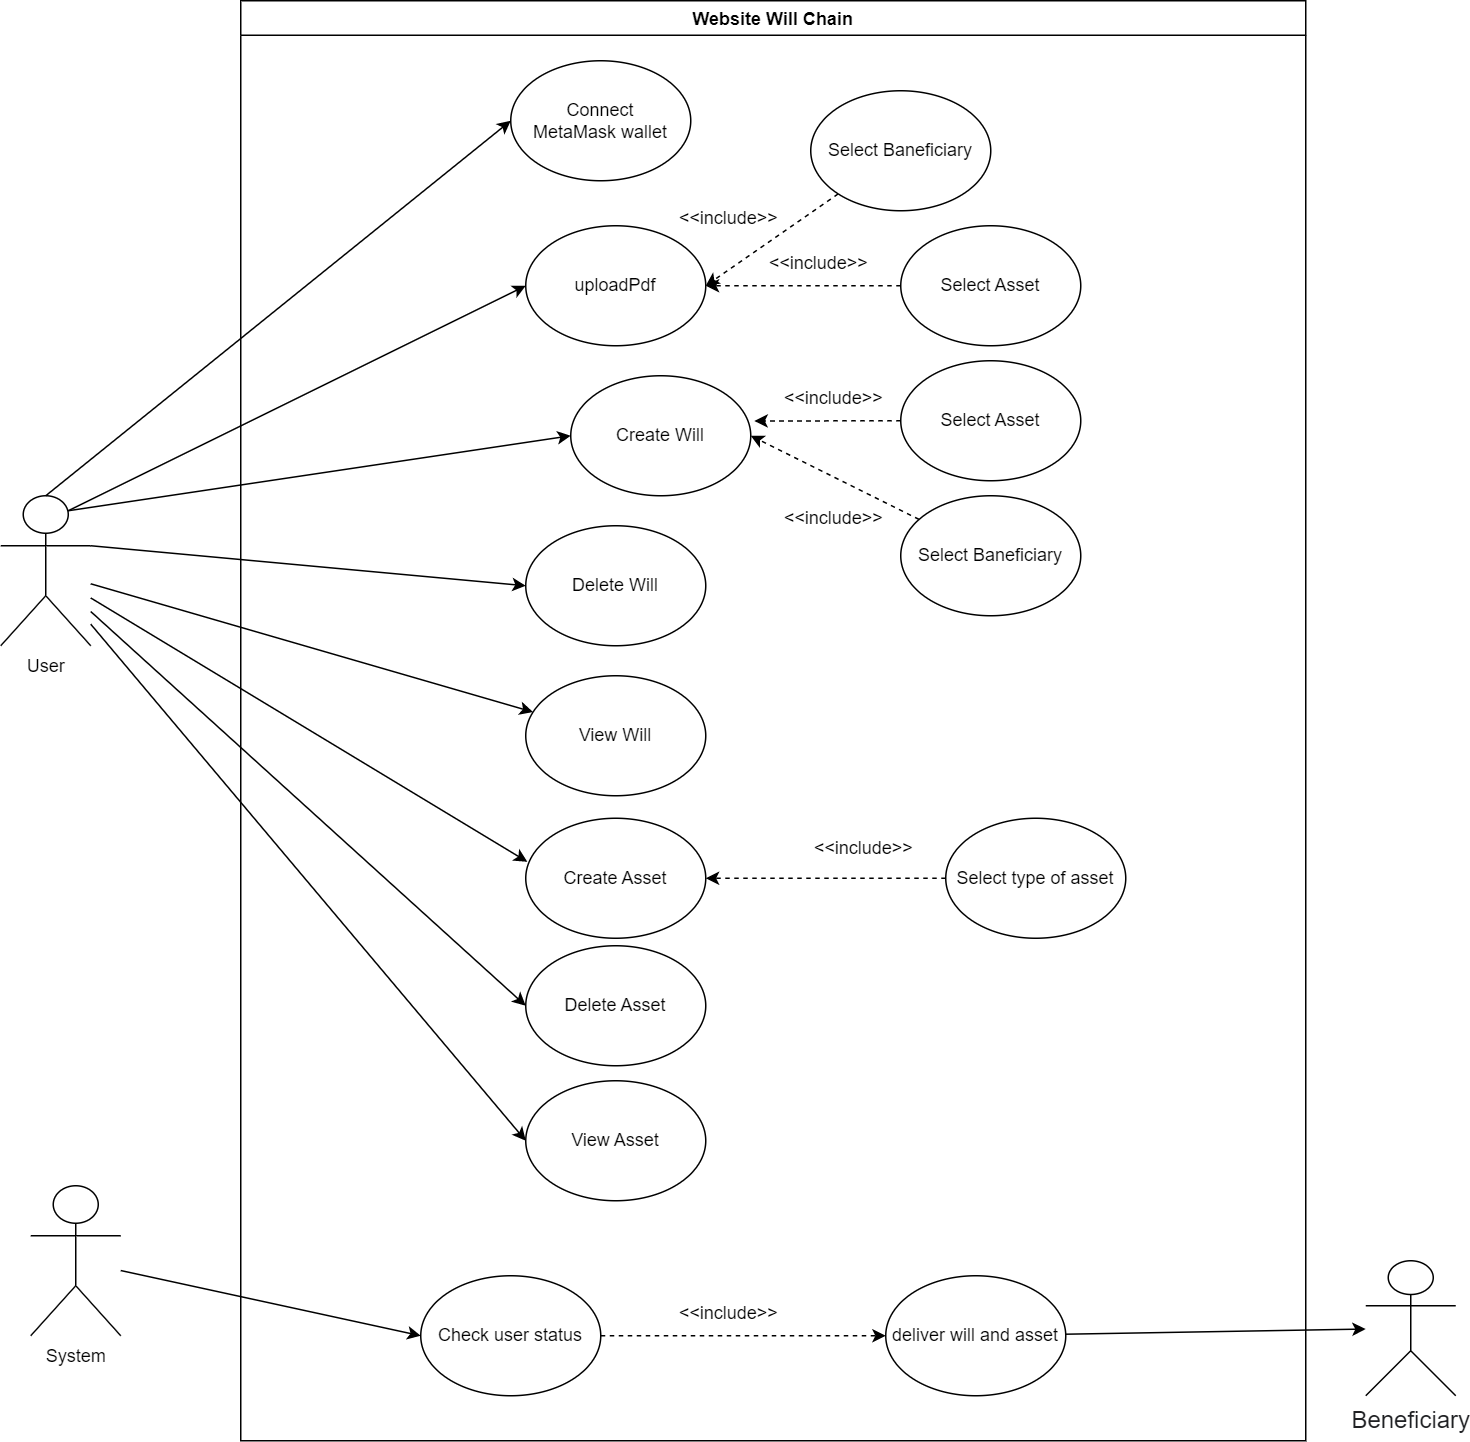
\includegraphics[scale=0.5]{UseCaseDiagram}
		\caption{แสดงการทำงานของระบบทั้งหมด Use Case Diagram}
	\end{figure}
\FloatBarrier
\tab จากรูปแสดง Use Case แสดงการทำงานของระบบทั้งหมดโดยจะมีผู้ใช้งาน (User) ที่ต้องการฝากพินัยกรรมไว้ในระบบทำการใช้งานระบบผ่าน platform ของ Will Chain Web application  โดยผู้ใช้งานจำเป็นต้องเชื่อมต่อกระเป๋าเงินอิเล็กทรอนิกส์ของ meta mask ก่อนหลังจากนั้นจึงจะสามารถ สร้าง,ลบหรือ upload พินัยกรรมพร้อมทั้งมีระบบจัดการทรัพย์สินที่ผู้ใช้แนบไว้พร้อมกับพินัยกรรม และจะมีระบบที่ทำการตรวจสอบสถานะของผู้ใช้งานเพื่นที่จะทำการส่งผ่านพินัยกรรมไปยังผู้รับผลประโยชน์เมื่อถึงเวลา   จากแผนภาพ Use Case Diagram ตามรูปที่ สามารถอธิบายรายละเอียดการทํา งานของแต่ละ Use Case ได้ดังต่อไปนี้ โดยจะกล่าวถึงในหัวข้อ Use Case Narrative ถัดไป
\clearpage
\subsection{Use Case Narrative}
\begin{enumerate}[label=\thesubsection.\arabic*,leftmargin=0pt,itemindent=1.25cm]
\item Use Case Connect Wallet
	\begin{table}[h]
\centering
\caption{ตารางแสดงรายละเอียดของ Use Case Connect MetaMask Wallet}
\begin{tabularx}{\textwidth}{|l|X|X|} 
\hline
Use Case Name:     & \multicolumn{2}{l|}{Connect MetaMask wallet}                                                                                                                                                                                                                       \\ 
\hline
Actors:            & \multicolumn{2}{l|}{User}                                                                                                                                                                                                                                          \\ 
\hline
Pre-Condition:     & \multicolumn{2}{l|}{User ต้องทำการสร้างกระเป๋าเงิน
  MetaMask}                                                                                                                                                                                                     \\ 
\hline
Post-Condition:    & \multicolumn{2}{l|}{กระเป๋าเงินเชื่อมต่อกับ
  platform}                                                                                                                                                                                                            \\ 
\hline
Brief Description: & User                                                                                                        & System                                                                                                                                               \\ 
\hline
Flow of Event:     & \begin{tabular}[c]{@{}l@{}}1.เลือกเมนู Connect Wallet \\\\3.ยืนยันการเชื่อมต่อ MetaMask Wallet\end{tabular} & \begin{tabular}[c]{@{}l@{}}~ ~ ~ ~ \\2.รอผู้ใช้งานเลือก Account และยืนยันการเชื่อมต่อ \\~ ~\\4.เชื่อมต่อ MataMask Wallet กับ Platform\end{tabular}  \\ 
\hline
Exception:         & ~                                                                                                           &                                                                                                                                                      \\
\hline
\end{tabularx}
\end{table}
\FloatBarrier
\item Use Case Create Will
	\begin{table}[h]
\centering
\caption{ตารางแสดงรายละเอียดของ Use Case Create Will}
\begin{tabularx}{\textwidth}{|l|X|X|} 
\hline
Use Case Name:     & \multicolumn{2}{l|}{Create Will}                                                                                                                                                                                        \\ 
\hline
Actors:            & \multicolumn{2}{l|}{User}                                                                                                                                                                                               \\ 
\hline
Pre-Condition:     & \multicolumn{2}{l|}{User ต้องทำการเชื่อมบัญชีกับกระเป๋าเงิน
  meta mask}                                                                                                                                                \\ 
\hline
Post-Condition:    & \multicolumn{2}{l|}{พินัยกรรมถูกบันทึกเข้าระบบ}                                                                                                                                                                         \\ 
\hline
Brief Description: & User                                                                                           & System                                                                                                                 \\ 
\hline
Flow of Event:     & \begin{tabular}[c]{@{}l@{}}1.เลือกเมนู Create Will \\~\\3.ยืนยันการสร้างพินัยกรรม\end{tabular} & \begin{tabular}[c]{@{}l@{}}~\\2.รอผู้ใช้งานกรอกรายละเอียดพินัยกรรมให้เสร็จ \\~\\4.บันทึกพินัยกรรมเข้าสู่ระบบ\end{tabular}  \\ 
\hline
Exception:         & ~                                                                                              &                                                                                                                        \\
\hline
\end{tabularx}
\end{table}
\FloatBarrier
\item Use Case View Will
	\begin{table}[h]
\centering
\caption{ตารางแสดงรายละเอียดของ  Use Case View Will}
\begin{tabularx}{\textwidth}{|l|X|X|} 
\hline
Use Case Name:     & \multicolumn{2}{l|}{View Will}                                                                                                                                                                                                                  \\ 
\hline
Actors:            & \multicolumn{2}{l|}{User}                                                                                                                                                                                                                       \\ 
\hline
Pre-Condition:     & \multicolumn{2}{l|}{User ต้องมีพินัยกกรรมที่ถูกสร้างไว้เรียบร้อยแล้ว}                                                                                                                                                                           \\ 
\hline
Post-Condition:    & \multicolumn{2}{l|}{ระบบทำการแสดงพินัยกรรมในระบบให้
  User}                                                                                                                                                                                     \\ 
\hline
Brief Description: & User                                                                                                              & System                                                                                                                      \\ 
\hline
Flow of Event:     & \begin{tabular}[c]{@{}l@{}}1.เลือกเมนู View Will \\\\3.เลือกพินัยกรรมที่อยู่ในระบบที่ต้องการดู \\~ ~\end{tabular} & \begin{tabular}[c]{@{}l@{}}2.ระบบทำการแสดงพินัยกรรมที่ถูกบันทึกในระบบ  \\\\4.ทำการแสดงพินัยกรรมที่ User เลือก\end{tabular}  \\ 
\hline
Exception:         & \multicolumn{2}{l|}{~}                                                                                                                                                                                                                          \\
\hline
\end{tabularx}
\end{table}
\FloatBarrier
\clearpage
\item Use Case Upload Will
\begin{table}[h]
	\centering
	\caption{ตารางแสดงรายละเอียดของ Use Case Upload Will}
	\begin{tabularx}{\textwidth}{|l|X|X|} 
	\hline
	Use Case Name:     & \multicolumn{2}{l|}{Upload Will}                                                                                                                                           \\ 
	\hline
	Actors:            & \multicolumn{2}{l|}{User}                                                                                                                                                  \\ 
	\hline
	Pre-Condition:     & \multicolumn{2}{l|}{User ต้องทำการเชื่อมบัญชีกับกระเป๋าเงิน
	  meta mask}                                                                                                   \\ 
	\hline
	Post-Condition:    & \multicolumn{2}{l|}{พินัยกรรมถูกบันทึกเข้าระบบ}                                                                                                                            \\ 
	\hline
	Brief Description: & User                                                                                           & System                                                                    \\ 
	\hline
	Flow of Event:     & \begin{tabular}[c]{@{}l@{}}1.เลือกเมนู Upload Will \\2.ยืนยันการ Upload พินัยกรรม\end{tabular} & \begin{tabular}[c]{@{}l@{}}\\\\3.บันทึกพินัยกรรมเข้าสู่ระบบ\end{tabular}  \\ 
	\hline
	Exception:         & ~                                                                                              &                                                                           \\
	\hline
\end{tabularx}
\end{table}
\FloatBarrier
\item Use Case Delete Will
	\begin{table}[h]
\centering
\caption{ตารางแสดงรายละเอียดของ Use Case Delete Will}
\begin{tabularx}{\textwidth}{|l|X|X|} 
\hline
Use Case Name:     & \multicolumn{2}{l|}{Delete Will}                                                                                                                                                                                                                                                          \\ 
\hline
Actors:            & \multicolumn{2}{l|}{User}                                                                                                                                                                                                                                                                 \\ 
\hline
Pre-Condition:     & \multicolumn{2}{l|}{User ต้องมีพินัยกกรมที่ถูกสร้างไว้เรียบร้อยแล้ว}                                                                                                                                                                                                                      \\ 
\hline
Post-Condition:    & \multicolumn{2}{l|}{พินัยกรรมถูกลบออกจากระบบ}                                                                                                                                                                                                                                             \\ 
\hline
Brief Description: & User                                                                                                                                                       & System                                                                                                                       \\ 
\hline
Flow of Event:     & \begin{tabular}[c]{@{}l@{}}1.เลือกเมนู Delete Will \\\\3.เลือกพินัยกรรมที่อยู่ในระบบ \\4.ลบพินัยกรรมในระบบ \\5.ยืนยันการลบพินัยกรรมในระบบ \\~\end{tabular} & \begin{tabular}[c]{@{}l@{}}\\2.ระบบทำการแสดงพินัยกรรมที่ถูกบันทึกในระบบ  \\\\\\\\6. ทำการนำพินัยกรรมออกจากระบบ\end{tabular}  \\ 
\hline
Exception:         & \multicolumn{2}{l|}{~}                                                                                                                                                                                                                                                                    \\
\hline
\end{tabularx}
\end{table}
\FloatBarrier
\item Use Case View Beneficiary
\begin{table}[h]
\centering
\caption{ตารางแสดงรายละเอียดของ Use Case View Beneficiary}
\begin{tabularx}{\textwidth}{|l|X|X|} 
\hline
Use Case
  Name:     & \multicolumn{2}{l|}{View Beneficiary}                                                                                                         \\ 
\hline
Actors:              & \multicolumn{2}{l|}{User}                                                                                                                      \\ 
\hline
Pre-Condition:       & \multicolumn{2}{l|}{ระบบต้องมีการเพิ่ม beneficiary แล้ว}                                                                           \\ 
\hline
Post-Condition:      & \multicolumn{2}{l|}{ระบบทำการแสดง beneficiary}                                                                                             \\ 
\hline
Brief
  Description: & User  & System                                                                                                                                   \\ 
\hline
Flow of Event:     & \begin{tabular}[c]{@{}l@{}}1.เลือกพินัยกรรมที่ต้องการดู \\~\\3.เลือกเมนู View Baneficiary\end{tabular} & \begin{tabular}[c]{@{}l@{}}~\\2.ระบบทำการแสดงพินัยกรรมที่ถูกบันทึกในระบบ  \\~\\4.ระบบจะทำการแสดง Beneficiary ของพินัยกรรม\end{tabular}  \\ 
\hline
Exception:           & \multicolumn{2}{l|}{~}                                                                                                                           \\
\hline
\end{tabularx}
\end{table}
\FloatBarrier
\clearpage
\item Use Case Set Beneficiary
\begin{table}[h]
\centering
\caption{ตารางแสดงรายละเอียดของ Use Case Set Beneficiary}
\begin{tabularx}{\textwidth}{|l|X|X|} 
\hline
Use Case
  Name:     & \multicolumn{2}{l|}{Set Beneficiary}                                                                                                         \\ 
\hline
Actors:              & \multicolumn{2}{l|}{User}                                                                                                                      \\ 
\hline
Pre-Condition:       & \multicolumn{2}{l|}{ระบบต้องสร้างพินัยกรรมก่อน}                                                                           \\ 
\hline
Post-Condition:      & \multicolumn{2}{l|}{ผู้รับพินัยกรรมถูกบันทึกเข้าสู่ระบบ}                                                                                             \\ 
\hline
Brief
  Description: & User  & System                                                                                                                                   \\ 
\hline
Flow of Event:     & \begin{tabular}[c]{@{}l@{}}1.เลือกพินัยกรรมที่ต้องการเพิ่ม beneficiary \\~\\3.เลือกเมนู Set Baneficiary\end{tabular} & \begin{tabular}[c]{@{}l@{}}~\\2.ระบบทำการแสดงพินัยกรรมที่ถูกบันทึกในระบบ  \\~\\4.ระบบจะทำการบันทึก Beneficiary ของพินัยกรรม\\เข้าสู่ระบบ\end{tabular}  \\ 
\hline
Exception:           & \multicolumn{2}{l|}{~}                                                                                                                           \\
\hline
\end{tabularx}
\end{table}
\FloatBarrier
\item Use Case View Asset
\begin{table}[h]
	\centering
	\caption{ตารางแสดงรายละเอียดของ Use Case View Asset}
	\begin{tabularx}{\textwidth}{|l|X|X|} 
	\hline
	Use Case Name:     & \multicolumn{2}{l|}{View Asset}                                                                                                                                           \\ 
	\hline
	Actors:            & \multicolumn{2}{l|}{User}                                                                                                                                                  \\ 
	\hline
	Pre-Condition:     & \multicolumn{2}{l|}{ระบบต้องมีการเพิ่ม Asset แล้ว}                                                                                                   \\ 
	\hline
	Post-Condition:    & \multicolumn{2}{l|}{ระบบทำการแสดง Asset}                                                                                                                            \\ 
	\hline
	Brief Description: & User                                                                                           & System                                                                    \\ 
	\hline
	Flow of Event:     & \begin{tabular}[c]{@{}l@{}}1.เลือกพินัยกรรมที่ต้องการดู \\~\\3.เลือกเมนู View Asset\end{tabular} & \begin{tabular}[c]{@{}l@{}}~\\2.ระบบทำการแสดงพินัยกรรมที่ถูกบันทึกในระบบ  \\~\\4.ระบบจะทำการแสดง Asset ของพินัยกรรม\end{tabular}  \\ 
	\hline
	Exception:         & ~                                                                                              &                                                                           \\
	\hline
\end{tabularx}
\end{table}
\FloatBarrier
\item Use Case Add Asset
\begin{table}[h]
	\centering
	\caption{ตารางแสดงรายละเอียดของ Use Case Add Asset}
	\begin{tabularx}{\textwidth}{|l|X|X|} 
	\hline
	Use Case Name:     & \multicolumn{2}{l|}{Add Asset}                                                                                                                                           \\ 
	\hline
	Actors:            & \multicolumn{2}{l|}{User}                                                                                                                                                  \\ 
	\hline
	Pre-Condition:     & \multicolumn{2}{l|}{User ต้องทำการ upload พินัยกรรมเข้าสู้ระบบ}                                                                                                   \\ 
	\hline
	Post-Condition:    & \multicolumn{2}{l|}{พินัยกรรมถูกบันทึกเข้าระบบ}                                                                                                                            \\ 
	\hline
	Brief Description: & User                                                                                           & System                                                                    \\ 
	\hline
	Flow of Event:     & \begin{tabular}[c]{@{}l@{}}1.เลือกเมนู Add Asset \\2.ทำการ upload สินทรัพย์\end{tabular} & \begin{tabular}[c]{@{}l@{}}\\\\3.บันทึกสินทรัพย์ไว้ในพินัยกรรม\end{tabular}  \\ 
	\hline
	Exception:         & ~                                                                                              &                                                                           \\
	\hline
\end{tabularx}
\end{table}
\FloatBarrier
\clearpage
\item Use Case Check User Status
\begin{table}[h]
\centering
\caption{ตารางแสดงรายละเอียดของ Use Case Check User Status}
\begin{tabularx}{\textwidth}{|l|X|X|} 
\hline
Use Case
  Name:     & \multicolumn{2}{l|}{Check user
  status}                                                                                                         \\ 
\hline
Actors:              & \multicolumn{2}{l|}{Controller}                                                                                                                      \\ 
\hline
Pre-Condition:       & \multicolumn{2}{l|}{ระบบต้องทำการเชื่อม
  API กับเว็บไซต์กรมการปกครอง}                                                                           \\ 
\hline
Post-Condition:      & \multicolumn{2}{l|}{ระบบทำการตรวจสอบสถาณะของ
  User}                                                                                             \\ 
\hline
Brief
  Description: & User  & System                                                                                                                                   \\ 
\hline
Flow of Event:     & \begin{tabular}[c]{@{}l@{}}1.Controller ตรวจสอบสถาณะของ User \\2.ทำการ active will เพื่อดำเนินการส่งไปหา \\  beneficiary\end{tabular} & \begin{tabular}[c]{@{}l@{}}~\\ \\  \\ 3.ระบบทำการเปลี่ยนสถานะของพินัยกรรม \\ และส่งไปหาผู้รับพินัยกรรม\end{tabular}  \\ 
	
\hline
Exception:           & \multicolumn{2}{l|}{~}                                                                                                                           \\
\hline
\end{tabularx}
\end{table}
\FloatBarrier
\item Use Case Active Will
\begin{table}[h]
\centering
\caption{ตารางแสดงรายละเอียดของ Use Case Active Will}
\begin{tabularx}{\textwidth}{|l|X|X|} 
\hline
Use Case
  Name:     & \multicolumn{2}{l|}{ Active Wil}                                                                                                         \\ 
\hline
Actors:              & \multicolumn{2}{l|}{Controller}                                                                                                                      \\ 
\hline
Pre-Condition:       & \multicolumn{2}{l|}{ระบบต้องเช็คสถานะ User Status เป็น Active}                                                                           \\ 
\hline
Post-Condition:      & \multicolumn{2}{l|}{ระบบทำให้พินัยกรรมดำเนินการส่งต่อไปหา Beneficiary}                                                                                             \\ 
\hline
Brief
  Description: & User  & System                                                                                                                                   \\ 
\hline
Flow of Event:     & \begin{tabular}[c]{@{}l@{}}1.ทำการดำเนินการส่งพินัยกรรม \\ตามเลขบัตรประชาชนที่กำหนด  \\~ ~\end{tabular} & \begin{tabular}[c]{@{}l@{}}2.ทำการส่งพินัยกรรมจากระบบไปหา Beneficiary \end{tabular}  \\ 
\hline
Exception:           & \multicolumn{2}{l|}{~}                                                                                                                           \\
\hline
\end{tabularx}
\end{table}
\FloatBarrier
\clearpage
\item Use Case Claim Will
	\begin{table}[h]
\caption{ตารางแสดงรายละเอียดของ Use Case Claim Will}
\begin{tabularx}{\textwidth}{|l|X|X|} 
\hline
Use Case
  Name:     & \multicolumn{2}{l|}{Claim Will}                                                                                                                                                                                       \\ 
\hline
Actors:              & \multicolumn{2}{l|}{User}                                                                                                                                                                                                         \\ 
\hline
Pre-Condition:       & \multicolumn{2}{l|}{ระบบทำการแจ้งเตือนว่าผู้ทำพินัยกรรมเสียชีวิตแล้ว}                                                                                                                                                                           \\ 
\hline
Post-Condition:      & \multicolumn{2}{l|}{ผู้รับผลประโยชน์เข้ามารับพินัยกรรมและสินทรัพย์}                                                                                                                                           \\ 
\hline
Brief
  Description: & User  & System                                                                                                                                                                                                                      \\ 
\hline
Flow of Event:     & \begin{tabular}[c]{@{}l@{}}1.เลือกเมนู Claim Will \\\\3.เลือกพินัยกรรมในระบบที่สามารถรับได้ \\~ ~\end{tabular} & \begin{tabular}[c]{@{}l@{}}2.ระบบทำการแสดงพินัยกรรมที่ผู้รับผลประโยชน์\\สามารถรับได้  \\\\4.ทำการส่งพินัยกรรมและสินทรัพย์\\ให้ผู้รับผลประโยชน์\end{tabular}  \\ 
\hline
Exception:           & \multicolumn{2}{l|}{~}                                                                                                                                                                                                              \\
\hline
\end{tabularx}
\end{table}
\FloatBarrier
\item Use Case Display Claim Asset
	\begin{table}[h]
\caption{ตารางแสดงรายละเอียดของ Use Case Display Claim Asset}
\begin{tabularx}{\textwidth}{|l|X|X|} 
\hline
Use Case
  Name:     & \multicolumn{2}{l|}{Display Claim Asset}                                                                                                                                                                                       \\ 
\hline
Actors:              & \multicolumn{2}{l|}{Beneficiary}                                                                                                                                                                                                         \\ 
\hline
Pre-Condition:       & \multicolumn{2}{l|}{ระบบจะต้องมีพินัยกรรมที่ดำเนินการแล้ว}                                                                                                                                                                           \\ 
\hline
Post-Condition:      & \multicolumn{2}{l|}{แสดงสินทรัพย์จากพินัยกรรมที่สามารถรับได้}                                                                                                                                           \\ 
\hline
Brief
  Description: & User  & System                                                                                                                                                                                                                      \\ 
\hline
Flow of Event:     & \begin{tabular}[c]{@{}l@{}}1.เลือกเมนู Display Will  \\~ ~\end{tabular} & \begin{tabular}[c]{@{}l@{}}2.แสดงสินทรัพย์ที่ผู้รับผลประโยชน์ได้รับ\end{tabular}  \\ 
\hline
Exception:           & \multicolumn{2}{l|}{~}                                                                                                                                                                                                              \\
\hline
\end{tabularx}
\end{table}
	\FloatBarrier
\end{enumerate}
\clearpage
\subsection{Smart Contract}
	\begin{figure}[!thb]	
		\centering
		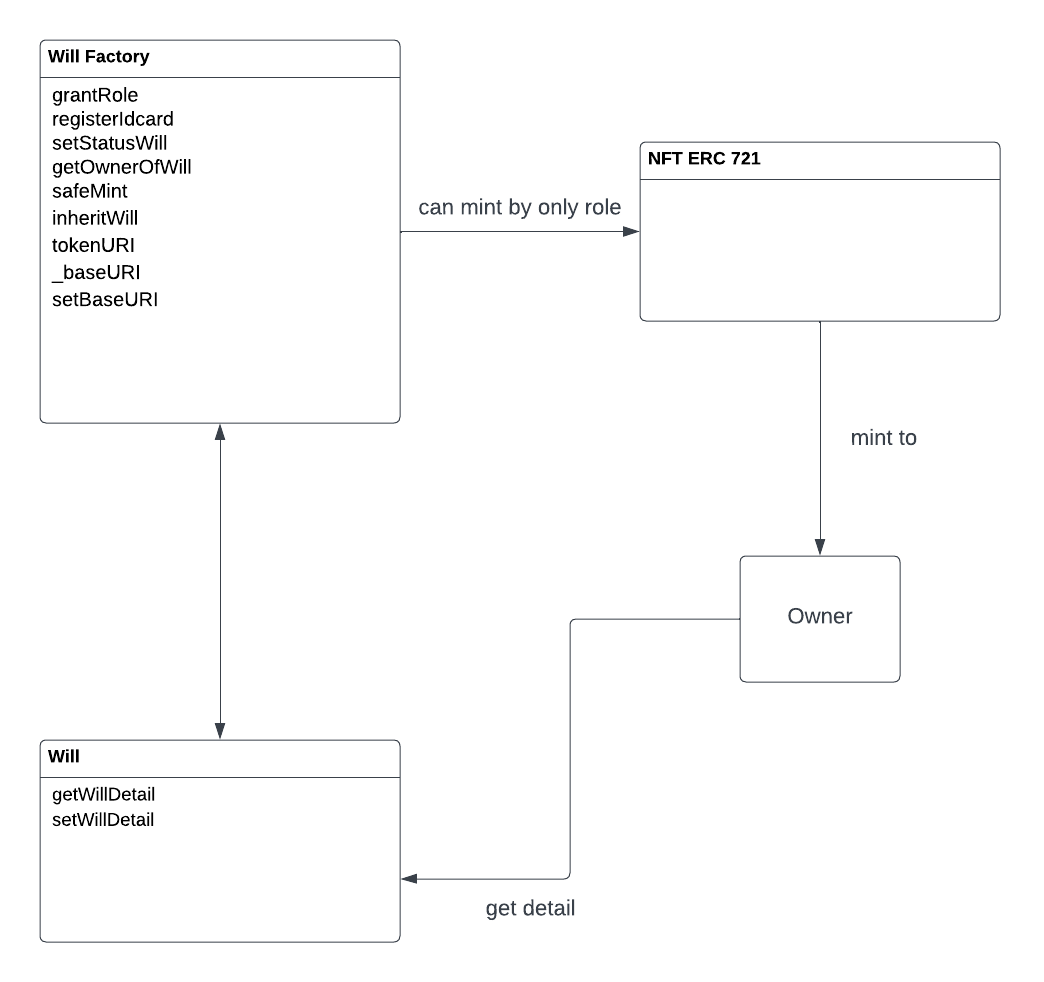
\includegraphics[scale=0.3]{smartContractDiagram}
		\caption{แสดงการ interaction ของ Smart Contract ของระบบ Will Chain}
	\end{figure}
	\FloatBarrier
\tab จากรูปแสดงการทำงานของตัว Smart Contract ของระบบ จะแบ่งเป็น 2 contract ที่ทำหน้าที่ต่างกันโดย will factory จะทำหน้าที่เก็บข้อมูลของทุกพินัยกรรมและรวมถึงการจัดการพินัยกรรมของระบบทั้งหมดโดย will factory สามารถทำการสร้างพินัยกรรมที่เป็น NFT ที่ใช้ ethereum standards ERC 721 และทำการ mint เก็บไว้ที่ตัวเจ้าของพินัยกรรมและเมื่อเกิดเหตุการณ์เสียชีวิตที่ได้รับจากระบบจะมีการ setStatusWill ให้เปลี่ยนเป็น active เพื่อที่จะทำการส่งต่อไปหาผู้รับพินัยกรรม ส่วน contract ต่อมาคือ will เป็น contract ที่ทำหน้าที่เกี่ยวกับจัดการมรดกของแต่ละพินัยกรรม โดยสามารถจัดการได้โดยเจ้าของพินัยกรรมว่าภายในพินัยกรรมของตัวเอง
\clearpage
\subsection{System Architecture Diagram}
	\begin{figure}[!thb]
		\centering
		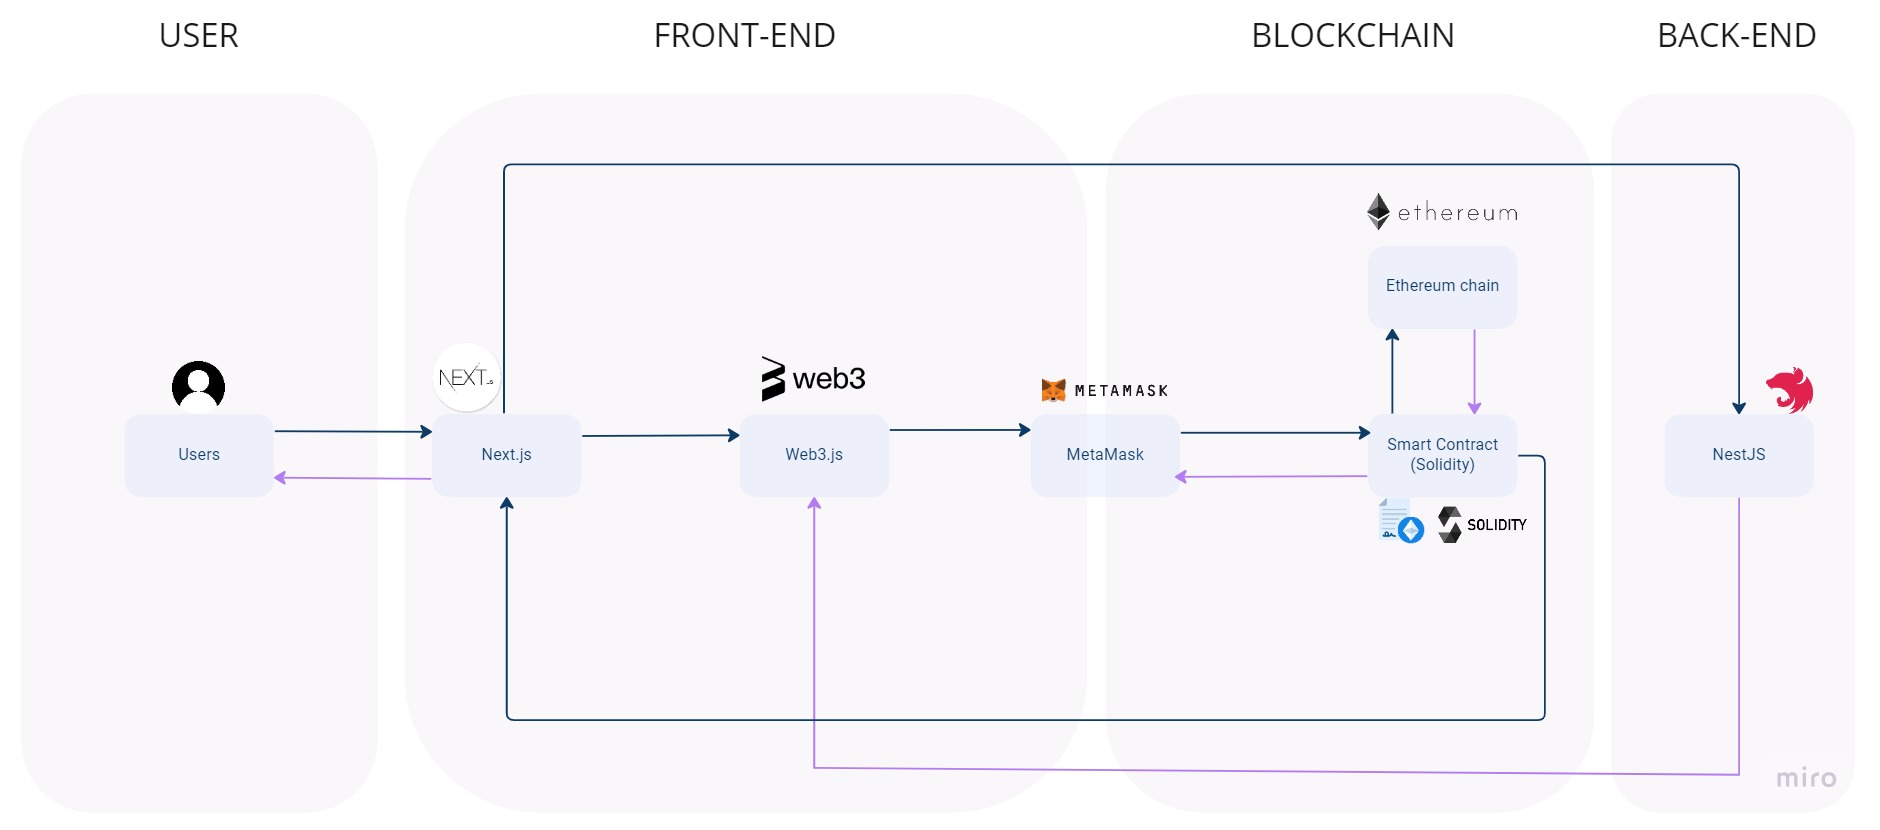
\includegraphics[scale=0.2]{systemArch}
		\caption{แสดงภาพออกแบบสถาปัตยกรรมของระบบ Will Chain}
	\end{figure}
	\FloatBarrier
ระบบของ Will Chain มีส่วนติดต่อกับระบบอื่น ๆ แยกตามประเภทดังนี้ \\
\textbf{Actor ของระบบ}
	\begin{itemize}
		\item User เป็นบุคคลที่ต้องการทำพินัยกรรมของ Will Chain
	\end{itemize}
\textbf{Front-end ของระบบ}
	\begin{itemize}
		\item Next.js จะทำหน้าที่แสดงผล UI ของเว็ปไซต์ Will Chain ในการทำพินัยกรรมต่าง ๆ 
		\item Web3.js จะทำหน้าที่ interact กับ method ต่าง ๆ ใน smart contract
		\item MetaMask จะทำหน้าที่เป็นตัว wallet สำหรับเก็บทรัพย์สินของเราและยังทำหน้าที่เป็นตัว login สำหรับใช้งานในระบบ
	\end{itemize}
\textbf{Blockchain ของระบบ}
	\begin{itemize}
		\item Smart contract จะทำหน้าที่คอยจัดการ transaction ภายใน Ethereum chain
		\item Deploy จะทำหน้าที่ deploy smart contract ขึ้นไปที่ ethereum chain
		\item Ethereum chain จะทำหน้าที่เก็บข้อมูล transaction และการทำพินัยกรรมต่าง ๆ ของระบบ
		\item Pinata จะทำหน้าที่เป็น gateway ในการใช้งาน storage ของระบบพินัยกรรม
	\end{itemize}
\textbf{Storage ของระบบ}
	\begin{itemize}
		\item IPFS จะทำหน้าที่เป็น storage ของระบบพินัยกรรม
	\end{itemize}
\clearpage
\subsection{Sequence Diagram}
	\begin{enumerate}[label=\thesubsection.\arabic*,leftmargin=0pt,itemindent=1.25cm]
	\item Connect MetaMask
		\begin{table}[h]
		\centering
		\caption{ตารางแสดงรายละเอียดของ Connect MetaMask Sequence Diagram}
		\begin{tabularx}{\textwidth}{|l|X|X|} 
			\hline
			Sequence Name: & Connect MetaMask                                                 \\ 
			\hline
			Actors:        & User                                                             \\ 
			\hline
			Pre-Condition: & User จะต้องทำการ Connect MetaMask เพื่อเป็นการ login ใช้งานระบบ  \\
			\hline
		\end{tabularx}
		\end{table}
		\begin{figure}[!thb]
			\centering
			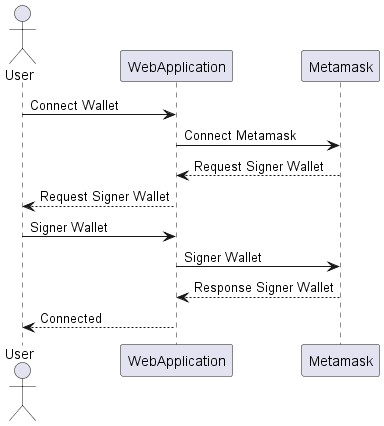
\includegraphics[scale=0.6]{connectMetamaskSeq}
			\caption{แสดง Connect MetaMask Sequence Diagram}
		\end{figure}
		\FloatBarrier
	\tab จากรูป จะเห็นได้ว่าเมื่อผู้ใช้งานทํางาน Connect MetaMask แล้วทาง Web Application จะไปเรียกใช้ MetaMask ที่ทําการติดตั้งไว้ใน Web browser ที่ทําการใช้งานอยู่ว่าขอทำการขอ Signer Wallet เพื่อทําการเชื่อมต่อ Web Application ซึ่งหลังจากทําการ Signer Walet จาก User แล้วตัว Metamask จะทำการ Connected กับ Web Application
\clearpage
	\item Create Will
		\begin{table}[h]
		\centering
		\caption{ตารางแสดงรายละเอียดของ Create Will Sequence Diagram}
		\begin{tabularx}{\textwidth}{|l|X|X|} 
			\hline
			Sequence Name: & Create Will                                                    \\ 
			\hline
			Actors:        & User                                                           \\ 
			\hline
			Pre-Condition  & User จะทำการ Create Will ที่เป็นการเขียนพินัยกรรมผ่านเว็ปไซต์  \\
			\hline
		\end{tabularx}
		\end{table}
		\begin{figure}[!thb]
			\centering
			\includegraphics[scale=0.45]{createWillseq}
			\caption{แสดง Create Will Sequence Diagram}
		\end{figure}
		\FloatBarrier
	\tab จากรูป ผู้ใช้เลือกใช้งาน Create Will จะแสดงหน้าจะแสดงฟอร์มสำหรับการทำพินัยกรรมผ่านระบบ จะทำการ Mint Will Token ไปที่ Metamask หลังจาก Mint NFT เสร็จสิ้นก็ทำการสร้าง Will Contract ที่จะทำหน้าจัดการสินทรัพย์หรือรายละเอียดพินัยกรรมต่าง ๆ ภายในพินัยกรรม หลังจากนั้นจะทำการแสดงผล Token id และ พินัยกรรม ที่ User มีอยู่ 
\clearpage
\item View Will
	\begin{table}[h]
	\centering
	\caption{ตารางแสดงรายละเอียดของ View Will Sequence Diagram}
\begin{tabularx}{\textwidth}{|l|X|X|} 
		\hline
		Sequence Name: & View Will                                  \\ 
		\hline
		Actors:        & User                                       \\ 
		\hline
		Pre-Condition  & User ต้องการดูรายละเอียดพินัยกรรมที่เขียน  \\
		\hline
	\end{tabularx}
	\end{table}
		\begin{figure}[!thb]
			\centering
			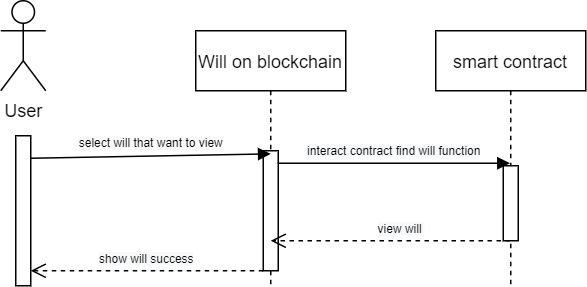
\includegraphics[scale=0.5]{viewWillseq}
			\caption{แสดง View Will Sequence Diagram}
		\end{figure}
		\FloatBarrier
	\tab จากรูป ผู้ใช้ทำการเลือกพินัยกรรมที่ต้องการจะแสดงโดยจะทำการเรียกใช้ฟังก์ชั่นเพื่อดูรายละเอียดใน Will Contract หลังจากนั้น Frontend จะเรียกใช้ฟังก์ชันแสดงสินทรัพย์ดิจิตอล และ เรียกใช้ฟังก์ชันแสดงสินทรัพย์จริง หลังจากนั้นจะทำการแสดงผลของรายละเอียดพินัยกรรม
\item Upload Will
		\begin{table}[h]
		\centering
		\caption{ตารางแสดงรายละเอียดของ Upload Pdf Will Sequence Diagram}
		\begin{tabularx}{\textwidth}{|l|X|X|} 
			\hline
			Sequence Name: & Upload Will                                             \\ 
			\hline
			Actors:        & User                                                        \\ 
			\hline
			Pre-Condition  & User จะทำการ Upload ที่เป็นการเขียนพินัยกรรมด้วยลายมือ  \\
			\hline
		\end{tabularx}
		\end{table}
		\begin{figure}[!thb]
			\centering
			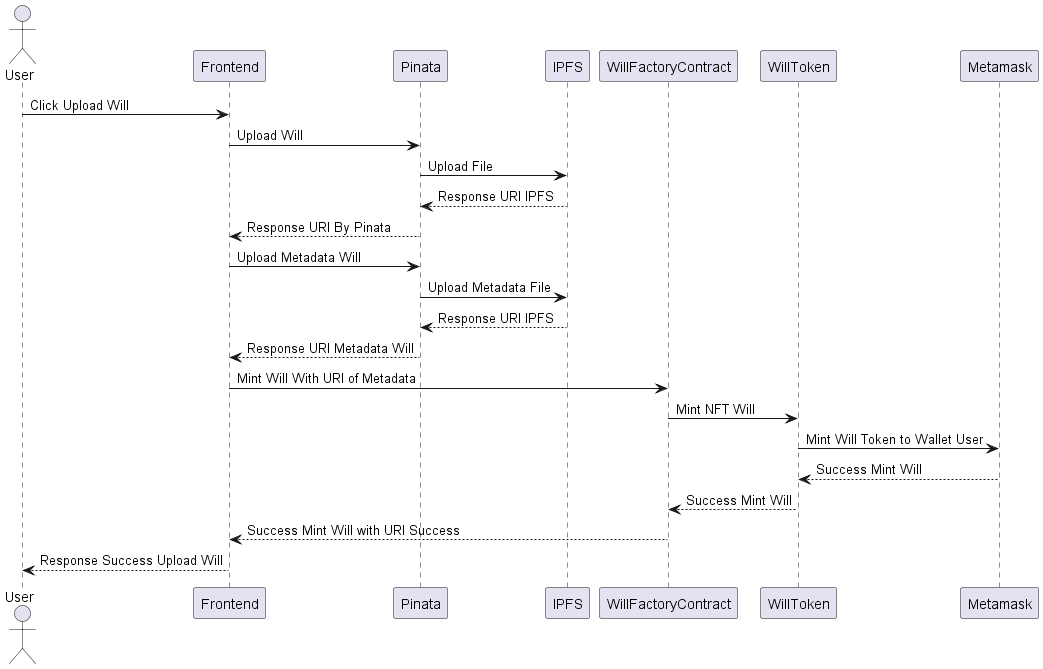
\includegraphics[scale=0.4]{uploadWillseq}
			\caption{แสดง Upload Will Sequence Diagram}
		\end{figure}
		\FloatBarrier
	\tab จากรูป ผู้ใช้เลือกใช้งาน Upload พินัยกรรมที่เขียนด้วยมือระบบจะแสดงฟอร์มที่ใช้สำหรับการ Upload พินัยกรรมไปที่ Pinata และ Pinata ทำหน้าที่ Upload File ไปที่ IPFS หลังจากนั้น IPFS จะส่ง URI ไปที่ Pinata จะทำการส่งต่อไปที่ Frontend หลังจากนั้น Upload Metadata Will หลังจากนั้น Pinata จะ Upload Metada Will ไปที่ IPFS หลังจากนั้น IPFS จะส่ง URI ไปที่ Pinata หลังจากนั้นส่งไป Frontend เพื่อทำการ mint Will Token ออกมาโดยสั่ง mint ไปที่ Will Factory Contract เพื่อทำการจัดการ Mint Will Token หลังจากนั้นจะทำการ Mint Will Token ไปที่ Metamask wallet ของ User หลังจากนั้น Frontend จะแสดงผลอัพโหลดพินัยกรรมเสร็จสิ้น
	\item Delete Will
	\begin{table}[h]
		\centering
		\caption{ตารางแสดงรายละเอียดของ Delete Will Sequence Diagram}
		\begin{tabularx}{\textwidth}{|l|X|X|} 
			\hline
			Sequence Name: & Delete Will                           \\ 
			\hline
			Actors:        & User                                  \\ 
			\hline
			Pre-Condition  & User ต้องการที่จะลบพินัยกรรมที่เขียน  \\
			\hline
		\end{tabularx}
	\end{table}
		\begin{figure}[!thb]
			\centering
			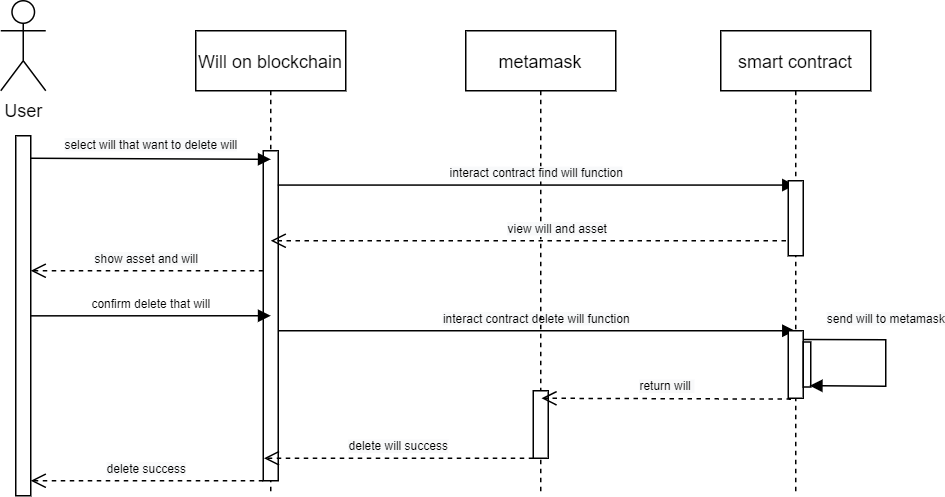
\includegraphics[scale=0.5]{deleteWillseq}
			\caption{แสดง Delete Will Sequence Diagram}
		\end{figure}
		\FloatBarrier
	\tab จากรูป ผู้ใช้ต้องการทำการลบ พินัยกรรมที่มีอยู่ในระบบ โดยระบบจะทำการ Burn Will Token ของเหรียญที่แทนพินัยกรรมนั้นหลังจากนั้นทำการลบพินัยกรรมที่ทำการเลือดไว้ใน WillFactoryContract หลังจากลบเสร็จสิ้นจะแสดงผลหน้าจอว่าลบพินัยกรรมสำเร็จ 
\clearpage
\item View Beneficiary
	\begin{table}[h]
	\centering
	\caption{ตารางแสดงรายละเอียดของ View Beneficiary Sequence Diagram}
	\begin{tabularx}{\textwidth}{|l|X|X|} 
		\hline
		Sequence Name: & View Beneficiary                                    \\ 
		\hline
		Actors:        & User                                                  \\ 
		\hline
		Pre-Condition  & User ต้องการดูผู้รับพินัยกรรมที่อยู่ระบบ \\
		\hline
		\end{tabularx}
	\end{table}
		\begin{figure}[!thb]
			\centering
			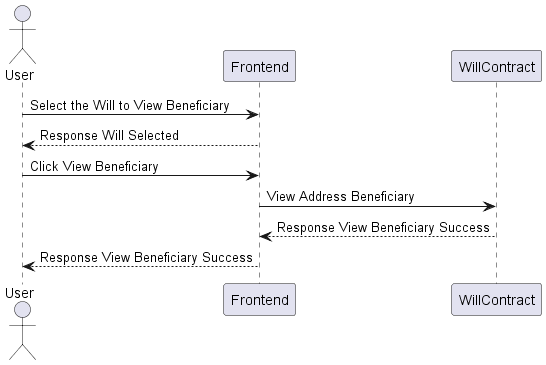
\includegraphics[scale=0.6]{viewBeneficiaryseq}
			\caption{แสดง View Beneficiary Sequence Diagram}
		\end{figure}
		\FloatBarrier
	\tab จากรูป ผู้ใช้ต้องเลือกพินัยกรรมที่ต้องการดูผู้รับพินัยกรรม และจะแสดงรายละเอียดพินัยกรรมหลังจากนั้นคลิกดูพินัยกรรมและ Frontend จะเรียกฟังก์ชั่นแสดงผู้รับพินัยกรรมจาก Will Contract หลังจากได้รับข้อมูลจาก Will Contract ตัว Frontend จะทำการแสดงผล Address ของ Beneficiary 
\item Set Beneficiary
	\begin{table}[h]
	\centering
	\caption{ตารางแสดงรายละเอียดของ Set Beneficiary Sequence Diagram}
	\begin{tabularx}{\textwidth}{|l|X|X|} 
		\hline
		Sequence Name: & Set Beneficiary                                  \\ 
		\hline
		Actors:        & User                                                  \\ 
		\hline
		Pre-Condition  & User ต้องการเลือกผู้รับพินัยกรรมที่อยู่ระบบ \\
		\hline
		\end{tabularx}
	\end{table}
		\begin{figure}[!thb]
			\centering
			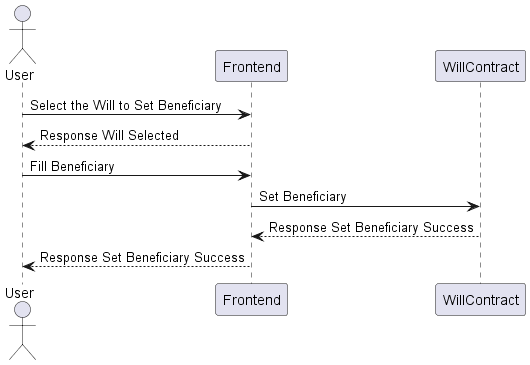
\includegraphics[scale=0.6]{setBeneficiaryseq}
			\caption{แสดง Set Beneficiary Sequence Diagram}
		\end{figure}
		\FloatBarrier
	\tab จากรูป ผู้ใช้ต้องเลือกพินัยกรรมที่ต้องการดูผู้รับพินัยกรรม และจะแสดงรายละเอียดพินัยกรรมหลังจากนั้นคลิกช่อง Beneficiary และใส่เลข Address ของ Beneficiary หลังจากนั้น Frontend จะทำการเรียกฟังก์ชัน setBeneficiary เพื่อทำการเพิ่มผู้รับพินัยกรรมใน will contract และหลังจากเพิ่มพินัยกรรมเสร็จสิ้นก็ทำการแสดงผลว่าเพิ่มผู้รับพินัยกรรมเสร็จสิ้น
	\item View Assets
	\begin{table}[h]
	\centering
	\caption{ตารางแสดงรายละเอียดของ View Assets Sequence Diagram}
	\begin{tabularx}{\textwidth}{|l|X|X|} 
		\hline
		Sequence Name: & View Assets                                \\ 
		\hline
		Actors:        & User                                                  \\ 
		\hline
		Pre-Condition  & User ต้องการดูสินทรัพย์ที่เชื่อมต่อ Smart
		  Contract  \\
		\hline
		\end{tabularx}
	\end{table}
		\begin{figure}[!thb]
			\centering
			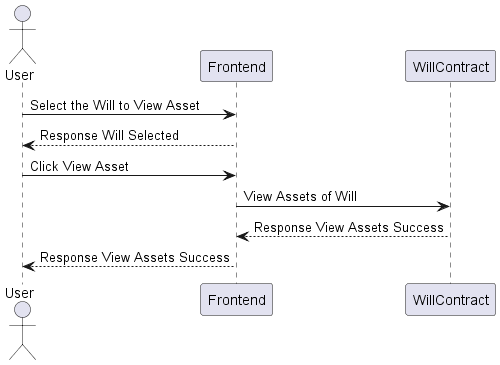
\includegraphics[scale=0.6]{viewAssetseq}
			\caption{แสดง View Assets Sequence Diagram}
		\end{figure}
		\FloatBarrier
	\tab จากรูป ผู้ใช้ต้องเลือกพินัยกรรมที่ต้องการดูผู้รับพินัยกรรม และจะแสดงรายละเอียดพินัยกรรมหลังจากนั้นคลิกดูสินทรัพย์และ Frontend จะเรียกฟังก์ชั่นแสดงสินทรัพย์จาก Will Contract หลังจากได้รับข้อมูลจาก Will Contract ตัว Frontend จะทำการแสดงผลสินทรัพย์เสร็จสิ้น
\item Deposit Digital Assets
	\begin{table}[h]
	\centering
	\caption{ตารางแสดงรายละเอียดของ Deposit Digital Assets Sequence Diagram}
	\begin{tabularx}{\textwidth}{|l|X|X|} 
		\hline
		Sequence Name: & Deposit Digital Assets                             \\ 
		\hline
		Actors:        & User                                                  \\ 
		\hline
		Pre-Condition  & User ต้องการเพิ่มสินทรัพย์ดิจิทัลที่เชื่อมต่อ Smart
		  Contract  \\
		\hline
		\end{tabularx}
	\end{table}
		\begin{figure}[!thb]
			\centering
			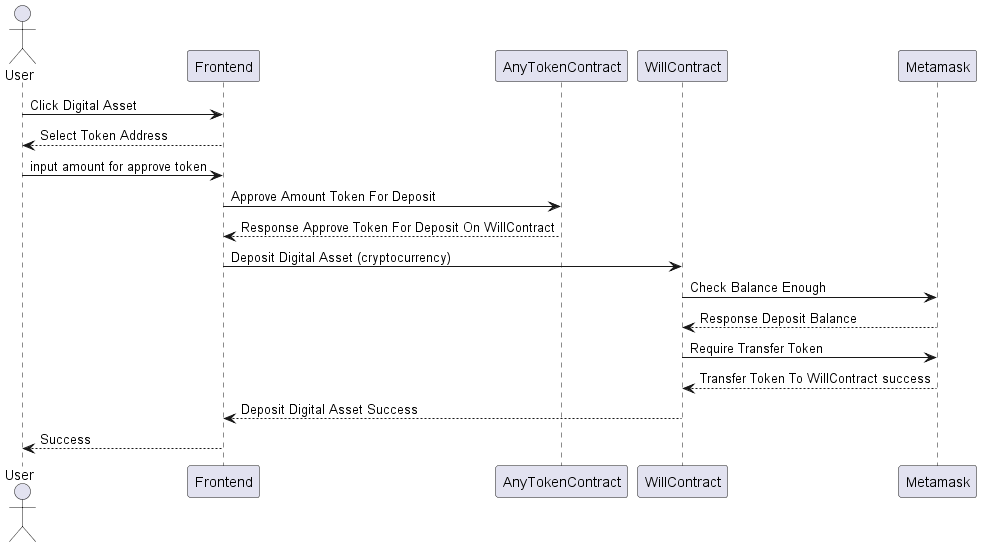
\includegraphics[scale=0.4]{depositDigitalseq}
			\caption{แสดง Deposit Digital Assets Sequence Diagram}
		\end{figure}
		\FloatBarrier
	\tab จากรูป ผู้ใช้ต้องการเพิ่มสินทรัพย์ดิจิทัลจะทำการคลิกเพื่อสินทรัพย์ดิจิทัลและทำการเลือกเหรียญที่ต้องการฝากไว้ในพินัยกรรมและ Frontend  จะทำการ Approve จำนวนของตัว Token นั้นที่จะทำการ Deposit เข้า Smart Contract หลังจากนั้น Frontend จะทำการ Deposit Digital Assets ไปที่ Will Contract และจะทำการเช็คยอดเงินคงเหลือใน Metamask ว่าเพียงพอต่อการฝากและหลังจากนั้นจะใช้ฟังก์ชั่นใน Will Contract Transfer เหรียญที่อยู่ใน Metamask ไปที่ Will Contract และหลังจากนั้น Frontend จะแสดงผลการเพิ่มสินทรัพย์ดิจิทัลเสร็จสิ้น
\item Deposit Real Assets
	\begin{table}[h]
	\centering
	\caption{ตารางแสดงรายละเอียดของ Deposit Real Assets Sequence Diagram}
	\begin{tabularx}{\textwidth}{|l|X|X|} 
		\hline
		Sequence Name: & Deposit Real Assets                          \\ 
		\hline
		Actors:        & User                                                  \\ 
		\hline
		Pre-Condition  & User ต้องการเพิ่มสินทรัพย์จริงที่เชื่อมต่อ Smart
		  Contract  \\
		\hline
		\end{tabularx}
	\end{table}
		\begin{figure}[!thb]
			\centering
			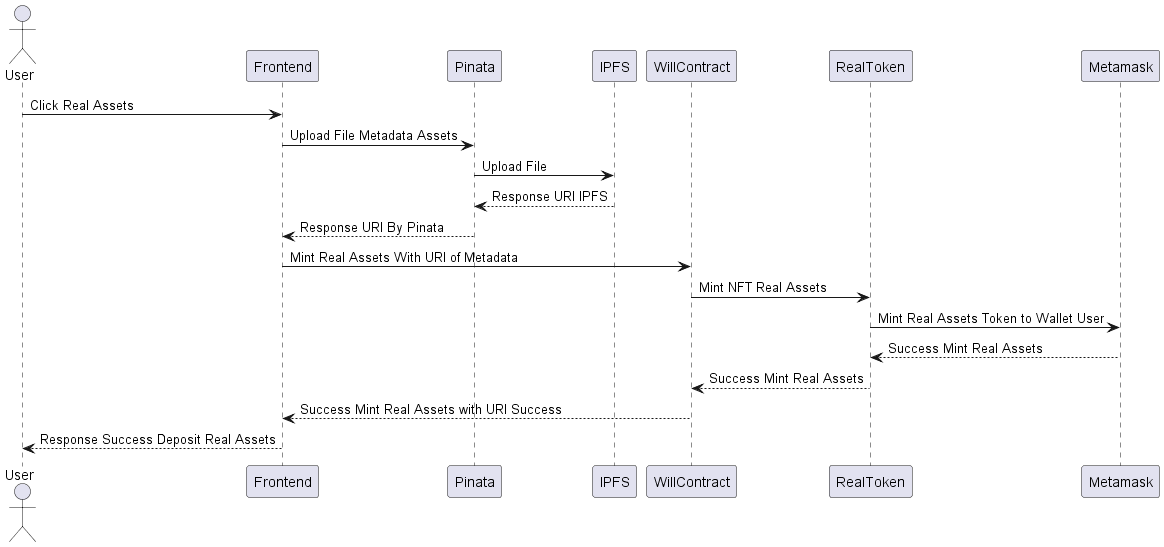
\includegraphics[scale=0.35]{depositRealseq}
			\caption{แสดง Deposit Real Assets Sequence Diagram}
		\end{figure}
		\FloatBarrier
	\tab จากรูป ผู้ใช้ต้องการเพิ่มสินทรัพย์จริงจะทำการคลิกเพื่อสินทรัพย์ดิจิทัล Frontend จะทำการอัพโหลด Metadata ของ Assets ไปที่ Pinata และ Pinata ทำหน้าที่ Upload File ไปที่ IPFS หลังจากนั้น IPFS จะส่ง URI ไปที่ Pinata จะทำการส่งต่อไปที่ Frontend หลังจากนั้น Frontend ทำการ mint Real Token ออกมาโดยสั่ง mint ไปที่ Will Contract เพื่อทำการจัดการ Mint Real Token หลังจากนั้นจะทำการ Mint Real Token ไปที่ Metamask wallet ของ User หลังจากนั้น Frontend จะแสดงผลเพิ่มสินทรัพย์จริงเสร็จสิ้น
\item Active Will
	\begin{table}[h]
\centering
\caption{ตารางแสดงรายละเอียดของ Active Will Sequence Diagram}
\begin{tabularx}{\textwidth}{|l|X|X|} 
\hline
Sequence Name: & Active Will                                          \\ 
\hline
Actors:        & Controller                                           \\ 
\hline
Pre-Condition  & ผู้กำกับพินัยกรรมต้องการเริ่มการสืบทอดพินัยกรรม  \\
\hline
\end{tabularx}
\end{table}
		\begin{figure}[!thb]
			\centering
			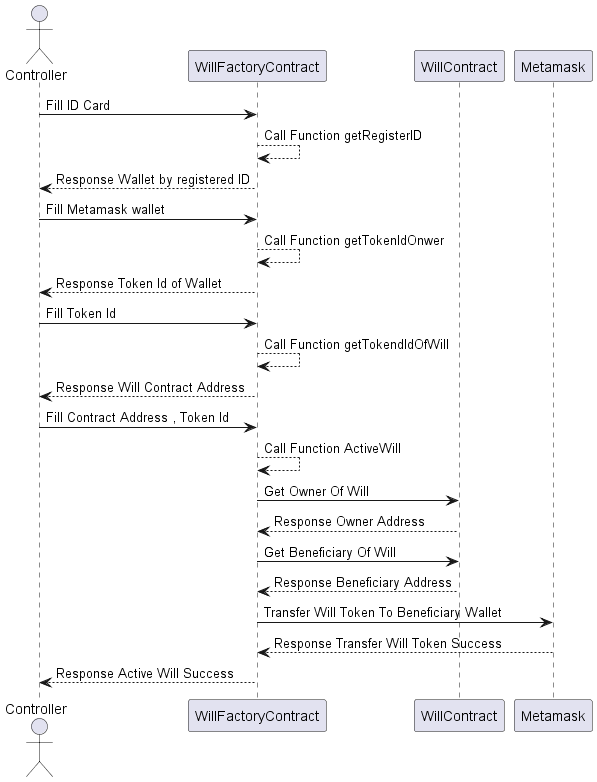
\includegraphics[scale=0.45]{activeWillseq}
			\caption{แสดง Active Will Sequence Diagram}
		\end{figure}
		\FloatBarrier
	\tab จากรูป ผู้ควมคุมจะทำการกรอก ID Card ไว้และเพื่อนำเลข Wallet Address ที่ทำการ register กับระบบไว้หลังจากนั้นจะกรอกเลขกระเป๋าเพื่อนำเลข Token id ที่เจ้าของพินัยกรรมถืออยู่มีอะไรบ้างหลังจากนั้น จะทำการกรอก token id เพื่อนำเลข Will Factory Contract address ไปทำการกรอกฟังก์ชั่น ActiveWill เพื่อทำการให้พินัยกรรมนี้สามารถทำงานได้ โดยจะใช้กระเป๋าของเจ้าของพินัยกรรมและกระเป๋าของผู้รับพินัยกรรม และทำการส่ง Will Token ไปที่ กระเป๋าของผู้รับพินัยกรรม
	\item Claim Assets
	\begin{table}[h]
\centering
\caption{ตารางแสดงรายละเอียดของ Claim Assets Sequence Diagram}
\begin{tabularx}{\textwidth}{|l|X|X|} 
\hline
Sequence Name: & Claim Asset                                             \\ 
\hline
Actors:        & Beneficiary                                            \\ 
\hline
Pre-Condition  & ทายาทจะทำการรับสินทรัพย์ที่ได้รับจากการเขียนพินัยกรรม  \\
\hline
\end{tabularx}
\end{table}
		\begin{figure}[!thb]
			\centering
			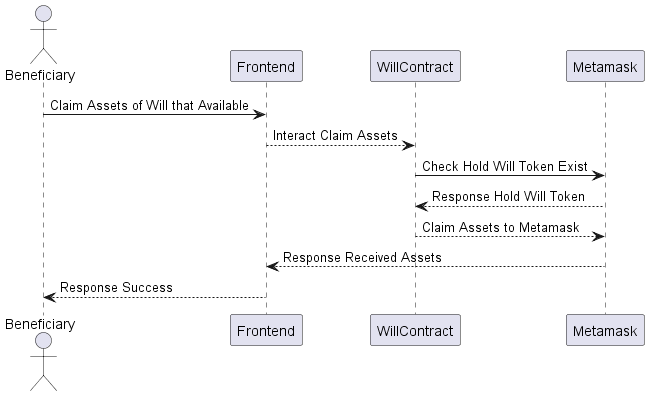
\includegraphics[scale=0.45]{claimAssetseq}
			\caption{แสดง Claim Assets Sequence Diagram}
		\end{figure}
		\FloatBarrier
	\tab จากรูป ทายาทจะรับสินทรัพย์ที่ได้รับจากการเขียนพินัยกรรมโดย Will Contract จะไปเช็ึคใน Metamask ว่า ลูกมี Will Token ที่สามารถ interact กับ Will Contract นี้ไหม หลังจากนั้นจะให้ผู้รับพินัยกรรมรับสินทรัพย์ที่อยู่ใน Will Contract ได้ไปที่ Metamask หลังจากนั้น Frontend จะแสดงผลรับสินทรัพย์เสร็จสิ้น
	\end{enumerate}
\clearpage
\section{ส่วนติดต่อผู้ใช้งาน (User Interface)}
\tab การออกแบบส่วนติดต่อผู้ใช้งาน โดยการออกแบบ Will Chain ได้คำนึงถึงการใช้งานของผู้ใช้งาน 
\subsection{หน้าแรก}
		\begin{figure}[!thb]
			\centering
			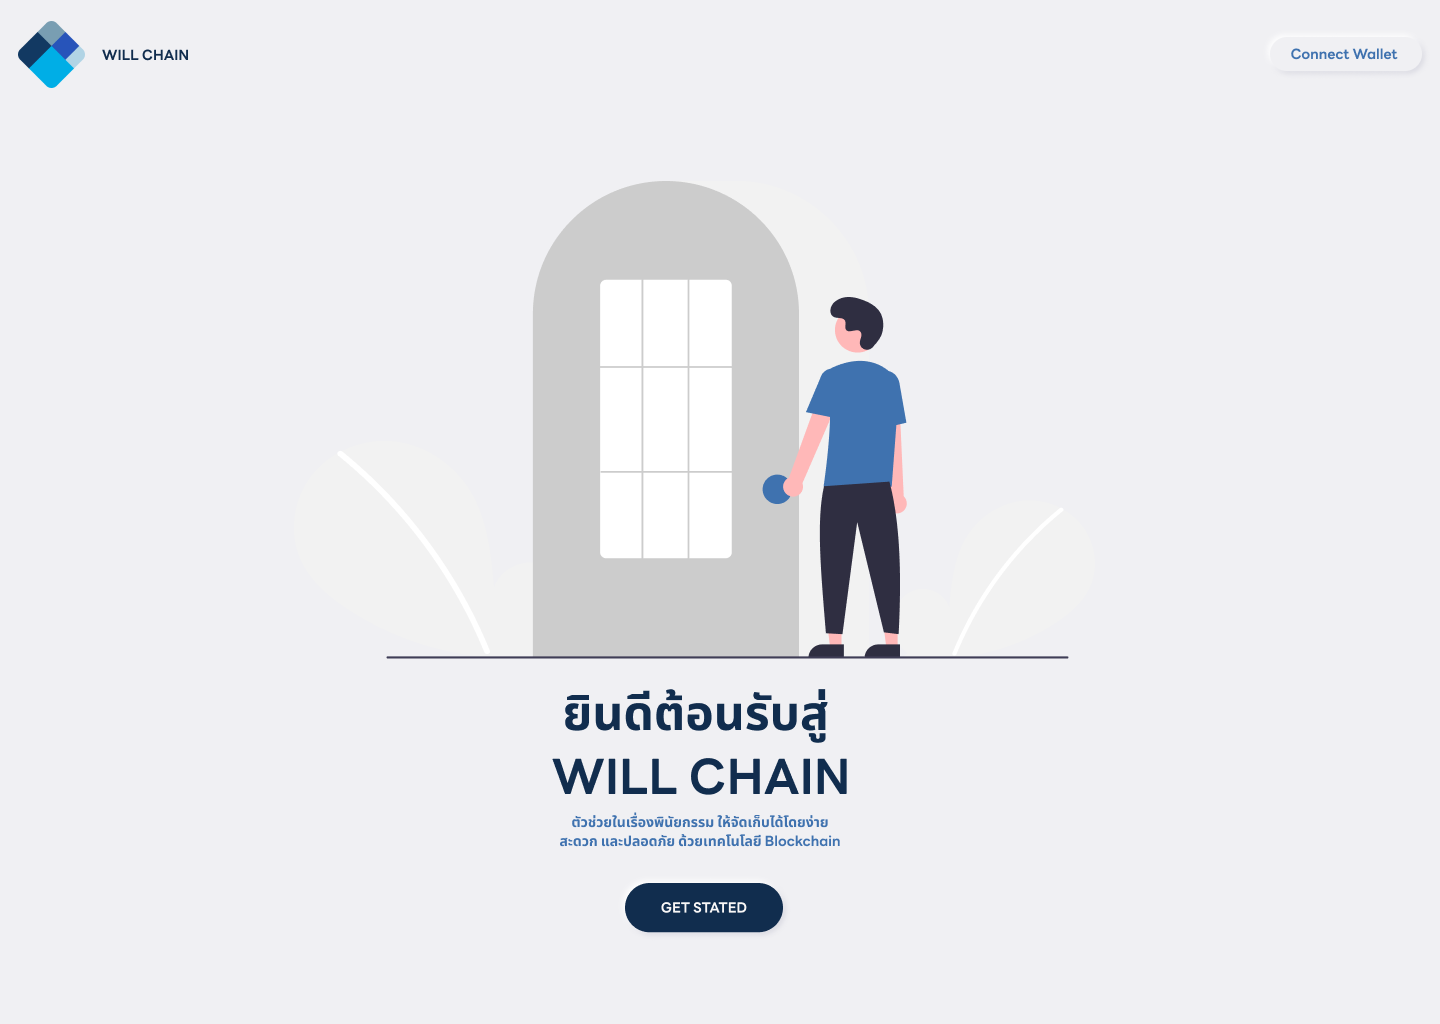
\includegraphics[scale=0.2]{Home}
			\caption{หน้าแรก}
		\end{figure}
		\FloatBarrier
		\tab จากรูปเป็นหน้าแรกของแพลตฟอร์ม Web application Will Chain ที่ยังไม่ได้ทำการเข้าสู่ระบบ โดยจะประกอบไปด้วย Concept ของแพลตฟอร์ม รวมไปถึงการเข้าถึงคู่มือการใช้งาน และยังสามารถที่ปุ่มขวาบนเพื่อเชื่อมต่อกับ MetaMask Wallet
\subsection{หน้าโปรไฟล์}
		\begin{figure}[!thb]
			\centering
			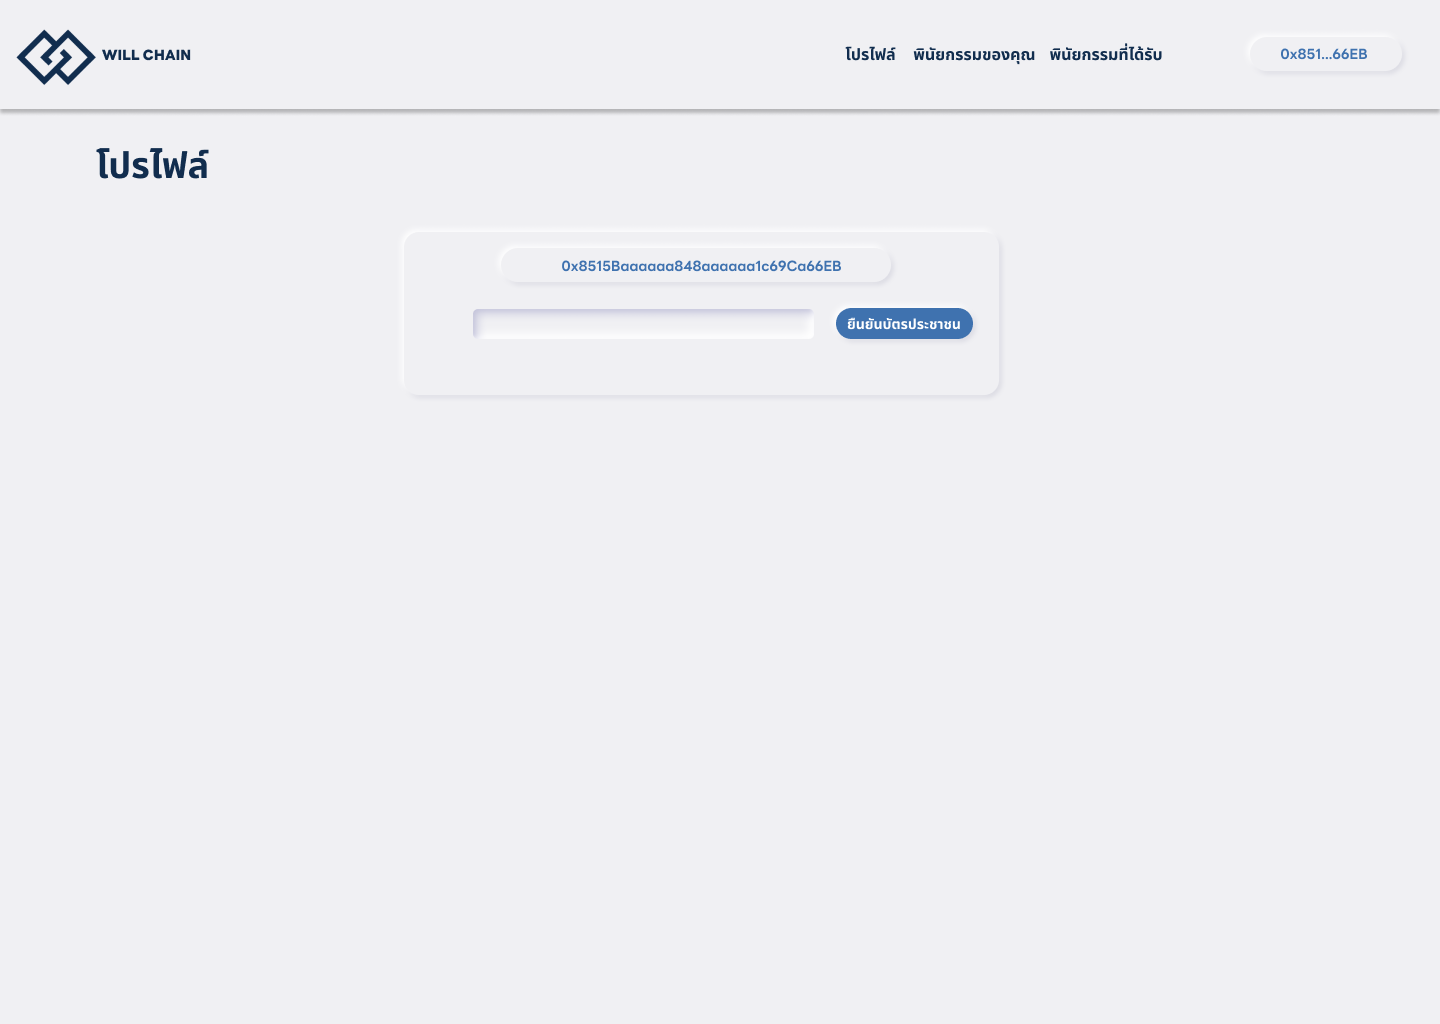
\includegraphics[scale=0.2]{profile}
			\caption{หน้าโปรไฟล์}
		\end{figure}
		\FloatBarrier
		\tab จากรูปเป็นหน้าโปรไฟล์จะต้องทำการ Connect Metamask โดยจะแสดงเลข Public key ทางด้านขวาบน จะเข้ามาสู่หน้าโปรไฟล์ ที่จะมีแสดงเลข Public key ของ MetaMask และมีช่องให้ใส่เลขบัตรประจำตัวประชาชน เพื่อยืนยันสำหรับการสืบทอดพินัยกรรม
\subsection{หน้าโปรไฟล์ยืนยันการลงทะเบียน}
		\begin{figure}[!thb]
			\centering
			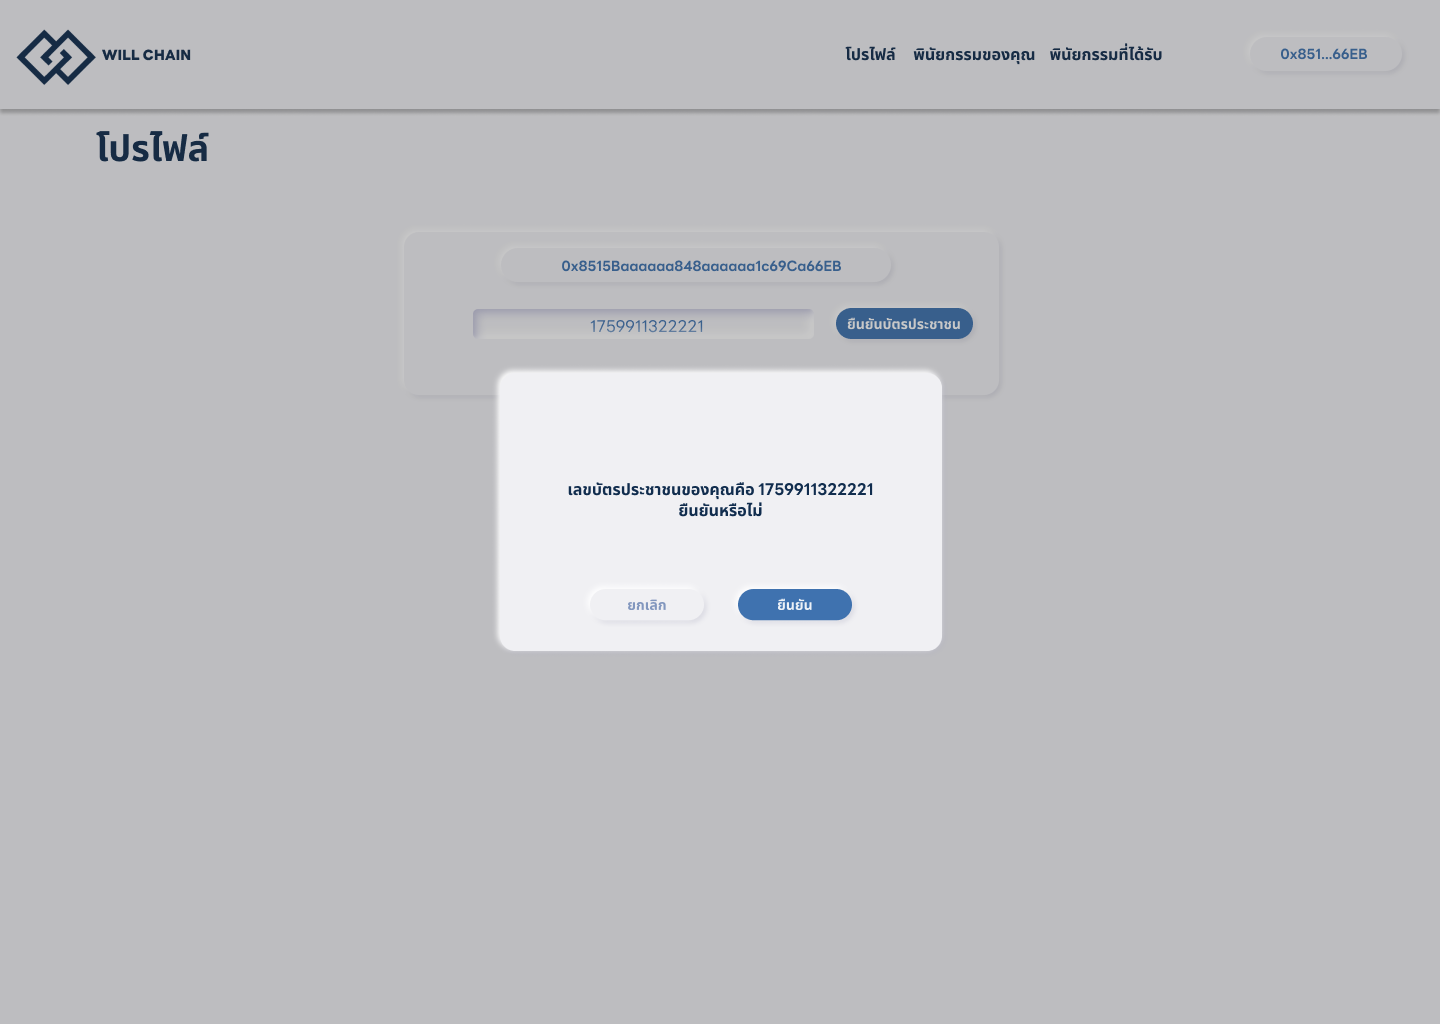
\includegraphics[scale=0.2]{profileConfirm}
			\caption{หน้าโปรไฟล์ ยืนยันการลงทะเบียน}
		\end{figure}
		\FloatBarrier
		\tab จากรูปเป็นหน้าโปรไฟล์หลักจากดปุ่มยืนยันการลงทะเบียนด้วยรหัสเลขบัตรประชาชน
\subsection{หน้าโปรไฟล์ลงทะเบียนสำเร็จ}
		\begin{figure}[!thb]
			\centering
			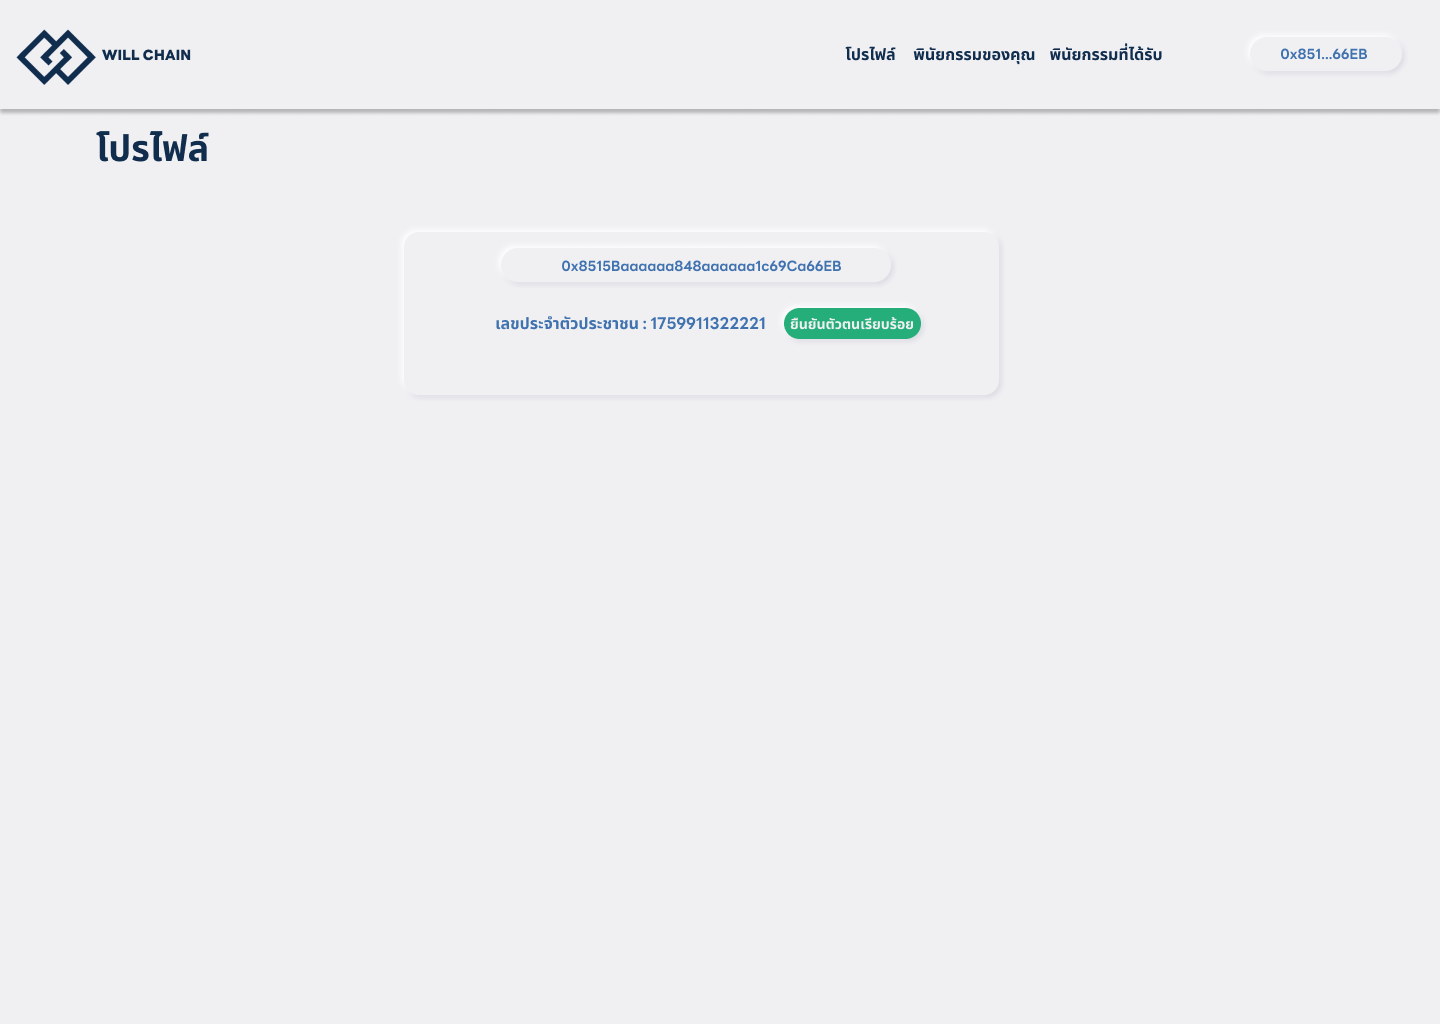
\includegraphics[scale=0.2]{profileSuccess}
			\caption{หน้าโปรไฟล์ ยืนยันการลงทะเบียนสำเร็จ}
		\end{figure}
		\FloatBarrier
		\tab จากรูปเป็นหน้าโปรไฟล์ที่เมื่อทำการกรอกการลงทะเบียนด้วยเลขบัตรประชาชน
\subsection{หน้าพินัยกรรมของคุณ}
		\begin{figure}[!thb]
			\centering
			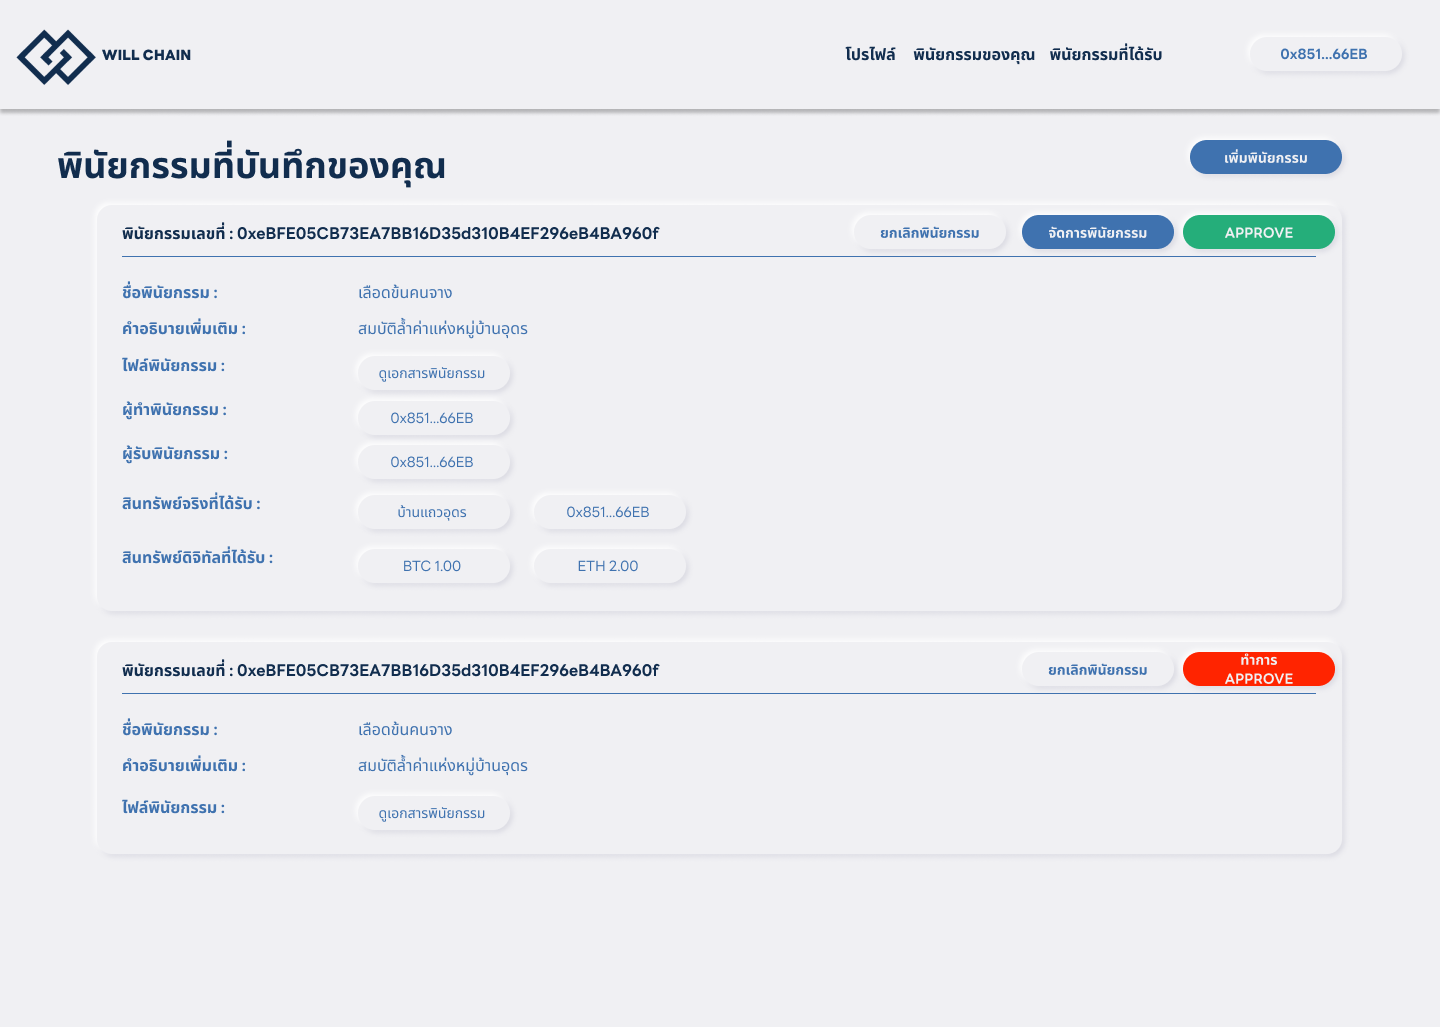
\includegraphics[scale=0.2]{userWill}
			\caption{หน้าพินัยกรรมของคุณ}
		\end{figure}
		\FloatBarrier
		\tab จากรูปเป็นหน้าพินัยกรรมของคุณ จากการกดที่เมนู “พินัยกรรมของคุณ” ด้านบน โดยที่ในหน้านี้จะแสดงพินัยกรรมที่มีอยู่ในระบบของผู้ใช้คนนี้ โดยที่ใน 1 พินัยกรรม จะแสดงเลขฉบับที่ของพินัยกรรม สถานะของพินัยกรรม และสามารถกดปุ่ม “ดูพินัยกรรม” เพื่อดูพินัยกรรมที่เป็นไฟล์ฉบับจริงได้ โดยในตารางด้านล่างนั้นจะแสดงจำนวนผู้รับพินัยกรรมและรายชื่อของคนที่รับพินัยกรรม ต่อมาคือแสดงสินทรัพย์ทั้งหมดที่อยู่ในพินัยกรรมฉบับนี้ และแสดงสินทรัพย์ สุดท้ายคือแสดงสินทรัพย์ดิจิทัลทั้งหมดในพินัยกรรมนั้น และแสดงชนิดของสินทรัพย์ดิจิทัล โดยที่สามารถกดที่ปุ่ม “ดูข้อมูล” เพื่อดูข้อมูลเพิ่มเติม และสามารถกดปุ่ม “ลบพินัยกรรม” เพื่อลบพินัยกรรมนั้นออกจากระบบได้

\subsection{หน้ายกเลิกการทำพินัยกรรมของคุณ}
		\begin{figure}[!thb]
			\centering
			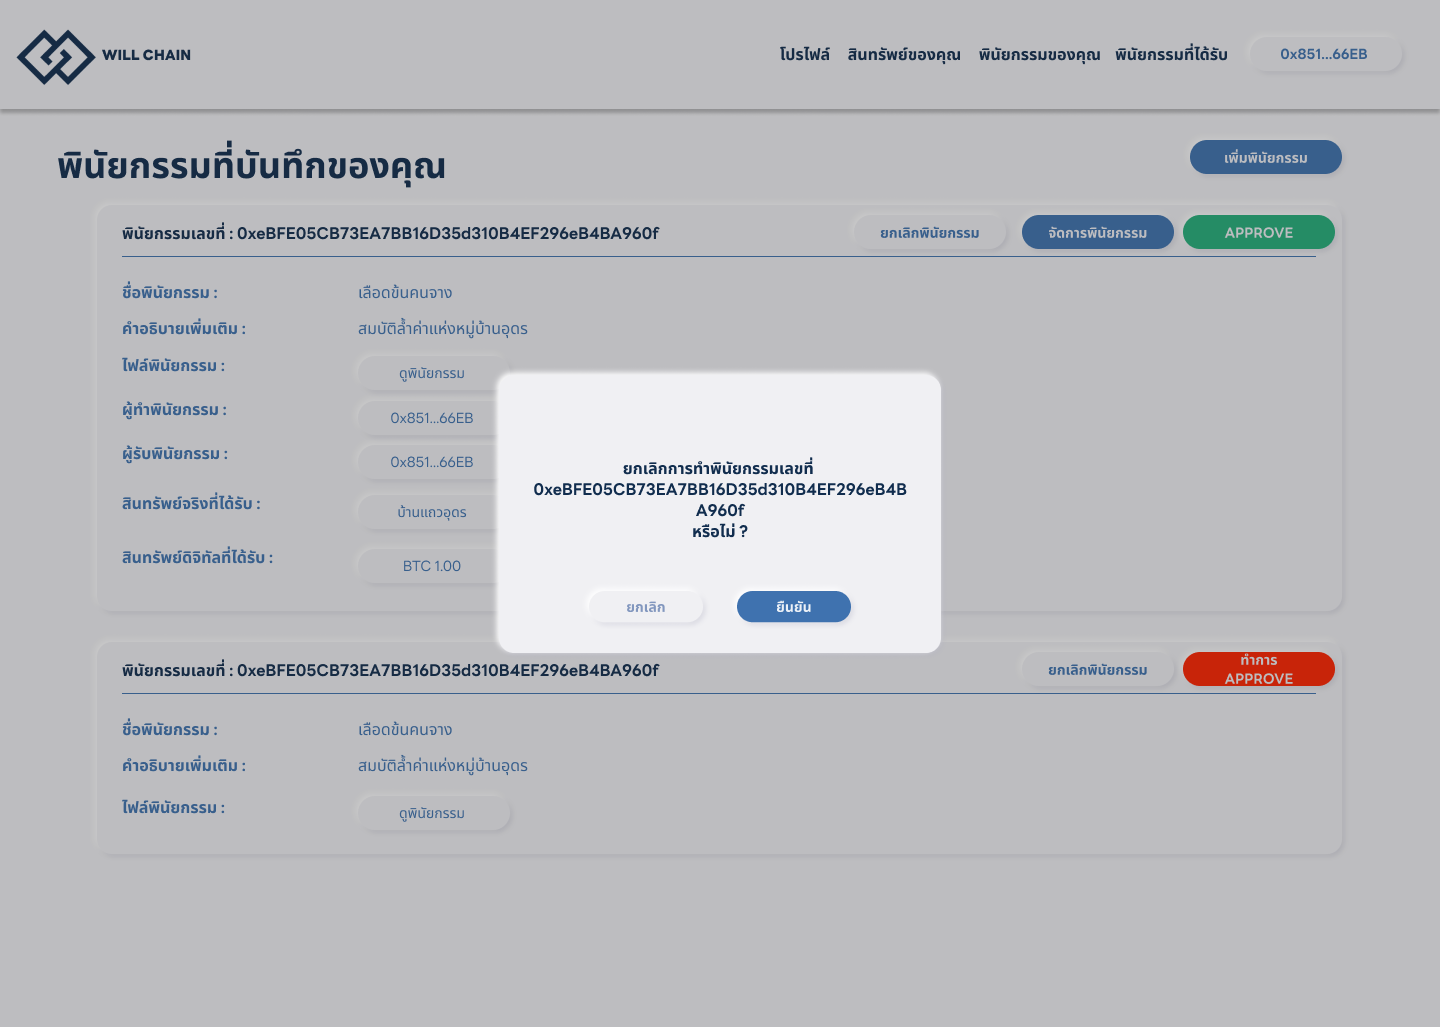
\includegraphics[scale=0.2]{cancelWill}
			\caption{หน้ายกเลิกการทำพินัยกรรมของคุณ}
		\end{figure}
		\FloatBarrier
		\tab จากรูปเป็นจะเป็นหน้ายกเลิกการทำพินัยกรรม จากการที่กดเมนู "ยกเลิกพินัยกรรม" ในหน้าพินัยกรรมของคุณ โดยที่หน้านีจะแสดงยืนยันการลบพินัยกรรมฉบับนั้น
\subsection{หน้า Approve พินัยกรรมของคุณ}
		\begin{figure}[!thb]
			\centering
			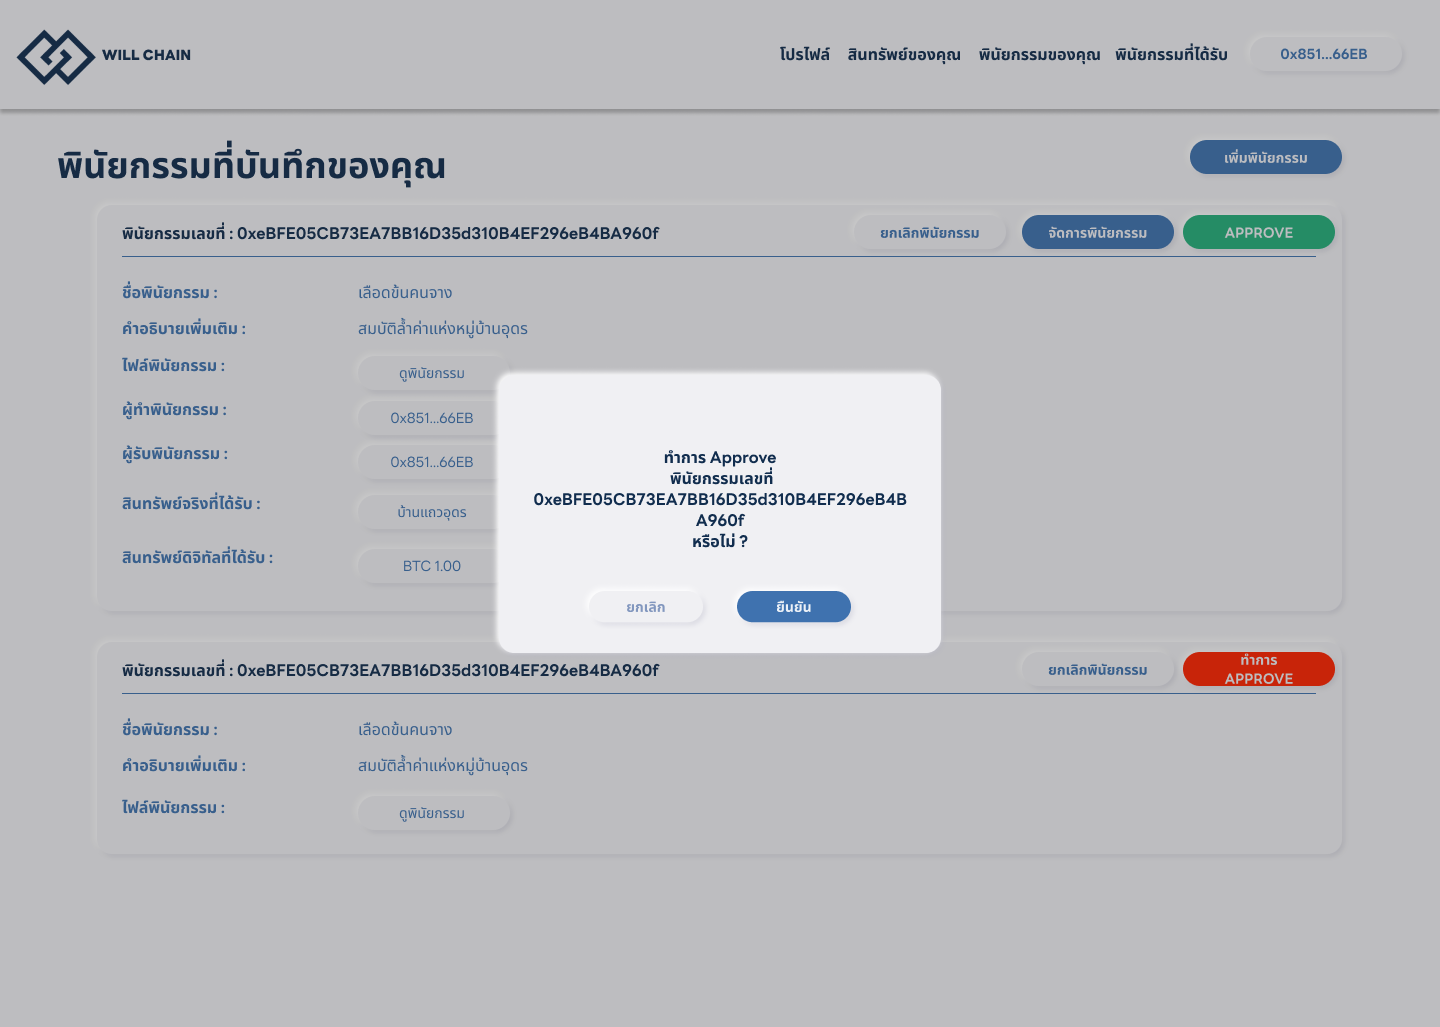
\includegraphics[scale=0.2]{WillApprove}
			\caption{หน้า Approve พินัยกรรมของคุณ}
		\end{figure}
		\FloatBarrier
		\tab จากรูปเป็นจะเป็นหน้า Approve พินัยกรรม จากการที่กดเมนู "ทำการ Approve" ในหน้าพินัยกรรมของคุณ โดยที่หน้านีจะแสดงยืนยันการ Approve ของพินัยกรรมให้ระบบของ Will Chain ดูแลเรื่องพินัยกรรมให้
\subsection{หน้าบันทึกพินัยกรรม}
		\begin{figure}[!thb]
			\centering
			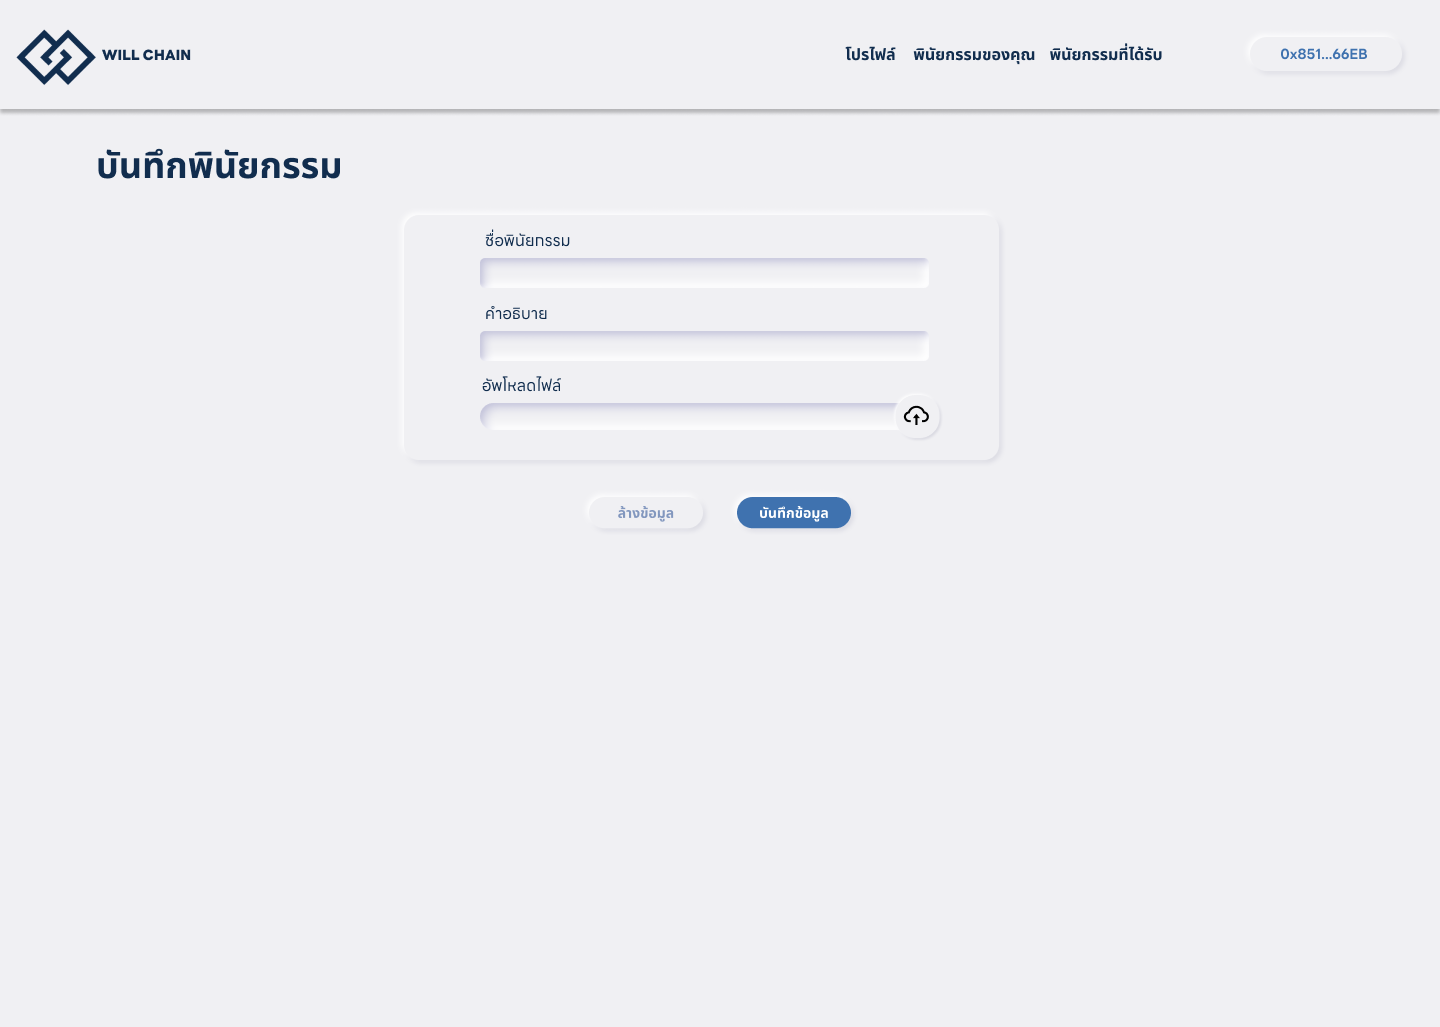
\includegraphics[scale=0.2]{saveWill}
			\caption{หน้าบันทึกพินัยกรรม}
		\end{figure}
		\FloatBarrier
		\tab  จากรูปเป็นหน้าบันทึกพินัยกรรม โดยสามารถบันทึกพินัยกรรมได้ที่หน้านี้ โดยจะเข้าหน้านี้หลังจากกดที่ปุ่ม “เพิ่มพินัยกรรม” ในหน้าพินัยกรรมของคุณ โดยที่จะมีฟอร์มคือพินัยกรรมที่จะให้ใส่ชื่อพินัยกรรม รายละเอียดของพินัยกรรมฉบับนี้และอัพโหลดไฟล์พินัยกรรมฉบับจริง
\subsection{หน้าจัดการสินทรัพย์ภายในพินัยกรรมของคุณ}
		\begin{figure}[!thb]
			\centering
			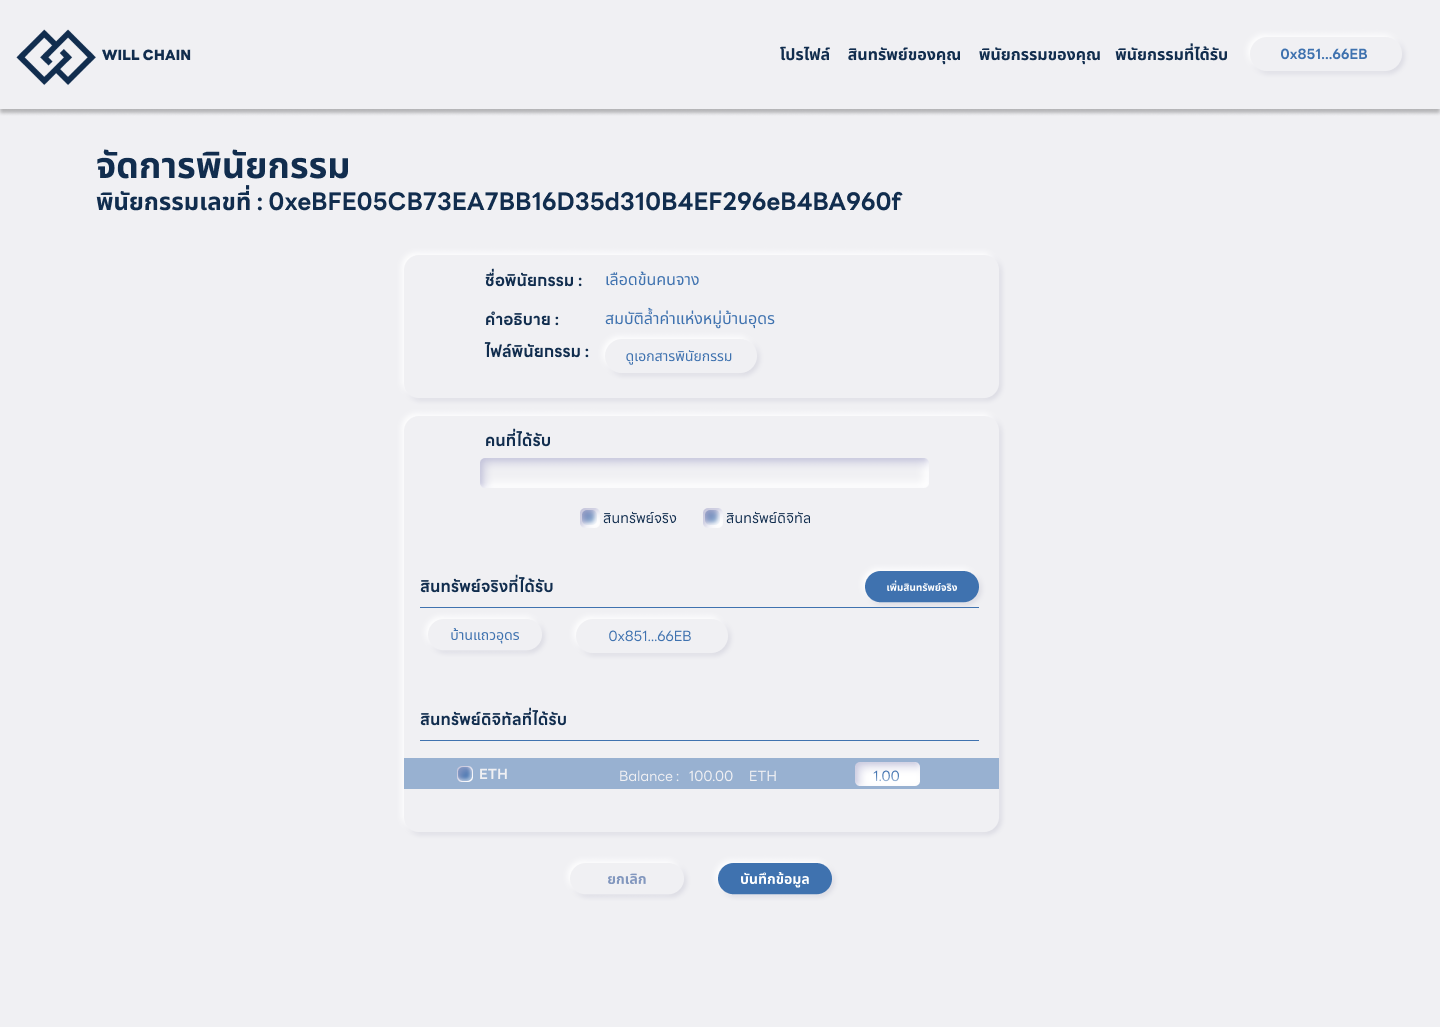
\includegraphics[scale=0.2]{manageWill}
			\caption{หน้าจัดการสินทรัพย์ภายในพินัยกรรมของคุณ}
		\end{figure}
		\FloatBarrier
		\tab  จากรูปเป็นจะเป็นหน้ายกเลิกการทำพินัยกรรม จากการที่กดเมนู "จัดการพินัยกรรม" ในหน้าพินัยกรรมของคุณ โดยที่หน้านีจะแสดงการจัดการพินัยกรรมโดยจะแสดงเลขพินัยกรรม , รายละเอียดพินัยกรรม และพินัยกรรมฉบับจริงในรูปแบบไฟล์ โดยหน้านี้จะทำการใส่เลขกระเป๋า metamask ของผู้รับพินัยกรรมได้ , สามารถเพิ่มเหรียญดิจิทัลได้ , และสามารถเพิ่มสินทรัพย์ที่จะทำการ Tokenize ของสินทรัพย์จริงเป็นในรูปของ NFT และแสดงรายละเอียดทรัพย์สินได้
\subsection{หน้าเพิ่มสินทรัพย์จริง}
		\begin{figure}[!thb]
			\centering
			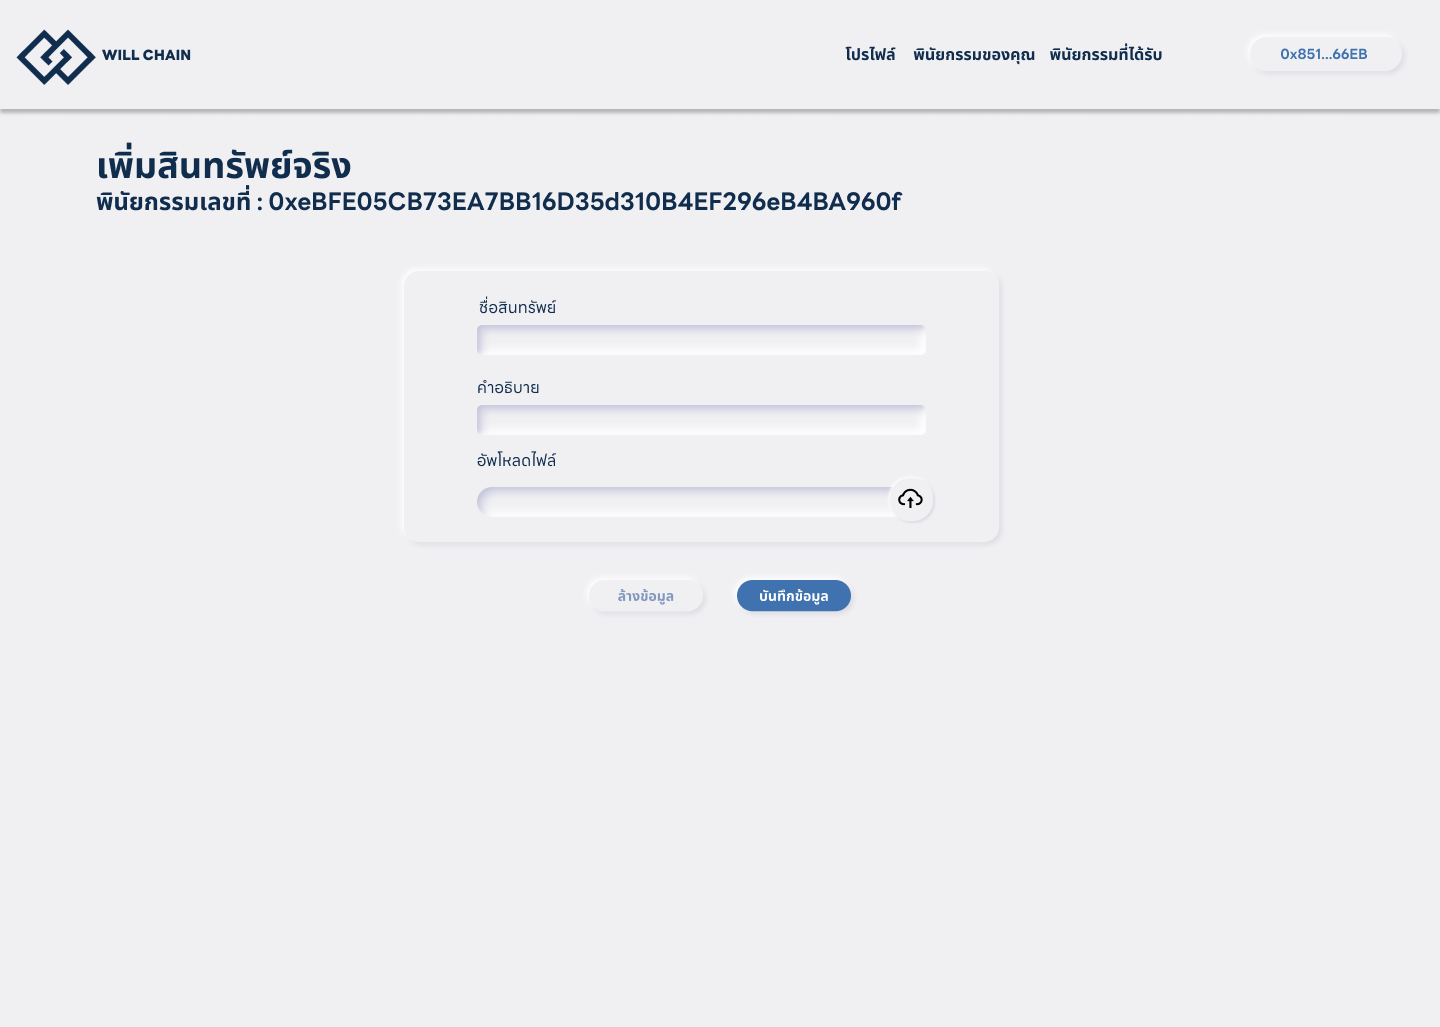
\includegraphics[scale=0.2]{addRealAsset}
			\caption{หน้าเพิ่มสินทรัพย์จริง}
		\end{figure}
		\FloatBarrier
		\tab จากรูปเป็นหน้าเพิ่มสินทรัพย์จริงเข้าสู่พินัยกรรม ที่เมื่อกดที่เมนูสินทรัพย์ในแถบเมนูด้านบน จะเข้าสู่หน้านี้ โดยที่จะแสดงเลขพินัยกรรม และ รายละเอียดของการเพิ่มสินทรัพย์จริงชื่อสินทรัพย์ , คำอธิบาย , และไฟล์สำหรับยืนยันว่าครอบครองพินัยกรรมนั้นจริง ๆ เช่น โฉนดที่ดิน , บ้าน , รถ
\subsection{หน้าพินัยกรรมที่ได้รับ}
		\begin{figure}[!thb]
			\centering
			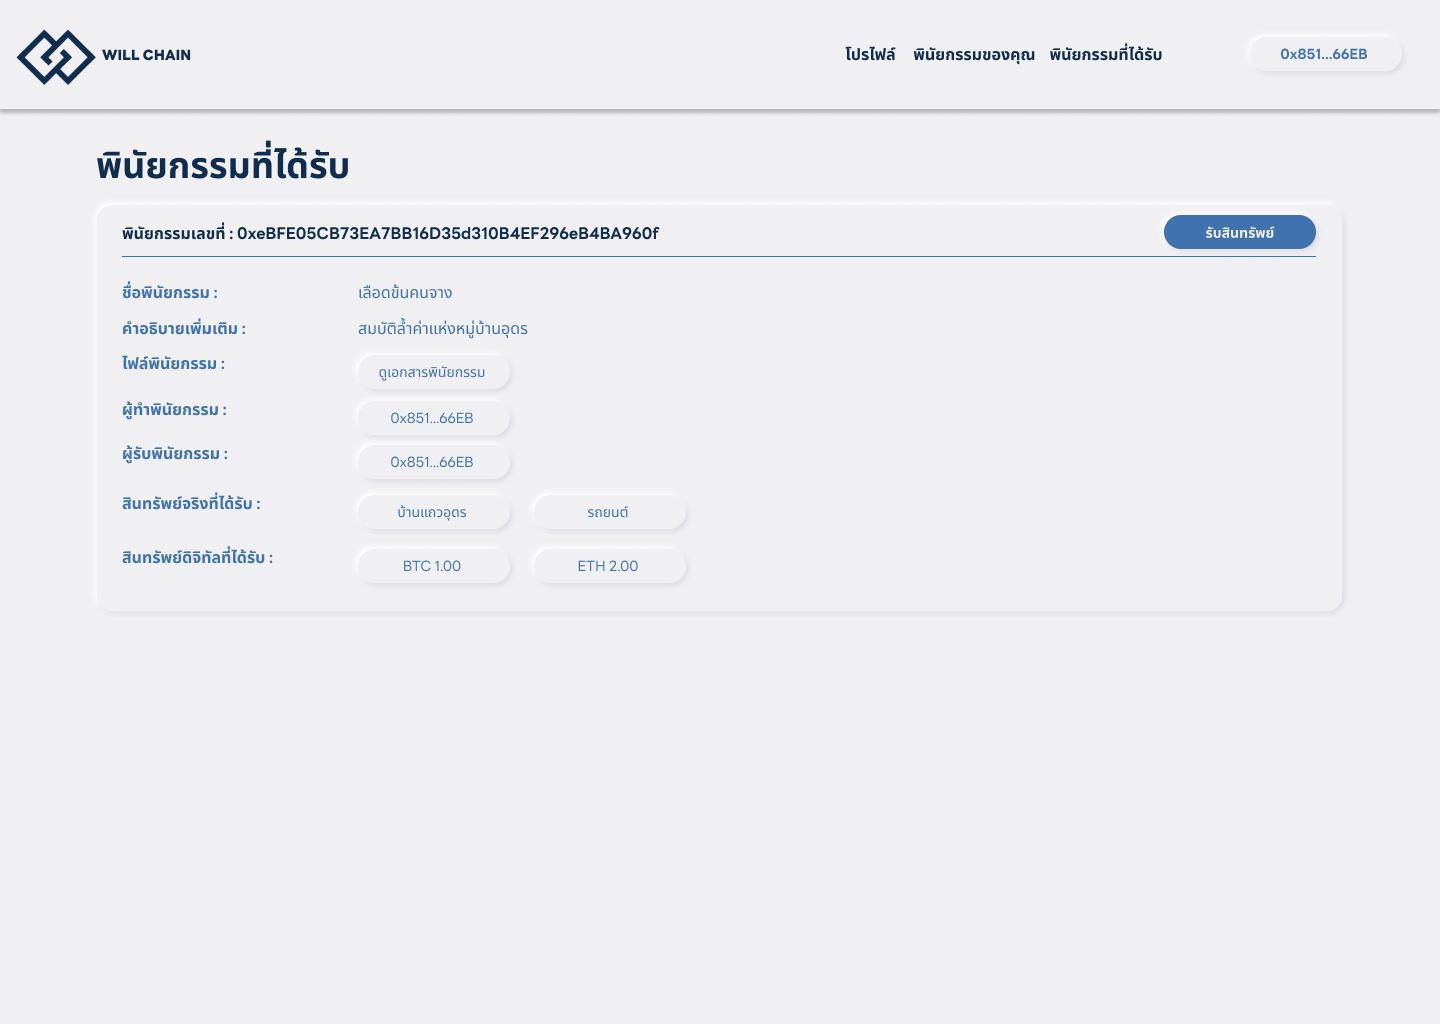
\includegraphics[scale=0.2]{claimWill}
			\caption{พินัยกรรมที่ได้รับ}
		\end{figure}
		\FloatBarrier
		\tab จากรูปเป็นหน้าพินัยกรรมที่ได้รับ ที่หลังจากมีการส่งต่อพินัยกรรมเนื่องมาจากการเสียชีวิต ในหน้านี้จะแสดงพินัยกรรมที่ได้รับ โดยที่สามารถกดปุ่ม “ดูพินัยกรรม” ที่จะสามารถดูพินัยกรรมที่เป็นฉบับจริงได้ และในตารางจะมีแสดงรายละเอียดของคนที่ได้รับ สินทรัพย์ที่ได้รับ และสินทรัพย์ดิจิทัลที่ได้รับ และสามารถกดรับสินทรัพย์ทั้งหมดได้ 
\subsection{หน้ายืนยันรับพินัยกรรม}
		\begin{figure}[!thb]
			\centering
			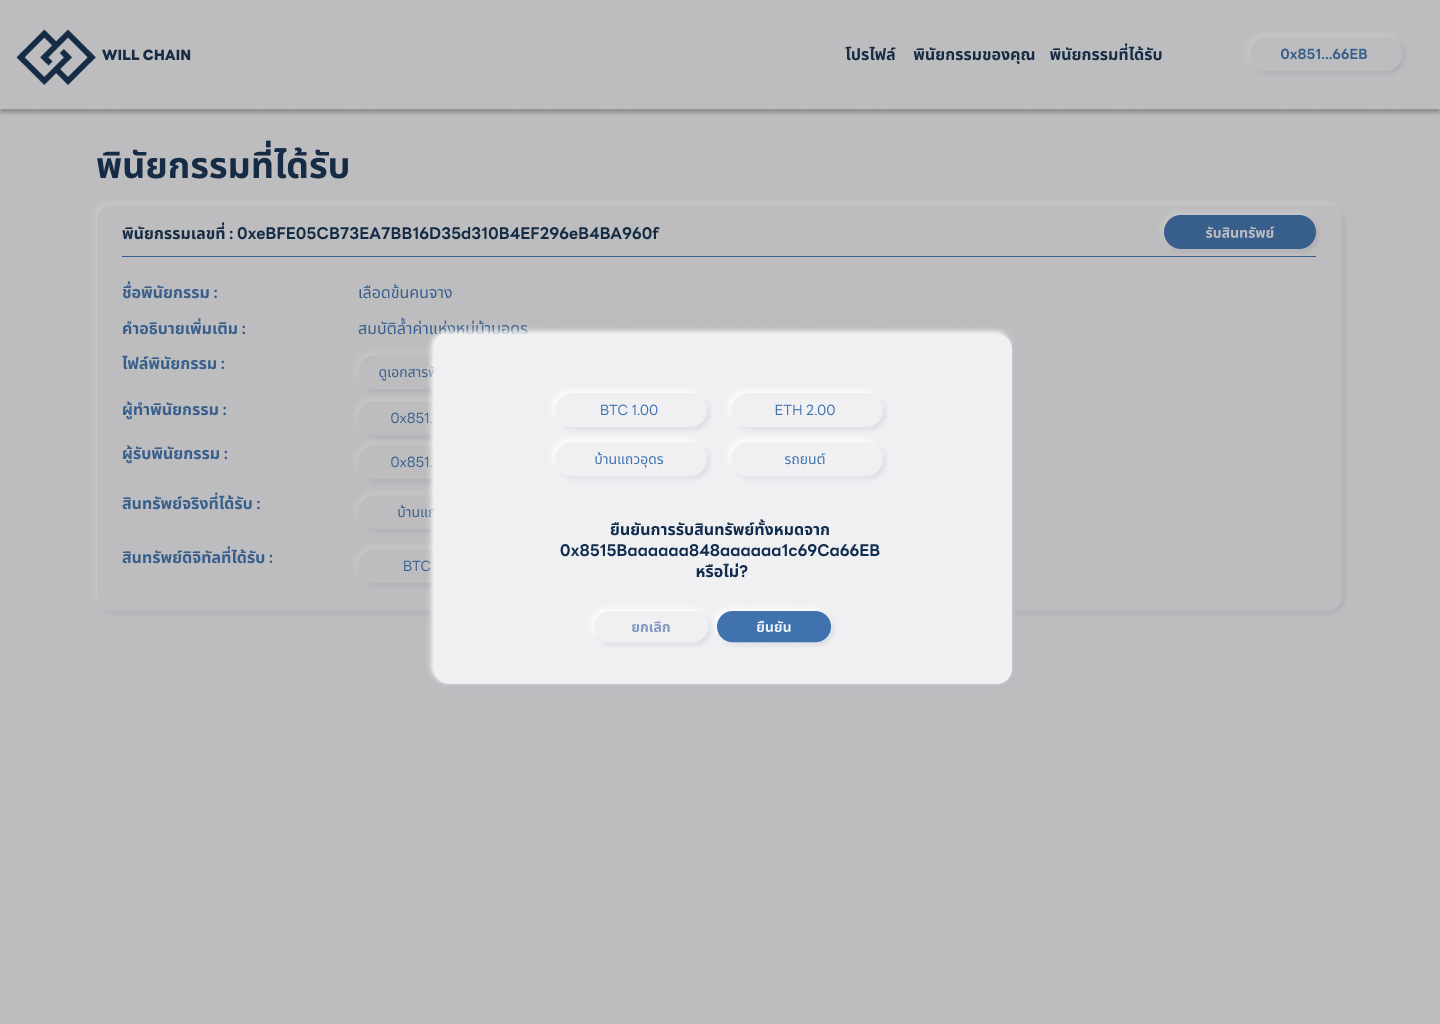
\includegraphics[scale=0.2]{claimWillConfirm}
			\caption{หน้ายืนยันรับพินัยกรรม}
		\end{figure}
		\FloatBarrier
		\tab จากรูปเป็นหน้ายืนยันการรับพินัยกรรมโดยจะทำการเลือกสินทรัพย์ที่ได้รับในแต่ละสินทรัพย์ที่อยู่ในพินัยกรรม
\subsection{หน้ารับพินัยกรรมเสร็จสิ้น}
		\begin{figure}[!thb]
			\centering
			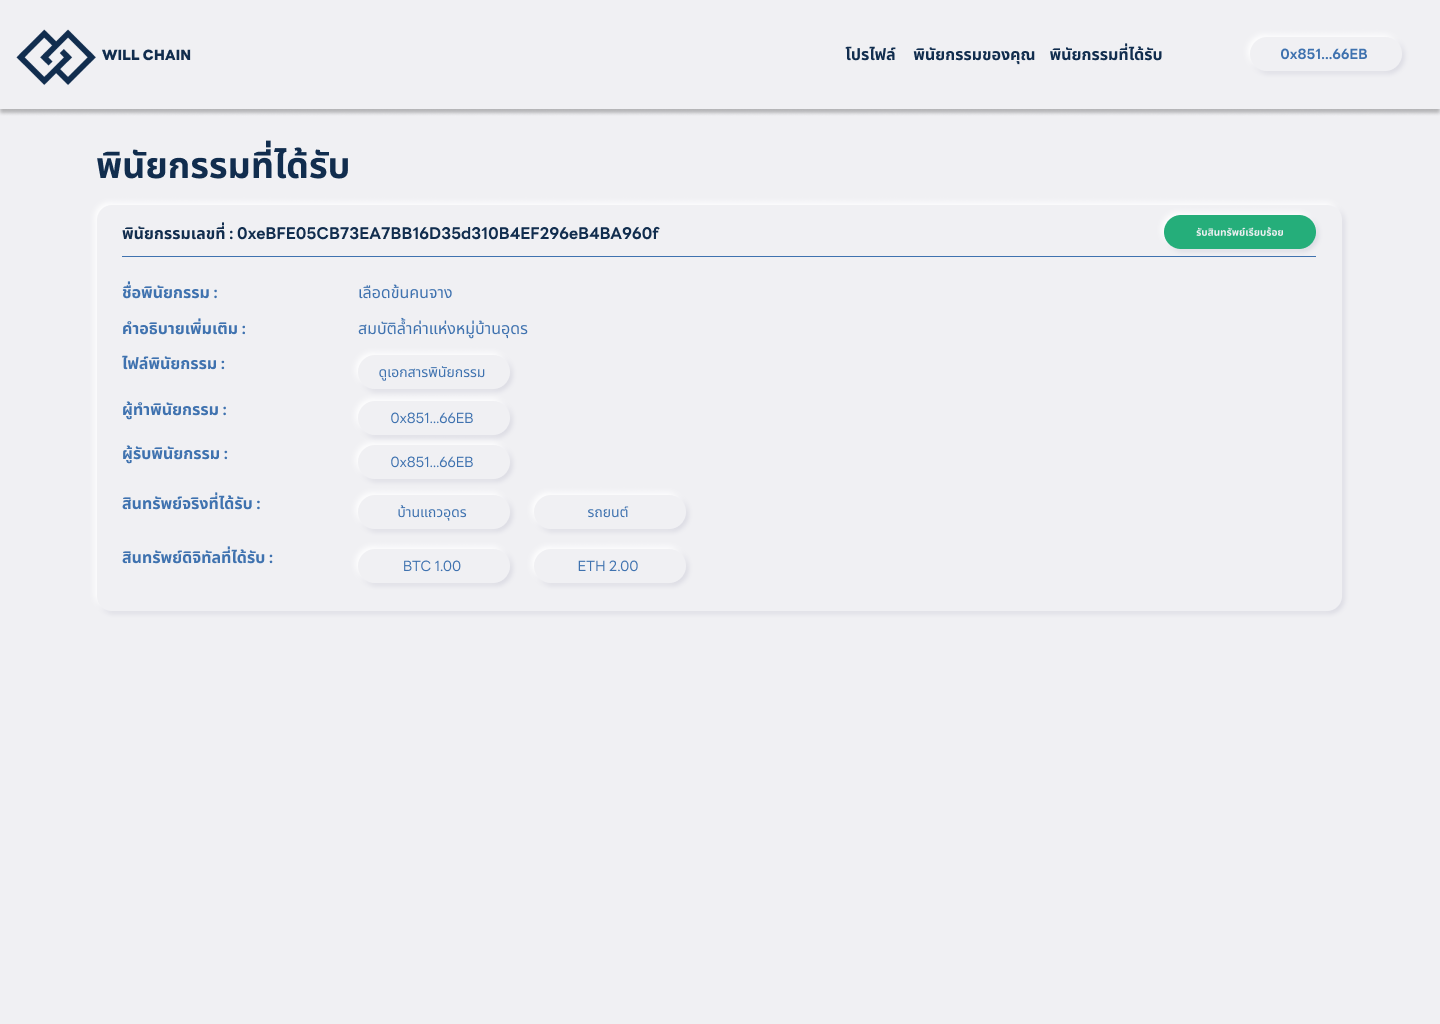
\includegraphics[scale=0.2]{claimWillSuccess}
			\caption{หน้ารับพินัยกรรมเสร็จสิ้น}
		\end{figure}
		\FloatBarrier
		\tab จากรูปเป็นหน้ารับพินัยกรรมเสร็จสิ้น โดยจะเป็นหน้าที่รับสินทรัพย์และรับพินัยกรรมเสร็จสิ้น
\section{ออกแบบการทดสอบ}
\tab ทดสอบด้วยการจำลองการใช้งานผ่าน platform โดยมี function ที่จะทดสอบดั้งนี้
	\begin{enumerate}[label=\thesection.\arabic*,leftmargin=0pt,itemindent=1.25cm]
		\item Function connect MetaMask wallet สําหรับการเชื่อมต่อ wallet ของผู้ใช้งานเข้ากับ MetaMask เพื่อเตรียมพร้อมต่อการทดสอบ function อื่น ๆ
		\item Function เกี่ยวกับการจัดการพินัยกรรมรวมถึงการเพิ่มผู้รับผลประโยชน์และสินทรัพย์ 
		\item Function เกี่ยวกับการจัดการสิยทรัพย์ที่ผู้ใช้ทำการลงทะเบียนไว้ในระบบ
		\item Function การส่งพินัยกรรมและสินทรัพย์ไปให้ผู้รับมรดก
	\end{enumerate}

\chapter{ผลการดําเนินงาน}
\section{Site map}
\begin{enumerate}[label=\thesection.\arabic*,leftmargin=0pt,itemindent=1.25cm]
	\item หน้าหลัก
	\item หน้าโปรไฟล์
	\begin{itemize}[leftmargin=0pt,itemindent=1.25cm]
		\item[-] ลงทะเบียนด้วยรหัสเลขบัตรประชาชน
	\end{itemize}
	\item หน้าพินัยกรรมที่บันทึกของคุณ
	\begin{itemize}[leftmargin=0pt,itemindent=1.25cm]
		\item[-] ทำการ Approve พินัยกรรมของคุณ
		\item[-] ยกเลิกการทำพินัยกรรม
	\end{itemize}
	\item หน้าบันทึกพินัยกรรม 
	\begin{itemize}[leftmargin=0pt,itemindent=1.25cm]
		\item[-] อัพโหลดพินัยกรรม
	\end{itemize}
	\item หน้าจัดการพินัยกรรม
	\begin{itemize}[leftmargin=0pt,itemindent=1.25cm]
		\item[-] เพิ่มสินทรัพย์
		\item[-] เพิ่มผู้รับพินัยกรรม
	\end{itemize}
	\item พินัยกรรมที่ได้
	\begin{itemize}[leftmargin=0pt,itemindent=1.25cm]
		\item[-] รับสินทรัพย์
	\end{itemize}
\end{enumerate}
\section{Token ที่ใช้ใน Will-Chain}
\begin{enumerate}[label=\thesection.\arabic*,leftmargin=0pt,itemindent=1.25cm]
	\item Will Token \\
			\tab \tab  Will Token คือ NFT ที่ทำหน้าที่แทนพินัยกรรมซึ่งทำงานบนระบบ Ethereum โดยใช้มาตรฐาน ERC-721 ซึ่ง Will Token จะเป็นตัวที่ต้องใช้ในการที่เราจะสร้างรับสินทรัพย์ที่มีอยู่ในพินัยกรรมของ Will Contract
	\item ETH \\
			\tab \tab ETH คือ เหรียญดิจิทัลที่ใช้เทคโนโลยีบล็อกเชนทำงานอยู่เบื้องหลัง เพื่อใช้จ่ายสำหรับค่าธรรมเนียม สำหรับทุก Smart Contract ที่ผู้ใช้งานต้องการจะใช้บน Ethereum chain
	\item Any Token Support ERC20\\
			\tab \tab Any Token Support ERC20 คือเหรียญที่ใช้มาตรฐาน ERC-20 ที่ซึ่งใช้เพื่อสำหรับฝากเหรียญดิจิทัลเข้าสู่ระบบของเรา
\item Real Token	\\		
\tab \tab Real Token คือ NFT ที่ทำหน้าที่แทนสินทรัพย์จริงซึ่งทำงานบนระบบ Ethereum โดยใช้มาตรฐาน ERC-721 
	\end{enumerate}
\section{Test Plan}
\begin{enumerate}[label=\thesection.\arabic*,leftmargin=0pt,itemindent=1.25cm]
\item Validation Testing \\
\tab \tab ตรวจสอบว่า Software ตรงตาม Requirement หรือไม่\\
\tab \tab บันทึกข้อผิดพลาดพร้อมกับการแก้ไข
\item Verification Testing \\
\tab \tab ตรวจสอบว่า Software ออกแบบได้ตรงตาม UX/UI ที่ออกแบบไว้หรือไม่\\
\tab \tab ตรวจสอบว่า Software ออกแบบได้ตรงตาม Architecture หรือไม่\\
\tab \tab ตรวจสอบว่า Software ออกแบบได้ตรงตาม UML design หรือไม่\\
\end{enumerate}
\clearpage
\section{Software Testing}
\tab System Testing จะใช้การทำ Unit Testing โดยทำการแยกการทดสอบเป็น function ต่าง ๆ ดังนี้
\subsection {Test Case}
\begin{table}[h]
\begin{tabular}{|l|l|l|}
\hline
Page                   & Test case                                        &  Result \\ \hline
Profile                & ใส่รหัสบัตรประชาชนถูกต้อง                        &        \\ \hline
                       & ใส่รหัสบัตรประชาชนที่ไม่มีในระบบ                 &        \\ \hline
                       & ใส่รหัสบัตรประชาชนไม่ครบ/เกิน                    &        \\ \hline
                       & เลือก menu สินทรัพย์                             &        \\ \hline
                       & เลือก menu พินัยกรรม                             &        \\ \hline
                       & เลือก menu พินัยกรรมที่ได้รับ                    &        \\ \hline
สินทรัพย์ของคุณ        & เลือกเพิ่มสินทรัพย์                              &        \\ \hline
                       & เลือกลบสินทรัพย์                                 &        \\ \hline
                       & เลือกดูข้อมูลสินทรัพย์                           &        \\ \hline
บันทึกสินทรัพย์        & กรอกข้อมูลปรกติแล้วกดบันทึก                      &        \\ \hline
                       & ไม่กรอกชื่อสินทรัพย์                             &        \\ \hline
                       & ไม่เลือกข้อมูลเพิ่มเติม                          &        \\ \hline
                       & ไม่อัพโหลดไฟล์สินทรัพย์                        &        \\ \hline
                       & เพิ่มจำนวนสินทรัพย์                              &        \\ \hline
                       & กรอกข้อมูลสินทรัพย์ไม่ครบทุกหน้า                 &        \\ \hline
รายชื่อคนรับมรดก       & เลือกเพิ่มรายชื่อ                                &        \\ \hline
                       & เลือกลบรายชื่อ                                   &        \\ \hline
พินัยกรรมของคุณ        & เลือกเพิ่มพินัยกรรม                              &        \\ \hline
                       & เลือกลบพินัยกรรม                                 &        \\ \hline
                       & เลือกดูข้อมูลพินัยกรรม                           &        \\ \hline
บันทึกพินัยกรรม        & กรอกข้อมูลปกติแล้วกดบันทึก                      &        \\ \hline
                       & ไม่กรอกชื่อพินัยกรรม                             &        \\ \hline
                       & ไม่อัพโหลดไฟล์พินัยกรรม                        &        \\ \hline
                       & ไม่เลือกผู้ได้รับมรดก                            &        \\ \hline
                       & ไม่เลือกชนิดของสินทรัพย์ที่ได้รับ                &        \\ \hline
                       & เลือกชนิดของสินทรัพย์ไม่ตรงกับสินทรัพย์ที่ได้รับ &        \\ \hline
                       & มอบสินทรัพย์มากว่าที่มีอยู่                      &        \\ \hline
หน้าพินัยกรรมที่ได้รับ & เลือกดูพินัยกรรม                                 &        \\ \hline
                       & กดรับสินทรัพย์ก่อนเวลา                           &        \\ \hline
                       & กดรับสินทรัพย์เมื่อถึงเวลา                       &        \\ \hline
\end{tabular}
\end{table}
\tab หลังจากผ่าน System testing แล้วจะนำไปให้ User ทำการทดสอบว่าตอบสนองความต้องการหรือไม่ โดยจะนำไปให้บุคคลที่มี สินทรัพย์ดิจิทัลที่มีความต้องการที่จะทำพินัยกรรมทดลองใช้ Will Chain ของเรา

\begin{itemize}
	\item[-] ความง่ายในการใช้งาน
	\item[-]  ความน่าเชื่อถือของ Software
	\item[-]  ความเสถียร ของ Software
\end{itemize}
\subsection {Test Smart Contract}
\begin{enumerate}[label=\thesubsection.\arabic*,leftmargin=0pt,itemindent=1.25cm]
\item การทดสอบ Smart Contract ด้วย Hardhat Testing
	\tab การทดสอบด้วย Hardhat Testing ผู้จัดทำได้ออกแบบทดสอบของ Smart Contract ด้วยแบ่งเป็น Flow ในการเรียกใช้งานในแต่ละ Test Case เพื่อให้ครอบคลุมทุกเงื่อนไขในแต่ละฟังก์ชั่น
\begin{figure}[!thb]
			\centering
			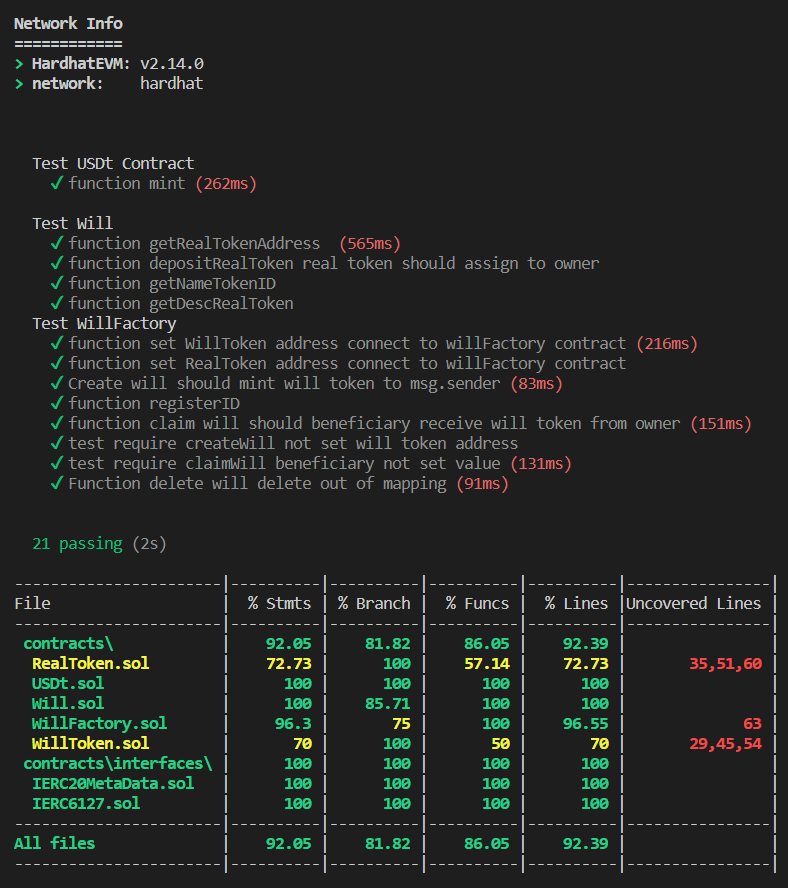
\includegraphics[scale=0.5]{testCoverage}
			\caption{ผล Test Coverage ของ Smart Contract}
		\end{figure}
\FloatBarrier
\tab จากรูป เป็นการออกแบบ Test Case ให้ครอบคลุมทุกฟังก์ชั่นโดยจากภาพจะมีค่า Test Coverage โดย \\ \tab\%Stmts เป็นตัวชี้วัดวัดเปอร์เซ็นต์ของคำสั่งรหัสที่ถูกดำเนินการในระหว่างการทดสอบ ระบุจำนวนบรรทัดของโค้ดที่ถูกเรียกใช้อย่างน้อยหนึ่งครั้ง \\ \tab\%Branch เป็นตัวชี้วัดวัดเปอร์เซ็นต์ของ code ที่ได้รับระหว่างการทดสอบ ตรวจสอบโดยเป็นการตรวจสอบเงื่อนไขของตัว Smart Contract  \\ \tab\%Funcs เป็นตัวชี้วัดเปอร์เซ็นต์ของฟังก์ชันที่ถูกเรียกใช้ในระหว่างการทดสอบ จะตรวจสอบว่าแต่ละฟังก์ชันได้รับการดำเนินการอย่างน้อยหนึ่งครั้งหรือไม่  \\\tab\%Lines เป็นตัวชี้วัดเปอร์เซ็นต์ของความครอบคลุมของบรรทัดของ code โดยจะวัดเปอร์เซ็นต์ของบรรทัดโค้ดที่ดำเนินการระหว่างการทดสอบ
\end{enumerate}

\section{การ Deploy Smart Contract ไปที่ Ethereum Chain}
	\tab การ Deploy Smart Contract ไปที่ Ethereum Chain โดยเป็น Test network เพื่อความรวดเร็วในการ Deploy Smart Contract และไม่มีค่าธรรมเนียมในการทำธุรกรรมต่าง ๆ ในการทำงานของระบบ โดยใช้ Hardhat ในการทำการ Deploy Smart Contract โดยมีขั้นตอนดังนี้
	\\\tab 1. ต้องทำการ Deploy Contract WillFactory ซึ่งเป็น Contract ที่ใช้สำหรับการจัดการพินัยกรรมทั้งหมดและจัดการการสืบทอดพินัยกรรมของพินัยกรรมทั้งหมด
	\\\tab 2. ทำการ Deploy Contract Will Token เพื่อที่จะทำการ Tokenize ของพินัยกรรมและเป็น NFT มาตรฐาน ERC-721 โดย Will Token ไม่สามารถถ่ายโอนให้คนอื่นได้ด้วยตัวเอง แต่จะสามารถถ่ายโอนได้ ผ่าน Contract WillFactory เท่านั้น
	\\\tab 3. ทำการ Deploy Contract Real Token เพื่อที่จะทำการ Tokenize ตัวสินทรัพย์จริงและสินทรัพย์นี้จะทำการสร้าง NFT มาตรฐาน ERC-721 โดย Real Token จะไม่สามารถถ่ายโอนให้คนอื่นได้ด้วยตัวเอง แต่จะสามารถถ่ายโอนได้ ผ่าน Contract Will เท่านั้น
	\\\tab 4. ทำการ Deploy Contract USDt เพื่อที่จะทำการจำลองสินทรัพย์ดิจิทัลประเภทเหรียญในระบบ โดยจะเป็นมาตรฐาน ERC-20 ใช้สำรองทดสอบการฝากด้วย Token ที่นอกเหนือจาก ETH
	\\\tab 5. ทำการ Deploy Contract Will เป็นการ Contract ที่สร้างขึ้นมาจาก Will Factory โดย Will Contract จะทำหน้าที่ค่อยเก็บพินัยกรรมของเจ้าของพินัยกรรมและจัดการพินัยกรรมสินทรัพย์ในระบบทั้งหมด
\\\tab 	ผลลัพท์ของการ Deploy Smart Contract จะได้ Contract Address ดังนี้
\\\tab willFactory deployed to: 0x54BeBcd2469AAE5E4417f4c6d01d2C8Eb31331cC
\\\tab willToken deployed to: 0x9f2c24a6aB735C9ECFbF2e8d1A36CD8F54D2248F 
\\\tab USDt deployed to: 0xe25ddff621198069bA7fe5A18f3D94C1f6F60496 
\\\tab RealToken deployed to: 0x7d7Ce3e5Be7Be44FC38F9A73046D2d79735d552f
\\\tab โดย Will Contract จะถูกสร้างด้วย WillFactory และ Smart Contract ทั้งหมดจะถูก verify เพื่อความถูกต้องและความปลอดภัยด้วย Hardhat verify โดย Smart Contract ที่ verify แล้วจะแสดงผลได้ที่หน้า Etherscan ที่เป็น block explorer และ สามารถใช้ฟังก์ชั่นใน Contract  ได้ผ่าน หัวข้อ Contract 
\begin{figure}[!thb]
			\centering
			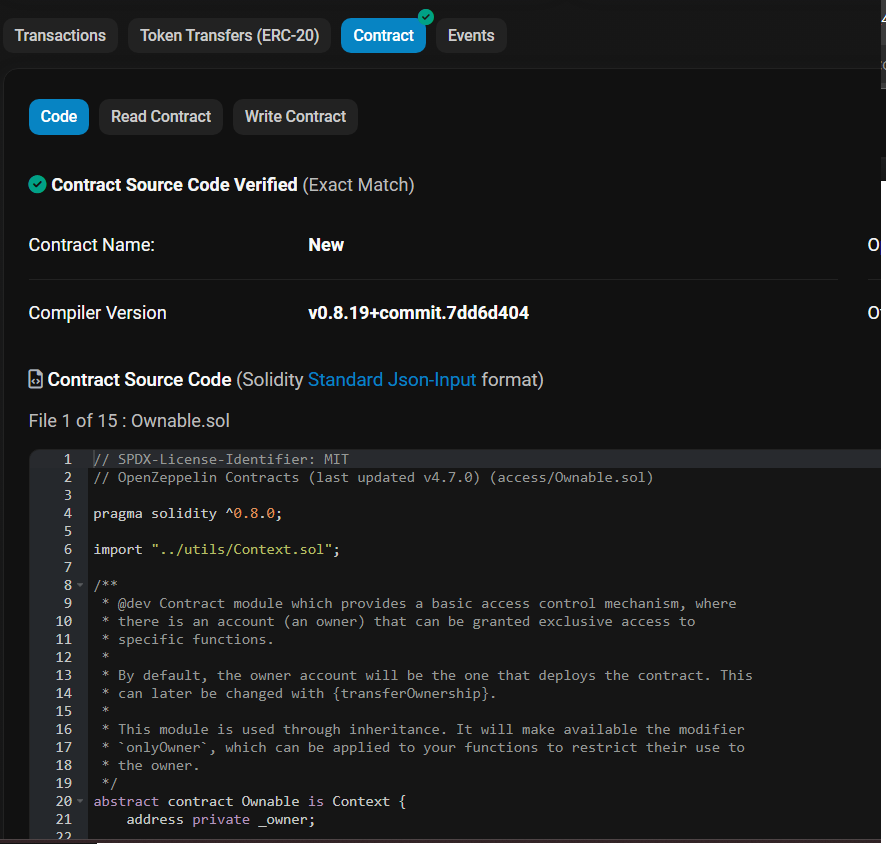
\includegraphics[scale=0.5]{etherscan}
			\caption{แสดงผล code หลัง verified contract}
		\end{figure}
\begin{figure}[!thb]
			\centering
			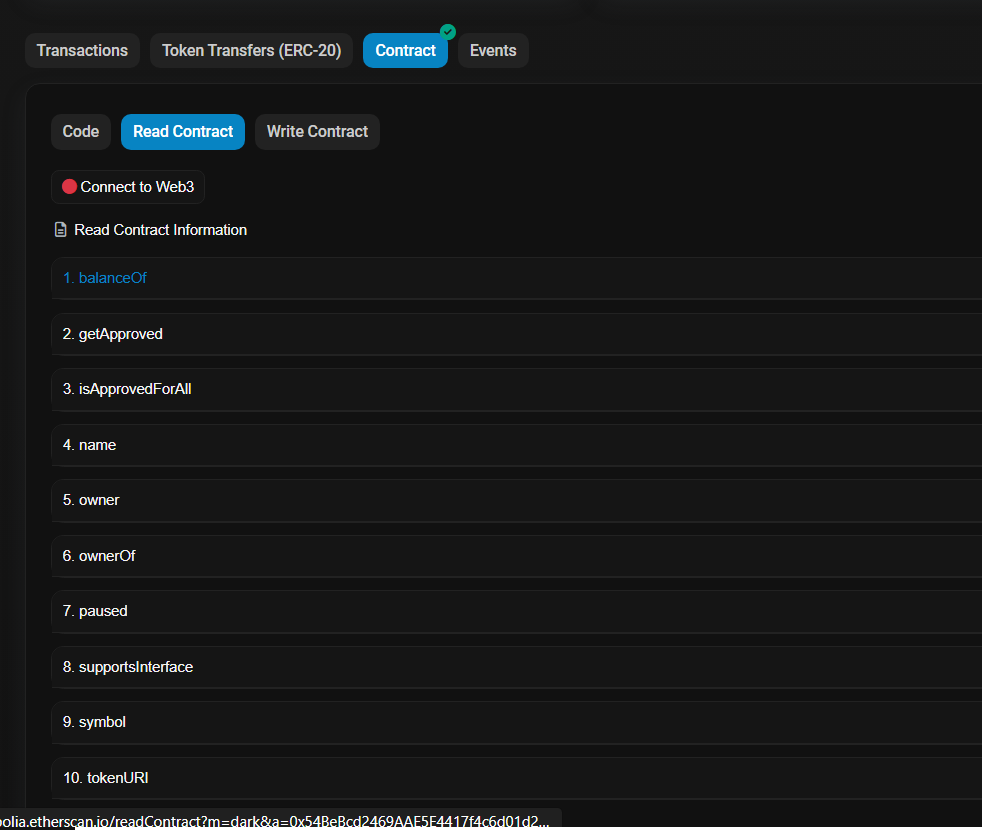
\includegraphics[scale=0.5]{etherscanRead}
			\caption{แสดงฟังก์ชั่นสำหรับที่แสดงผล หลัง verified contract}
		\end{figure}
\begin{figure}[!thb]
			\centering
			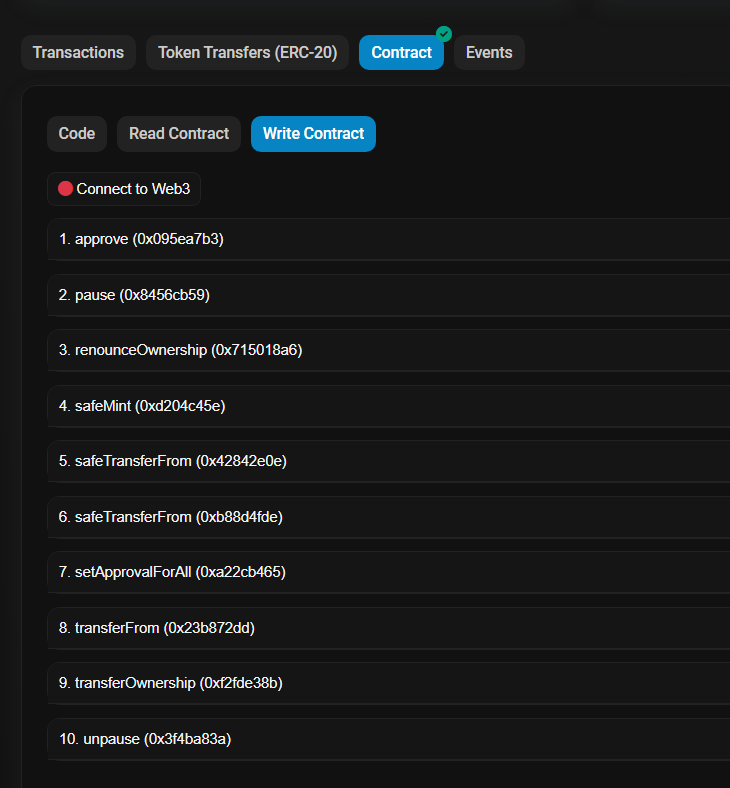
\includegraphics[scale=0.5]{etherscanWrite}
			\caption{แสดงฟังก์ชั่นที่มีการเขียนลงระบบ ethereum chain หลัง verified contract}
		\end{figure}
\chapter{สรุปผล}
\section{ สรุปปัญหาที่พบและวิธีการแก้ไข}
\subsection{Design System}
\tab ปัญหาที่พบ 1 : Design ที่ทำมาในช่วงแรกไม่สามารถ implement ได้เนื่องจากขาดความรู้ความเข้าใจในตัวของ Tech Stack ของระบบทำให้มีการปรับแก้ไขในส่วนของ Design System ใหม่ และ ส่งผลให้ทุกส่วนในด้านการทำงานของระบบต้องมีการ design ใหม่\\
\tab การแก้ไข : คือทำการ Design ระบบใหม่ระหว่างช่วงที่ทำการ Develop ไปพร้อม ๆ กัน\\

\subsection{Process Management}
\tab ปัญหาที่พบ 1 : จากเหตุผลของ Design System ส่งผลให้กระทบการวางแผนและประเมินเวลาในแต่ละวีค \\
\tab การแก้ไข : เพิ่ม workload ในแต่ละวีคและเพิ่ม goal ในแต่ละวีคว่าอะไรต้องเสร็จก่อนเป็นลำดับ\\

\subsection{Blockchain}
\tab ปัญหาที่พบ 1 : ไม่มี Token ของสินทรัพย์ดิจิทัลให้ทดสอบกับตัว Contract \\
\tab การแก้ไข : เลือกใช้วิธีการสร้าง Contract USDt ซึ่งเป็นเหรียญที่ใช้ interface ตัวเดียวกันกับของที่มีอยู่ใน blockchain
\subsection{Smart Contract}
\tab ปัญหาที่พบ 1 : ไม่สามารถทำการส่งพินัยกรรมให้ผู้รับพินัยกรรมที่มีในระบบมากกว่าสองคนได้ใน พินัยกรรมเดียว\\
\tab การแก้ไข : ทำการสร้างพินัยกรรมที่เป็น Will Contract สำหรับจัดการ 1 พินัยกรรมต่อ 1 คน และถ้ามีหลายคน ก็ใช้พินัยกรรมเดิมในสร้าง Will Contract ขึ้นมาใหม่\\
\tab ปัญหาที่พบ 2 : มีปัญหาเรื่องของการกำหนดเงื่อนไขว่าใครสามารถทำอะไรบ้างในแต่ละคอนแทค\\
\tab การแก้ไข : ทำการใช้ interface AccesControl เป็นตัวช่วยในการจัดการ Role และ เพิ่ม role ของ smart contract\\
\tab ปัญหาที่พบ 3 : มีปัญหาเรื่องการการ estimate gas ไม่ได้ ตอนที่ทำการ Transfer จาก Will Contract ไปที่กระเป๋าของผู้รับพินัยกรรม\\
\tab การแก้ไข : ทำการ approve token ของเจ้าของพินัยกรรมนั้นก่อนทำการส่งไปที่ Contract\\
\tab ปัญหาที่พบ 4 : ไม่สามารถใช้งาน API เช็คการเสียชีวิตจากกรมการปกครองได้
\tab การแก้ไข : ทำการ Assume ส่วน API เช็คการเสียชีวิตแทนด้วย AccessControl เป็น Role Controller เพื่อทำการ Control การเสียชีวิตของผู้ทำพินัยกรรม
\subsection{Frontend}
\tab ปัญหาที่พบ 1 : ทำการเชื่อมต่อ metamask ได้ยาก\\
\tab การแก้ไข : ทำการใช้ตัว thirdparty ในการเชื่อมต่อกับ metamask wallet\\
\section{สถานะการดำเนินงาน}
\section{สรุปผลการดำเนินงาน}
\subsection{Will}
\tab สามารถแสดงผลของรายละเอียดพินัยกรรม โดยเปิดให้ผู้ใช้งานมาใช้ได้ด้วยการกรอกเลขบัตรประชาชนไปที่หน้าของ register id card หลังจากนั้นเจ้าของพินัยกรรมจะสามารถใช้งานระบบได้และมีการแสดง componet ที่ให้ผู้ใช้สร้างพินัยกรรม และ สามารถเพิ่มสินทรัพย์ดิจิทัล ที่ใช้มาตรฐาน ERC-20 รวมถึงการทำ tokenize ของสินทรัพย์จริงได้ โดยพินัยกรรมจะทำงานก็ต่อเมื่อมีการเสียเกิดขึ้นโดยจะมี role ที่ทำการควบคุมคือ controller ซึ่งจะสามารถทำให้พินัยกรรมส่งไปหาผู้รับพินัยกรรมผ่านกระเป๋า metamask wallet\\
\subsection{Will Token}
\tab สามารถแสดงผลของการทำ tokenize ของตัวพินัยกรรม โดยตัว Will Token จะทำหน้าที่เป็นพินัยกรรมโดยถ้าผู้รับพินัยกรรมไม่ถือ เหรียญ Will Token ที่ผูกกับพินัยกรรมนั้น ก็จะไม่สามารถ ใช้งานพินัยกรรมในระบบหรือถอนสินทรัพย์ออกจากระบบได้\\
\subsection{Claim Assets}
\tab สามารถรับสินทรัพย์จากการที่ role controller ที่ควบคุมของการดำเนินการของการส่งพินัยกรรมก่อนจึงจะสามารถรับสินทรัพย์ในระบบได้ โดยสามารถรับสินทรัพย์ดิจิทัลที่ใช้ มาตรฐาน ERC-20 และ สามารถรับสินทรัพย์จริงในรูปแบบของ NFT ที่ทำ tokenize จากสินทรัพย์จริงได้มาสู่ผู้รับพินัยกรรม\\

\subsection{แนวทางในการพัฒนาในอนาคต}
\tab แนวทางในการพัฒนาโครงงานต่อในอนาคตจะเป็นเรื่องของการติดต่อฝ่ายกรมการปกครองเพื่อทำการใช้งาน API เช็คการเสียชีวิตและนำมา implement ในระบบ และ จะทำเรื่องการ soulbound token ในการทำการยืนยันตัวตนและทำการเก็บข้อมูลของผู้ใช้ไว้ที่นั้นเพื่อให้ระบุตัวตนได้ง่ายขึ้นรวมถึงการเพิ่มระบบ multisig wallet สำหรับกรณีที่ผู้ใช้ไม่อยากฝากสินทรัพย์หรืออะไรไว้ในระบบของเรา ซึ่งจะสะดวกในการใช้งานมากกว่าโดย mulsig wallet จะเป็นการเลือกผู้รับพินัยกรรมที่สามารถ approve เอาเลขกระเป๋าของกระเป๋าหลักที่ทำการทำพินัยกรรมไว้ และสามารถเลือกจำนวนคนที่สามารถ approve ของกระเป๋าได้\\


 
%%%%%%%%%%%%%%%%%%%%%%%%%%%%%%%%%%%%%%%%%%%%%%%%%%%%%%%%%%%%%%%
%%%%%%%%%%%%%%%%%%%% Bibliography %%%%%%%%%%%%%%%%%%%%%%%%%%%%%
%%%%%%%%%%%%%%%%%%%%%%%%%%%%%%%%%%%%%%%%%%%%%%%%%%%%%%%%%%%%%%%

%%%% Comment this in your report to show only references you have
%%%% cited. Otherwise, all the references below will be shown.
%\nocite{*}
%% Use the kmutt.bst for bibtex bibliography style 
%% You must have cpe.bib and string.bib in your current directory.
%% You may go to file .bbl to manually edit the bib items.

\makeatletter
\g@addto@macro{\UrlBreaks}{\UrlOrds}
\makeatother

\bibliographystyle{kmutt}
\bibliography{string,cpe}

%%%%%%%%%%%%%%%%%%%%%%%%%%%%%%%%%%%%%%%%%%%%%%%%%%%%%%%%%%%%%%%
%%%%%%%%%%%%%%%%%%%%%%%% Appendix %%%%%%%%%%%%%%%%%%%%%%%%%%%%%
%%%%%%%%%%%%%%%%%%%%%%%%%%%%%%%%%%%%%%%%%%%%%%%%%%%%%%%%%%%%%%%



%%%%%%%%%%%%%%%%%%%%%%%%%%%%%%%%%%%%%%%%%%%%%%%%%%%%%%%%%%
%%%%%%%%%%%%%%% The 2nd appendix %%%%%%%%%%%%%%%%%%%%%%%%%%
%%%%%%%%%%%%%%%%%%%%%%%%%%%%%%%%%%%%%%%%%%%%%%%%%%%%%%%%%%






\end{document}
